\documentclass[12pt]{ucthesis}

\usepackage{etex}
\usepackage[morefloats=125]{morefloats}
\usepackage[hyphens]{url}
%\usepackage{subfig}
\usepackage{subcaption}
\usepackage{graphicx}
\usepackage{transparent}
\usepackage{tabularx}
\usepackage{amssymb}
\usepackage{amsmath}
\usepackage{empheq}
\usepackage[letterpaper]{geometry}
\usepackage[overload]{textcase}
\usepackage{color}
\usepackage[nonumberlist,toc]{glossaries}
\usepackage{wrapfig}
\usepackage{longtable}
\usepackage{morefloats}
\usepackage{float}
\usepackage{listings}
\usepackage{makecell}
\usepackage{appendix}
\usepackage[]{algorithm2e}
\usepackage{titlesec}
\usepackage[breaklinks=true,hidelinks,pdfusetitle]{hyperref}
\usepackage{cleveref}
\usepackage{ifthen}
\usepackage{tikz}
\usepackage{import}
\usepackage{pgfplots}
%\usepackage{showframe}

\usetikzlibrary{plotmarks}
\providecommand{\e}[1]{\ensuremath{\times 10^{#1}}}
\newcommand{\volume}{{\ooalign{\hfil$V$\hfil\cr\kern0.08em--\hfil\cr}}}
\newcommand{\T}{\textbf{{\tiny \textsf{T}}}}
\newcommand{\bunderline}[2][4]{\underline{#2\mkern-#1mu}\mkern#1mu }
\makeindex
\makeglossaries
\graphicspath{{./figures/}}
% Shrink the size of headers
\titleformat{\chapter}[display]
        {\normalfont\normalsize\centering}
        {\ifthenelse{\equal{\thechapter}{A}}{APPENDICES\\[4.3ex]}{}\chaptertitlename\ \thechapter}
        {0pt}{\normalsize\uppercase}
\titlespacing*{\chapter}{0pt}{-20pt}{4.3ex plus .2ex}


\titleformat*{\section}{\normalsize\bfseries}
\titleformat*{\subsection}{\small\bfseries}
\titleformat*{\subsubsection}{\small\bfseries}
\titleformat*{\paragraph}{\small\bfseries}
\titleformat*{\subparagraph}{\small\bfseries}

\bibliographystyle{abbrv}

\setlength{\parindent}{0.25in} \setlength{\parskip}{6pt}
\geometry{verbose,nohead,tmargin=1in,bmargin=1in,lmargin=1.5in,rmargin=1in}
\setcounter{tocdepth}{4}

% Different font in captions (single-spaced, bold) ------------
\newcommand{\captionfonts}{\small\bf\ssp}

\newcommand{\mycaption}[2]{\caption[#1 --- #2]{#1 --- #2}}

\makeatletter  % Allow the use of @ in command names
\long\def\@makecaption#1#2{%
  \vskip\abovecaptionskip
  \sbox\@tempboxa{{\captionfonts #1: #2}}%
  \ifdim \wd\@tempboxa >\hsize
    {\captionfonts #1: #2\par}
  \else
    \hbox to\hsize{\hfil\box\@tempboxa\hfil}%
  \fi
  \vskip\belowcaptionskip}
\makeatother   % Cancel the effect of \makeatletter
% ---------------------------------------

% Define Appendix refs
\crefname{app}{appendix}{appendices}
\Crefname{app}{Appendix}{Appendices}

\begin{document}

% Declarations for Front Matter
\title{Rotordynamic Analysis of Theoretical Models and Experimental Systems }
\author{Cameron Naugle}
\degreemonth{April} \degreeyear{2018} \degree{Master of Science}
\defensemonth{January} \defenseyear{2018}
\numberofmembers{3}
\chair{Xi (Julia) Wu, Ph.D. \linebreak Professor of Mechanical Engineering}
\othermemberA{Mohammad Noori, Ph.D. \linebreak Professor of Mechanical Engineering}
\othermemberB{Peter Schuster, Ph.D. \linebreak Professor of Mechanical Engineering}
\field{Mechanical Engineering} \campus{San Luis Obispo}
\copyrightyears{seven}

\maketitle

\begin{frontmatter}

% Custom made for Cal Poly (by Mark Barry, modified by Andrew Tsui).
\copyrightpage

% Custom made for Cal Poly (by Andrew Tsui).
\committeemembershippage

\begin{abstract}
This thesis is intended to provide fundamental information for the construction and analysis of rotordynamic theoretical models, and their comparison the experimental systems. Finite Element Method (FEM) is used to construct models using Timoshenko beam elements with viscous and hysteretic internal damping. Eigenvalues and eigenvectors of state space equations are used to perform stability analysis, produce critical speed maps, and visualize mode shapes. Frequency domain analysis of theoretical models is used to provide Bode diagrams and in experimental data full spectrum cascade plots. Experimental and theoretical model analyses are used to optimize the control algorithm for an Active Magnetic Bearing on an overhung rotor.
\end{abstract}

\begin{acknowledgements}
\noindent
Thanks to:
\begin{itemize}
    \item Bently Nevada for their support through the Donald E. Bently Center for Engineering Innovation at Cal Poly. The equipment provided by Bently Nevada made this work possible.
    \item My Advisor, Xi Wu, for always thinking big, and for supporting all my work.
    \item My family and friends for their support and love.
\end{itemize}

\end{acknowledgements}

\tableofcontents

\listoftables

\listoffigures

% Add CHAPTER into table of contents.
\addtocontents{toc}{%
   \noindent CHAPTER
}

\end{frontmatter}

\pagestyle{plain}

\renewcommand{\baselinestretch}{1.66}

\chapter{Introduction}
\section{Background} 
The study of rotating machines is a relatively new branch of mechanics, the study of which began in the late 1800's with the industrial revolution catalyzing a need to mitigate dangerous vibrations of machines, such as the steam turbine. Increasing demands on power generation were leading to increased size and speed of such turbines, which in turn increased the need to understand how and why they produced vibrations. Engineers, for an extended period of time, thought it was impossible to operate continuously at a speed above the first critical speed (a speed at which the rotation excites a natural frequency in the system). One of the first papers published on the matter by Rankine in 1869 even posited this as fact--that rotors could not be stable above this first critical speed. Jeffcott produced one of the first meaningful solutions to the rotrodynamic problem in 1919 with his model that is now known as the Jeffcott rotor. This rotor is a simple model with a single disk located equidistant from two bearing supports. In his paper he articulates his realization that after the first critical speed, a rotor in this configuration is self centering (begins to rotate about its center of mass). This realization motivated engineers to design systems that could withstand forces involved with passing through the first critical speed and operate in the supercritical range. In general, operating in this supercritical range allowed machines to operate more efficiently and effectively.\par 
Today our understanding of rotordynamics has led to the operation of  machines that spin at speeds of over a hundred thousand revolutions per minute--many times the first critical speed. The incorporation of computers in to the study of rotordynamics has accelerated innovation, allowing new rotors to push even these boundaries. Additionally, increasing use of adaptive control devices such as the Active Magnetic Bearing (AMB) allows for more control over the vibration of rotating machines. Control of rotor systems permits adaptability after design and adjustment to varying operating conditions. \par
Rotors developed today are increasingly complex. The trend in new applications is to incorporate rotordynamic analysis in the design process, rather than fixing already built systems. As rotordynamic analysis becomes increasingly integral in the design process, the Finite Element Method (FEM) is proving to be a vital design tool. FEM is widely used in many other fields, such as structures and impact analysis. With FEM, design parameters can be optimized in terms of geometry and material properties to minimize vibration. Though commonly used FEM packages can be altered for use in rotordynamics, it is often the case the elements included are not designed with consideration of gyroscopic moments. Gyroscopic moments fundamentally change the dynamics of a rotating sytem, especially at high speeds. Thus, their inclusion in FEM is vitally important to produce accurate results.\par 
An array of FEM packages exist to specifically design rotordynamic models that meet the complexity demanded by modern applications (including gyrospcopic moments) such as: DyRoBeS, DYNROT, and XLRotor. These packages provide valuable design information on complex linear and non-linear FEM models.\par
\section{Literature Review}\label{LiteratureReview}
Nelson \& McVaugh \cite{nelson1976dynamics} introduced an early Finite Element for use in rotordynamics that included gyroscopic moments in 1976. This model used a Bernoulli-Euler beam to define the internal bending stiffness of the beam element. The Bernoulli-Euler beam does not include shear effects, limiting its use to relatively slender beams. Nelson made an improvement to this model in 1977, with Zorzi \cite{zorzi1977finite} with the inclusion of rotating internal damping in the constitutive relationship in the form of viscous and hysteretic damping mechanism. Nelson (1980, \cite{nelson1980finite}) then extended his 1976 model to include shear deformation of the beam element, with the addition of shear this element is known as the Timoshenko beam element. But, he did not include internal viscous or hysteretic damping in the model. Ozguven, in 1984\cite{ozguven1984whirl}, extended Zorzi's 1980 Timoshenko model to include shear deformation effects.  An excellent derivation of the Timoshenko beam element is provided by Luo (2008)\cite{luo2008efficient}. His derivation results in the static homogeneous Euler-Lagrangian differential equations pertaining to bending, axial, and torsional motion. Additionaly, Luo provides a derivation of the shape interpolation functions that reduce shear locking in the Timoshenko beam element. All beam models described thus far assume a homogeneous beam for each element. Derivations of beam models exist that do not assume a homogeneous beam, such as the paper on conical beam elements by Greenhill, Bickford, and Nelson in 1985\cite{greenhill1985conical}, and the paper on consistent beams from Genta in 1985\cite{genta1985consistent}. This non-homogeneous extension is not realized in the model presented in this work. Genta's textbook on rotordynamics, published in 2007\cite{genta2007dynamics} involves a detailed derivation of the finite element equations using the Timoshenko beam and shear-lock reducing shape interpolation functions.\par 
Important anecdotal notes on understanding of the rotating damping effect are presented in Kandil's 2004\cite{kandil2005rotor} thesis ``On Rotor Internal Damping Instability.'' Kandil presents a strong physical description of the internal damping effect and the many sources it has. Further interpretations for the effect of internal damping were presented by Genta in his paper ``On a Persistent Misunderstanding of the Role of Hysteretic Damping in Rotordynamics,'' where the common misunderstanding of sub-critical instability due to hysteretic damping is rectified.\par 
The use of Bernoulli-Euler beam elements in the application of a vibration reducing Active Magnetic Bearing (AMB) is presented in the paper from Das, et al. (2008\cite{das2008vibration}). Das also provides the derivation of a simple control algorithm for the AMB using a linearized magnetic force equation.\par
Frequency domain analysis of rotordynamic models specifically is discussed in Genta's 2007 textbook ``Dynamics of rotating systems,''\cite{genta2007dynamics}. Additional overview of frequency domain analysis for vibrations in general is provided by Craig in the 2006 textbook ``Fundamentals of structural dynamics,''\cite{craig2006fundamentals}. Time domain analysis of vibration signals is also discussed in this text. Agnes Muszynska lends understanding for the concept of complex spectrum, and interpretations specific for rotordynamics in her 2005 ``Rotordynamics'' textbook, \cite{muszynska2005rotordynamics}, and her paper published with Goldman in 1999 on the matter \cite{goldman1999application}.
\section{Scope of Work}
This work will be comprised of: 
\begin{itemize}
	\item methods for analyzing time domain vibration signals to produce information on frequency content, amplitude, and phase lag, as well as discussion of where these time domain signals come from and the requirements for accurate system characterization.
	\item construction of a finite element model specifically formulated for use in rotating beams.
	\item frequency domain analysis of rotordynamic models for the assessment of critical speeds, mode shapes, stability, and damping characteristics.
	\item Synthesis of signal analysis of experimental data with frequency domain analysis of finite element models to optimize the performance of an active magnetic bearing supporting an overhung disk rotor system.
\end{itemize}
This work will not deeply explore time domain signal processing, frequency domain analysis, or the finite element method, but is intended to provide an overview of these topics and how they pertain to rotating machinery. This work was developed with the intention to aid in the continued exploration of rotordynamics at Cal Poly.\par
\chapter{Vibration Signal Analysis}
\section{Data Collection and Processing}
The most important measurement to be made in order to perform significant rotordynamic analysis is the Vibration Signal, $ V $ or $ W $. Other beneficial measurements include Spin Speed, $ \Omega $, of the rotating shaft (especially important if during a start-up or run-down), and a Reference Signal, $ R $, that indicates a rotational position of the shaft. Orthogonal vibration signals (meaning two independent directions), $ V\ \&\ W $, measuring the position of the shaft centerline can help in characterizing anisotropic systems. Sampling Rates, $ f_s $ of the signals mentioned thus far must be high enough to measure the vibration of interest, typically this is at least several times the highest expected rotation speed of the shaft. It is important to note that these signals can come from an experiment or a theoretical model.\par
There are four variables deduced from the above signals that form the basis for the majority of rotordynamic figures and analysis. These are Amplitude of Vibration, $ A[m,mils] $, Amplitude Spectrum, $ \tilde{A}(\omega)[m,mils] $, Phase of Vibration, $ \beta[\deg,Rad] $, and Spin Speed, $ \Omega[Hz,Rad/s,RPM] $. Amplitude Spectrum is actually a two dimensional variable where the dependent variable, $ \omega[Hz,Rad/s,RPM] $, represents the Frequency of Vibration (or Whirl Speed if its in units of rotation). Figures to be presented in this work are varying combinations of these four variables. The Bode diagram plots $ A $ against $ \Omega $ alongside $ \beta $  against $ \Omega $. A Spectrum figure plots $ \tilde{A}(\omega) $. An extension of this is the Cascade which adds the third dimension of $ \Omega $. Orbit plots represent one cycle of the time domain signals $ V\ \&\ W $. Lastly, 3D Orbits are formed by plotting the orbit($ V,W $) against $ \Omega $. Explanations of the importance and methods in producing these plots are to follow. \par
A difficulty in rotordynamic analysis arises in the continuous change of $ \Omega $ causing a continuous change in the dependent variables $ A,\ \tilde{A}(\omega),\ \&\ \beta $, a visualization of these changes is visualized in Figure \ref{fig:PosOverTime}. This poses difficulty because the techniques used to produce $ A,\ \tilde{A}(\omega),\ \&\ \beta $ from $ V,\ W\&\ R $ rely on a span of subsequent rotations. A solution to this dilemma utilized in this work is the discretization of signals $ X,\ Y,\ R\ \&\ \Omega $ into windows in time. The window, whose width will be represented by the variable $ nspw[samples] $. There is a trade off between accuracy and resolution of variables as $ nspw $ is changed. This trade off will be elaborated on in \S\ref{Resolution}.\par 
\begin{figure}
	\centering
	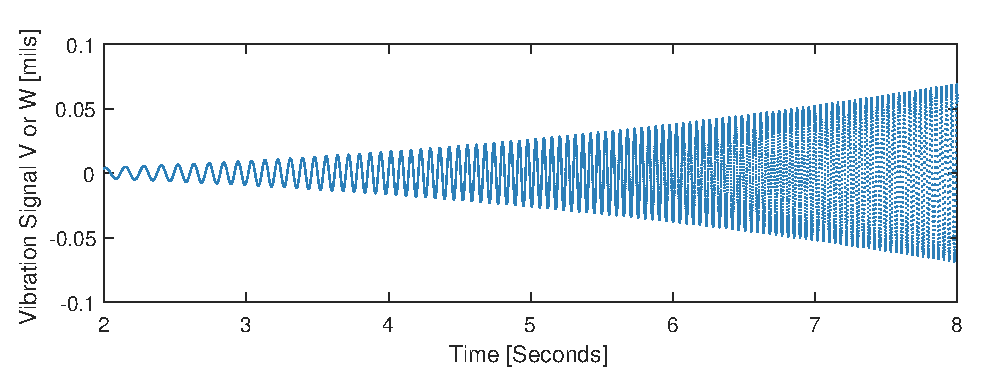
\includegraphics[width=\linewidth]{./figures/Pos_Over_Time.eps}
	\caption{Position of the rotor shaft over a certain timespan.}
	\label{fig:PosOverTime}
\end{figure}
The windowing approach is visually depicted using $ \Omega $ in figure \ref{fig:SpeedWindow} as it changes over time. When the width of the window is small enough, such as in Figure \ref{fig:FreqSpanWindow}, the change in the independent variable becomes vanishingly small. Other continuous variables such as $ A,\ \tilde{A}(\omega),\ \&\ \beta $ are expected to behave similarily, in that their value may be approximated by a single number, or in the case of $ \tilde{A}(\omega) $ as a single spectrum, inside the window despite the change in that variable throughout the entire length of time.
\begin{figure}
	\begin{subfigure}{.5\textwidth}
	\centering
	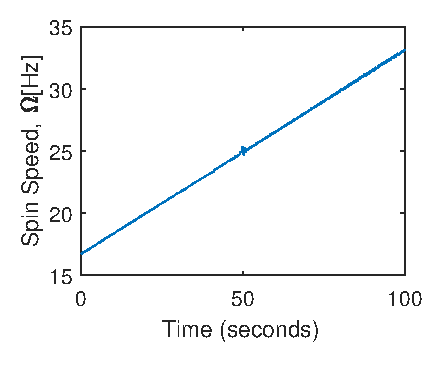
\includegraphics[]{./figures/FrequencySpan.eps}
	\caption{Rotor speed change over time during a ramp up.}
	\label{fig:FreqSpanOverTime}
\end{subfigure}
\begin{subfigure}{.5\textwidth}
	\centering
	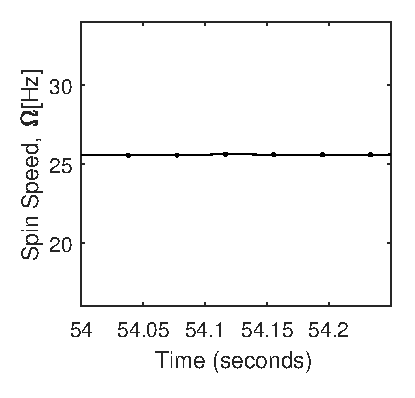
\includegraphics{./figures/FrequencyWindow.eps}
	\caption{Rotor speed change over time during a ramp up.}
	\label{fig:FreqSpanWindow}
\end{subfigure}
\caption{Rotor Spin Speed Windowing effect.}
\label{fig:SpeedWindow}
\end{figure}
Inside of a window of vibration, as the one shown in Figure \ref{fig:WindowedData} the Speed, Amplitude and Phase all approach constant the smaller $ nspw $ gets.\par
\begin{figure}
	\centering
	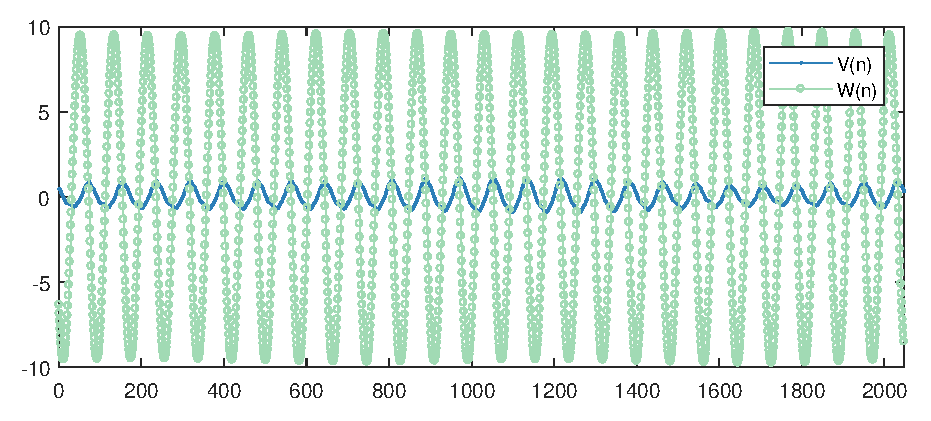
\includegraphics{./figures/SSTime.eps}
	\caption{A window in time of the transient vibration signals for a window, $ nspw $, of $ 2048[samples] $.}
	\label{fig:WindowedData}
\end{figure}
The variables $ V(t) $, $ W(t) $\& $ R(t) $ will now take the form $ V(n) $, $ W(n) $\& $ R(n) $ inside the window (fig. \ref{fig:WindowedData}), where $ n $ is sample number. Spin Speed is simply taken as an average in the window, $ \Omega(N)=avg(\Omega(0:nspw)) $, where $ N $ is the current window index. Therefore, no further explanation is given for its determination. Amplitude, Phase, Amplitude Spectrum, and Spin Speed must be calculated in each window, for a series of windows that cover the entire length of signals. Then a vector of each variable will exist where the length is equal to the number of windows, $ NW $, and is given by
\begin{equation*}
NW = \frac{length(signals)}{nspw}
\end{equation*}\par 
The calculation of each of the variables inside the window, at some $ N $, is given in the following sections. A useful visual representation of the windowed signals $ V(n)\ \& W(n) $ are presented in Figure \ref{fig:WindowedData} to aid in understanding the sections to follow.
\subsection{Amplitude}
Amplitude calculation is fairly straightforward within the window. One approach to calculate the peak to peak amplitude is to take the average over the whole window, $ A_v(N) = max(V(0:nspw))-min(V(0:nspw)) $. Another is to use a peak-finding algorithm to determine the height of each peak and average them all over the sample length. General computer code packages, such as MATLAB,  will contain a peak finding algorithm, the details of which are out of the scope of this work.
\subsection{Spectrum}
The frequency spectrum of the signal is calculated inside the window using a Fourier Transform. In MATLAB the Fast Fourier Transform (fft) has been preprogrammed allowing easy working between time and frequency domains.
\begin{equation}\label{eq:FFTReal}
\tilde{A_V} = \frac{\text{fft}(V)}{nspw},\ \&\ \tilde{A_W} = \frac{\text{fft}(W)}{nspw}
\end{equation}\par 
A useful way to represent the data is using complex variable to compact the two orthogonal displacements $ V\ \&\ W $ as
\begin{equation}\label{eq:ComplexDisplacement}
Z = V + iW
\end{equation}
now the spectrum of this complex value represents both equation planes of vibration in one equation:
\begin{equation}\label{eq:FFTComplex}
\tilde{A}_\pm = \frac{\text{fft}(Z)}{nspw}
\end{equation}\par
Thus far, the frequency spectrum in the real coordinates and in the complex is in terms of samples on the dependent axis. The frequency vector to which the fft() corresponds must be calculated. This is the whirl speed, $ \omega $. It is known that the slope of $ \omega $ is $ d\omega=f_s/nspw $. It is also known that the frequency vector is the same length as the time domain signal 
\begin{equation*}
f(n)=d\omega(0:nspw-1)
\end{equation*}
and to center the spectrum at a frequency of 0
\begin{equation*}
\begin{array}{c}
Q=ceiling((nspw+1)/2)\\
\omega_Q=d\omega(Q-1)\\
\omega=f-fQ
\end{array}
\end{equation*}
where $ \omega $, here in $ Hz $, is the dependent variable that pairs with the real or complex Amplitude spectrum. The Amplitude spectrum in real coordinates(fig.\eqref{eq:FFTReal}) is symmetric for positive and negative $ \omega $, so typically when the spectrum of a single variable is presented in a spectrum plot or in a cascade it is only the positive frequency side presented. On the other hand, the complex representation of the amplitude spectrum(\eqref{eq:FFTComplex}) is not symmetric on the positive and negative sides of $ /omega $. This decomposition can be better understood by realizing the form of the Fourier transform as the summation of circles in the complex plane, $ \tilde{A_\pm}(\omega)e^{i\omega t} $. When $ \omega $ is positive this represents a positive rotation, and when negative represents a negative rotation. For a given whirl speed, $ \omega_i $, this results in sum of a positively rotating circle of amplitude, $ \tilde{A}(\omega_i) $ and a negatively rotating circle of amplitude $ \tilde{A}(-\omega_i) $. The ellipse formed by this summation is the orbit of the shaft centerline at this specific speed. With the understanding of contributions of $ \tilde{A}(\omega) $ and $ \tilde{A}(-\omega) $, we can realize that the resulting ellipse will rotate in the positive direction if $ \tilde{A}(\omega)> \tilde{A}(-\omega) $ and in the negative direction otherwise.
\subsection{Phase}
\subsubsection{Time Domain Approach}
A rather direct way of calculating the phase angle comes from an inspection of the time domain signal. If some once per turn reference is available, then using either a zero-crossing, peak-finding, or threshold algorithm can be employed to reference a specific angle of the shaft rotation. If the vibration signal is mostly synchronous, that is vibrating at the same frequency as the rotation of the shaft, then a peak-finding or zero-crossing algorithm can be used to determine the number of samples from the shaft reference angle to the peak of the vibration.\par 
\begin{equation}\label{eq:PhaseAngleTimeDomain}
\beta_k = 2\pi\frac{\#ref_k-\#peak_k}{\#ref_k-\#ref_{k-1}}
\end{equation}
where $ \beta_k $ is the phase lag of the signal of interest from the reference signal at the $ k $th reference cycle, $ \#ref_k $ is the sample number of the reference trigger, and $ \#peak_i $ is the sample number of the peak of the signal of interest. One large advantage to this brute force method is that is can run continuously and provide current phase information on just the last rotation of the shaft. In the application to the window of vibration data, fig. \ref{fig:WindowedData}, the measurements of each cycle would be averaged across the window as $ \beta(\omega)=avg(\beta_k) $ for however many indexes $ k $ were found in the window. \par 
\subsubsection{Frequency Domain Approach}
Alternatively, the phase angle can be determined using the frequency domain signals.\par 
If the speed of the rotor is known and the time domain signals $ v\ \&\ w $ are known to be synchronous, or filtered to synchronous, then the spectrums of the signals of interest can be used to calculate the phase delay. For any frequency, $ \omega $ the angle is calculated using the equation
\begin{equation*}
\beta(\omega)=angle(\tilde{A}(\omega))-angle(\tilde{K}(\omega))
\end{equation*}
where $ \tilde{K} = \frac{\text{fft}(K)}{nspw} $ is the frequency domain representation of the reference signal. Either $ \tilde{A}_V $ or $ \tilde{A}_W $ is used to find the phase delay of the $ V $ or $ W $ time domain vibration in reference to the once per turn reference of $ K $. It is also possible to find the delay of any time domain signals in reference to any other time domain signal at a specific frequency using the above equation. Though the common practice is to compute the $ \beta $ angle of both signals and subtract one from another. In synchronous vibration, $ \omega=\Omega $.\par
\section{Rotordynamic Figures}\label{ExperimentalPlots}
In the previous section Amplitude, Phase, and frequency spectrum were calculated for the interior of a window of index $ N $. Each of the data then need to be indexed as all of the windows are processed until the entire signal has been exhausted. The total number of windows can be realized in the equation $ NW=\frac{length(X)}{nspw} $ where $ X $ is a placeholder for any time domain signal. After all windows have been exhausted, vectors for $ A,\ \tilde{A}(\omega),\ \beta\ \&\ \Omega $ will all be of length $ NW $.\par 
For the visualization of the plots, experimental data from a overhung rotor system with one disk will used to present the figures.\par
\subsection{Bode}
The Bode diagram for the example overhung rotor system is given in Figure \ref{fig:ExpExampleBode}. First, by looking at the amplitude portion of the plot it si evident that the $ V $ signal undergoes a natural frequency before the $ W $ signal because the peak for $ A_V $ occurs before $ A_W $. This idea is also supported through the inspection of the phase lag portion of the plot, as two seperate transitions are evident. Having two seperate peaks is an indication of high anisotropy of stiffness in the system. By observing the phase lag of each the vertical and the horizontal, it is evident that the orbit direction is opposite the spin speed between speeds ~ 1280-1350[RPM]. This is due to the phase angles switching polarity with one another. If normally horizontal lags vertical, as is suggested by the sub-synchronous and super-synchronous range, then during the critical speed the orbit is reversed since vertical begins to lag horizontal.\par
Bode diagrams are extremely useful in diagnosing unbalance in the system through inspection of the phase lag portion. If the shaft was perfectly straight before any deformation due to rotating unbalance, then the phase lag just before the first natural frequency is the angle of the unbalance vector. This is due to the fact that before the first natural frequency, the unbalance vector is aligned with the vibration radially out from the center of rotation. Furthermore, natural frequencies can be detected through the use of the phase lag information. Phase lag typically shifts $ 180\deg $ through a natural frequency, and is at $ 90\deg $ during one.
\begin{figure}
	\centering
	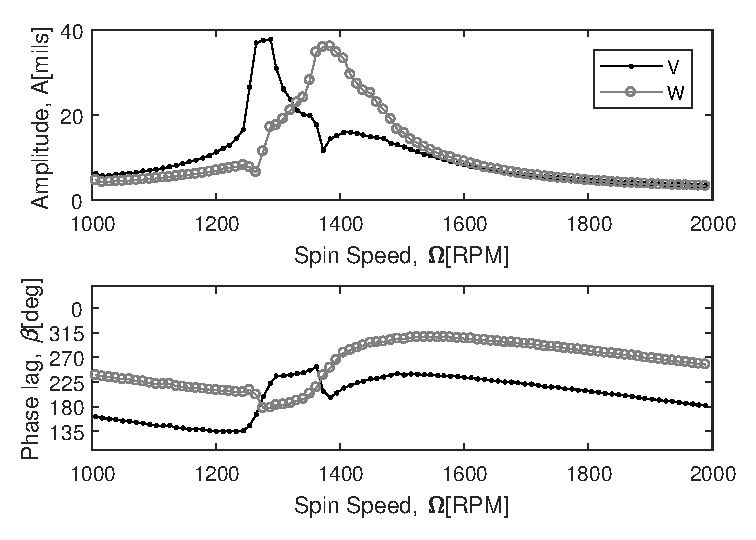
\includegraphics[]{./figures/ExpExampleBode.eps}
	\caption{Bode diagram of the experimental example overhung system. Signals are filtered to synchronous speed.}
	\label{fig:ExpExampleBode}
\end{figure}
\subsection{Full Spectrum and Full Spectrum Cascade}
A single Spectrum at a specific speed is shown as Figure \ref{fig:ExpExampleSpectrum}. This is the Complex representation of the spectrum refered to as the ``Full Spectrum'' of the time domain signal because it contains both positive and negative frequencies. This figure tells us that the orbit at this speed is in the negative whirl direction since the negative amplitude, $ \tilde{A}_\pm(-\omega)=10.27 $ at its peak is greater than $ \tilde{A}_\pm(\omega)=8.80 $. Also, there is minimal amplitude in the spectrum other than this single frequency of $ 31.25[Hz] $ indicating the vibration is highly synchronous.
\begin{figure}
	\centering
	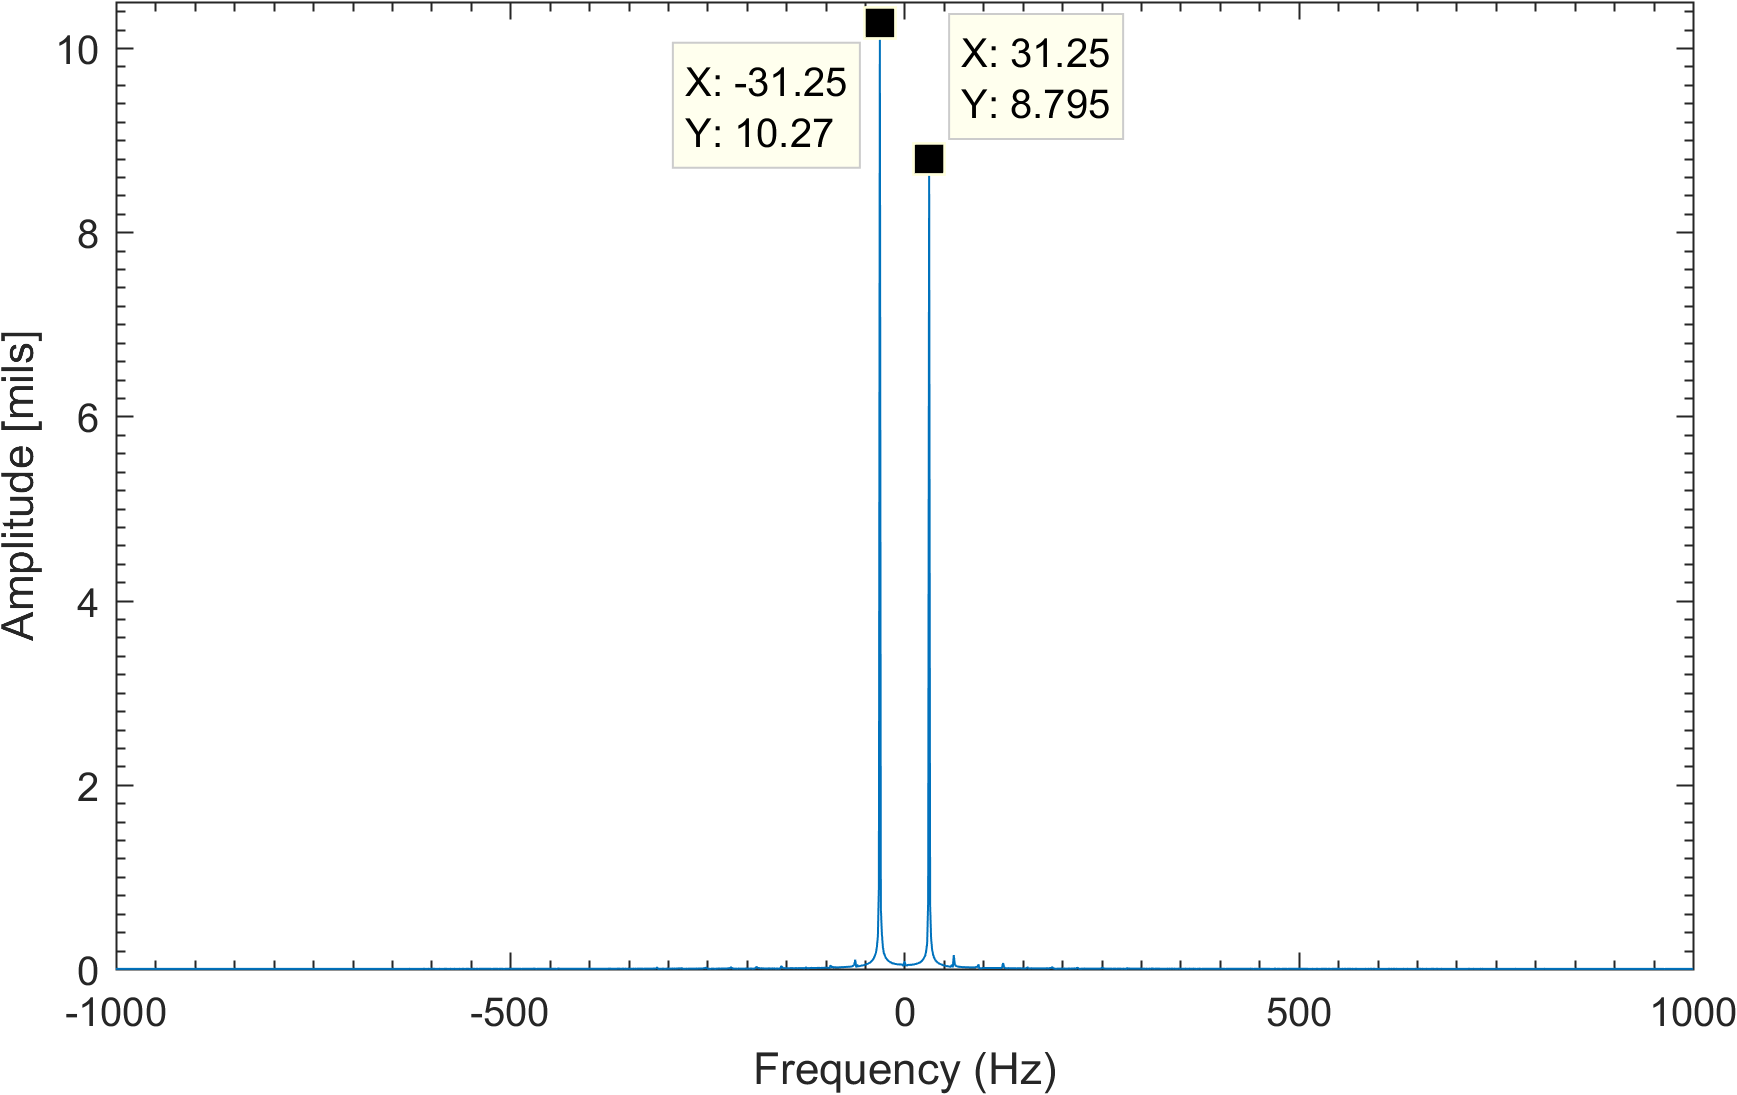
\includegraphics[width=\linewidth]{./figures/Images/Figure_8.png}
	\caption{Example Full Spectrum.}
	\label{fig:ExpExampleSpectrum}
\end{figure}
 A Cascade plot is demonstrated with the experimental system described in \S\ref{ExperimentalPlots}, as Figure \ref{fig:ExpExampleCascade}. Using this figure it is easy to detect the portion of the start-up in which the orbit is whirling opposite the spin speed. A sharp dip in positive amplitude, $ \tilde{A}_\pm(\omega) $, correlated with a sharp rise in negative amplitude, $ \tilde{A}_\pm(-\omega) $, leads to this phenomena.\par 
The Cascade plot is particularly useful in characterizing non-synchronous vibration. Slightly evident in the example cascade of figure \ref{fig:ExpExampleCascade} is the super-synchronous vibration at twice the spin speed, this is often called the 2X vibration and likewise and other non-synchronous whirl can be referenced as nX. The cascade plot is an indispensable tool for the analysis of fluid film bearing as they are characterized by sub-synchronous whirl that is difficult to identify in a Bode Diagram.\par 
\begin{figure}
	\centering
	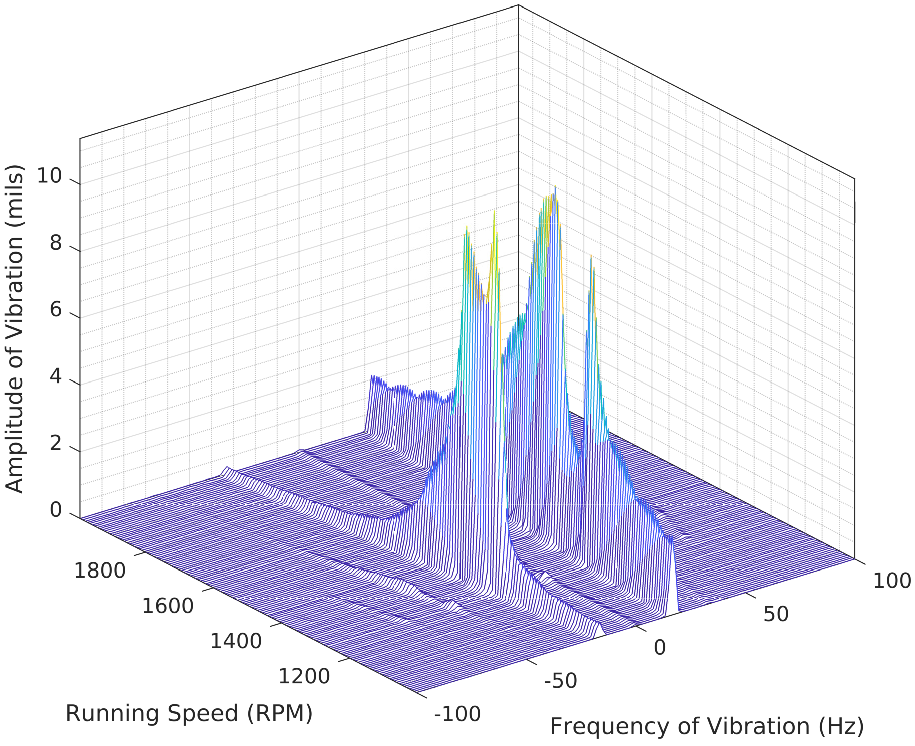
\includegraphics[width=\linewidth]{./figures/ExpExampleCascade.pdf}
	\caption{Cascade of the experimental system described in \S\ref{ExperimentalPlots}.}
	\label{fig:ExpExampleCascade}
\end{figure}
\subsection{Orbit}
Now in the time domain, the actual orbit or trace of the centerline of the shaft is observed. In this work, the orbit is visualized in two ways; as a path in 2D space at a specific spin speed, or as a 3D orbit with a cascade of orbits as spin speed is increased. The 3D Orbit allows for the visualization of complex phenomena in a simple intuitive way. Figure \ref{fig:ExpExample3DOrbit} 3D Orbit is given for the experimental example described in \S\ref{ExperimentalPlots}. Appearing, once again is evidence of the negative whirl in the critical speed range. In the 3D orbit a necking of the shape can be seen between the speeds of 1200-1400[RPM] indicating the orbit has reversed its direction. Looking at independent orbits at specific speeds should explicitly demonstrate the orbit necking and turning negative. In Figure \ref{fig:ExpExampleOrbits} at speed $ 1194[RPM] $ the orbit is clearly whirling in the positive direction, as speed increases the orbit collapses into a line between speeds $ 1203\ \&\ 1206[RPM] $ and begins whirling in the negative direction until the process is reversed by speed $ 1289[RPM] $. Therefore, it can be confirmed that the orbit is whirling backward between the speeds ~1205-~1280[RPM].\par
\begin{figure}
	\centering
	\includegraphics[width=\linewidth]{./figures/ExpExample3DOrbit.eps}
	\caption{3DOrbit of the experimental system described in \S\ref{ExperimentalPlots}. Lighter colors indicate larger vibration.}
	\label{fig:ExpExample3DOrbit}
\end{figure}
\begin{figure}
\begin{subfigure}{.28\linewidth}
	\def\width{\linewidth}
	\pgfplotsset{every picture/.style={scale=1},every axis/.style={title style={yshift=-.8em}}}%, every axis/.style={hide axis}}%
	\centering
	\import{figures/}{ExpExampleOrbit1194.tex}
	\label{fig:ExpExampleOrbit1194}
\end{subfigure}
\begin{subfigure}{.28\linewidth}
	\def\width{\linewidth}
	\pgfplotsset{every picture/.style={scale=1},every axis/.style={title style={yshift=-.8em}}}%, every axis/.style={hide axis}}%
	\centering
	\import{figures/}{ExpExampleOrbit1203.tex}
	\label{fig:ExpExampleOrbit1203}
\end{subfigure}\vspace{-2em}
\begin{subfigure}{.28\linewidth}
	\def\width{\linewidth}
	\pgfplotsset{every picture/.style={scale=1},every axis/.style={title style={yshift=-.8em}}}%, every axis/.style={hide axis}}%
	\centering
	\import{figures/}{ExpExampleOrbit1206.tex}
	\label{fig:ExpExampleOrbit1206}
\end{subfigure}
\begin{subfigure}{.5\linewidth}
	\def\width{.55\linewidth}
	\pgfplotsset{every picture/.style={scale=1},every axis/.style={title style={yshift=-.8em}}}%, every axis/.style={hide axis}}%
	\centering
	\import{figures/}{ExpExampleOrbit1222.tex}
	\label{fig:ExpExampleOrbit1222}
\end{subfigure}
\begin{subfigure}{.5\linewidth}
	\def\width{.55\linewidth}
	\pgfplotsset{every picture/.style={scale=1},every axis/.style={title style={yshift=-.8em}}}%, every axis/.style={hide axis}}%
	\centering
	\import{figures/}{ExpExampleOrbit1289.tex}
	\label{fig:ExpExampleOrbit1289}
\end{subfigure}
\caption{Orbits of the experimental example. Spin speed is counterclockwise. Blue dots indicate the reference position of the shaft, and the beginning of each orbit.}
\label{fig:ExpExampleOrbits}
\end{figure}

\subsection{Filtering}
Correlating phase angles between real signals can be extremely difficult due to the noise and harmonic frequencies that may disrupt the measurement. Furthermore, it can be useful to decompose a real signal into specific harmonic components of the spin speed. One such instance is in the analysis of a fluid film bearing. Often the fluid film bearing will cause an unbalance at the subsynchronous frequency of just under 0.5X. Using a filter, the response of the system to this specific frequency can be extracted, allowing the analysis of phase angle and amplitude directly due to the influence of interest.\par 
MATLAB has an extensive library of digital filters that can be adjusted to filter specific frequency ranges with no phase delay, and recall the states from the previous window as to not loose dynamic information from one step to the next.\par 
A synchronous filter was applied the experimental example and the cascade plot is shown in Figure \ref{fig:ExpExampleCascade2}. All amplitudes of frequencies other than the synchronous frequencies have been eliminated. This system did not have strong super- or sub-synchronous response, so this filtering does not make an appreciable effect to the Bode plot. But, with many real systems filtering will be necessary to analyze the system.
\begin{figure}
	\centering
	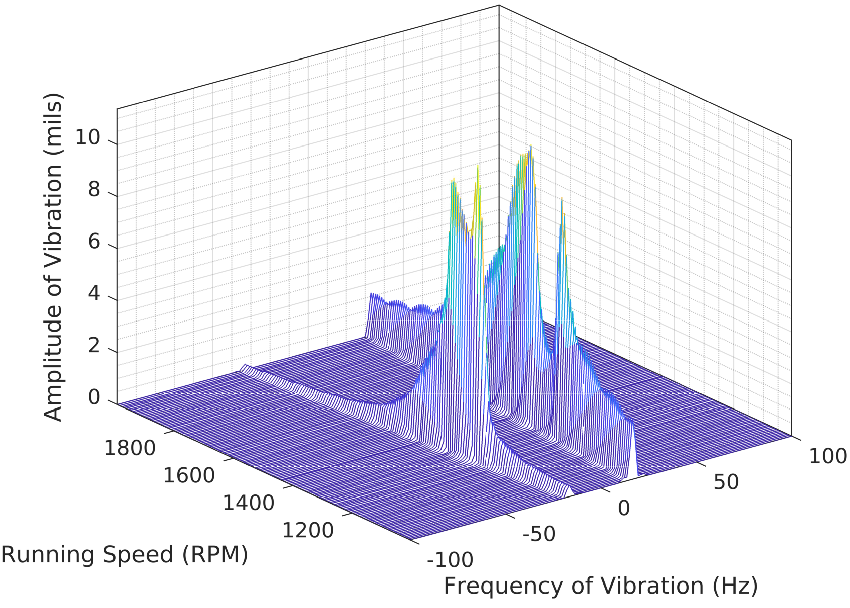
\includegraphics[width=\linewidth]{./figures/ExpExampleCascade2.pdf}
	\caption{Cascade of the experimental system witha synchronous filter applied.}
	\label{fig:ExpExampleCascade2}
\end{figure}
\chapter{Finite Element Method For Rotordynamic systems}
In this chapter the Finite Element Method(FEM) will be employed in the simulation of rotordynamic systems. There are many advantages to using this discretizing method to solve problems of rotating machines. One of which is the generic form that the equation, and its parts take. The method lends itself to being able to easily create new matrices that can insert right into your equations of motion. Another, is the ability to move components around in space without the need to reevaluate the physics. Finally, the analysis techniques for Multiple Degree Of Freedom (MDOF) systems is wide reaching, and will serve to richly enhance our understanding of a complex system made of simple parts.\par 
First, the beam element commonly refered to as the Timoshenko Beam Element will be derived from the kinematic and constitutive constraints (An alternative element, the Bernoulli-Euler element is provided in Appendix A). Then the solution to the resulting equation of motion will be discretized and variables separated in position and time to give the finite element equations of motion. Further, an extension to the beam element model is presented that will consider the viscous damping effects in the beam element. Equations for disks, bearings, and complex versions of all equations will be presented. Finally, the assembly and analysis of the model will result in intuitive figures that will be shown to compare well to experimental data.
\section{Beam Element FE Equation} \label{Beam Element FE Equation}
\subsection{Timoshenko Beam Finite Element} \label{Timoshenko Beam Finite Element}
The Timoshenko beam element allows for the beam cross section plane at any axis location to differ from normal with the axis of the beam. In other words, the element allows for shear stresses. This element often also includes the effects of rotary inertia and gyroscopic moments, as it will in this derivation. Generalized displacements used are assumed to be variable in both time and space. The element has six degrees of freedom. Three translation and three rotations all defined on the beam axis. So then all displacements are functions of time, $ t $, and the axial spacial coordinate, $ x $.
\subsubsection{Kinematic Relationships} \label{Kinematic Relationships}
\begin{figure}
	\centering
	\def\svgwidth{400pt}
	\import{figures/}{kinematicbeamsurface.pdf_tex}
	\caption{Beam Element with nodal displacements.}
	\label{fig:KineBeamElem}
\end{figure}
\begin{figure}
	\centering
	\def\svgwidth{250pt}
	\import{figures/}{TimoBeamDOF.pdf_tex}
	\caption{Timoshenko beam section with degrees of freedom at some point x along beam axis.}
	\label{fig:TimoBeamDOF}
\end{figure}
In order to develop the stresses and strains internal to the beam, and subsequently the equations of motion, the motion of some arbitrary point on the beam must be defined in terms of the generalized coordinates. Motion of two points is taken into consideration to assist in dividing the motion into a translation and a rotation. These points are shown in Figure \ref{fig:KineBeamElem}. The first point, $ C $, falls on the beam axis at location x, and in the undeformed configuration, the vector $ \vec{r}_c^\prime= \overrightarrow{OC} $ forms a right angle with the surface of the cross section. The second point, $ P $ is at some arbitrary $ (y,z) $ location on the cross section. The vecor $ \vec{t}=\overrightarrow{CP} $ points from the beam axis to the point along the cross section. If we follow this point $ P $ we will be able to define the motion of the cross section as a whole, or more succinctly, to define the displacements $ u_p,v_p,w_p $ in terms of the coordinates $ u,v,w,\psi,\theta$, \& $\phi $. The motion of point P is split into translation and rotation, where $ \vec{t} $ is rotated and $ \vec{r}_c $ is translated to point to the deformed location $ P' $. The vector pointing to P in the undeformed state is defined as
\begin{equation}\label{eq:r}
\vec{r}=\vec{r}_c+\vec{t}
\end{equation}
Rotations are represented with a rotation transformation matrix,
\begin{equation}\label{eq:trot}
\vec{t}^\prime=\underline{R}\vec{t}
\end{equation}
The linearized first order rotational matrix for small angles is represented by 
\begin{equation}\label{eq:RotTransformation}
\underline{R}=\left[\begin{array}{ccc}
1&-\theta&\psi\\
\theta&1&-\phi\\
-\psi&\phi&1
\end{array}\right]
\end{equation}
and the translation with a displacement vector 
\begin{equation}\label{eq:rtrans}
\vec{r}_c^\prime=\vec{r}_c+\vec{u}
\end{equation}
%\begin{equation}\label{eq:RotTransformationExpanded}
%R=\underline{I}+\tilde{\underline{\Psi}}+1/2\left(\tilde{\underline{\Psi}}\right)^2+...
%\end{equation}
%\begin{equation}\label{eq:RotTransformationApprox}
%R\approx\underline{I}+\tilde{\underline{\Psi}}
%\end{equation}
Combined motion from $ P $ to $ P' $ can be defined by
\begin{equation}\label{eq:DispVectorrpr}
\vec{u}_p=\vec{r^\prime}-\vec{r}
\end{equation}
where $ \vec{u}_p  $ is the vector containing $ u_p,\:v_p,\:\&\:w_p $. The vector definitions for $ \vec{r}' $ and $ \vec{r} $ are substituted to the above equation to obtain
\begin{equation}\label{eq:DispVectorrptprt}
\vec{u}_p=\vec{r_c^\prime}+\vec{t^\prime}-\vec{r}_c+\vec{t}
\end{equation}
and now using the definition for $ \vec{u} $ and $ \vec{t}' $ leads to the simplified expression for the motion of $ P $
\begin{equation}\label{eq:DispVectRotTranst}
\vec{u}_p=\vec{u}+(\underline{R}-\underline{I})\vec{t}
\end{equation}
expanding matrices reveals the equation
\begin{equation}\label{DispVectExpanded}
\vec{u}_p = \left\{\begin{array}{c}
	u_p\\
	v_p\\
	w_p\end{array}\right\}=\left\{\begin{array}{c}
	u\\
	v\\
	w\end{array}\right\}+\left[\begin{array}{ccc}
	0&-\theta&\psi\\
	\theta&0&-\phi\\
	-\psi&\phi&0
	\end{array}\right]\left\{\begin{array}{c}
	0\\
	y\\
	z\end{array}\right\}
\end{equation}
Therefore, the motion of any point on the beam may be approximated with
\begin{equation}\label{eq:DispVectEvaluated}
\vec{u}_p=\left\{\begin{array}{c}
u-\theta y+\psi z\\
v-\phi z\\
w+\phi y\end{array}\right\}
\end{equation}
\subsubsection{Internal Constitutive Relationship} \label{Internal Constitutive Relationship}
Stresses are assumed to exist in the beam in the axial direction, and in shear on the face of the beam section. Stresses in the transverse, or the y and z, directions are assumed negligible. Shear stresses out of the plane section are assumed to be vanishing as the differential element shrinks. Internal damping is to be considered independently from this material constitutive relationship. Written out, these stresses are represented by the matrix
\begin{equation}\label{key}
\sigma_{ij}=\left[\begin{array}{ccc}
\sigma_{xx}&\sigma_{xy}&\sigma_{xz}\\
\sigma_{xy}&0&0\\
\sigma_{xz}&0&0
\end{array}\right]
\end{equation}
using the Hooke's Law for a linear elastic isotropic material, expressed as
\begin{equation}\label{key}
\epsilon_{ij}=\frac{1}{E}[(1+\nu)\sigma_{ij}-\nu\delta_{ij}\sigma_{kk}]
\end{equation}
allows the determination of the stress strain relationship in engineering notation as
\begin{equation}\label{eq:ConstitutiveRelationshipEngineeringNotation}
\left\{\begin{array}{c}
\sigma_{xx}\\ \sigma_{xy}\\ \sigma_{xz}
\end{array}\right\} = \left[\begin{array}{ccc}
E&0&0\\0&2G&0\\0&0&2G
\end{array}\right] \left\{\begin{array}{c}
\epsilon_{xx}\\ \epsilon_{xy}\\ \epsilon_{xz}
\end{array}\right\}
\end{equation}
where, $ G=\frac{E}{2(1+\nu)} $. Strains are derived from displacements of equation \eqref{eq:DispVectEvaluated} using a linear strain-displacement relationship for infinitesimal strains: $ 2\epsilon_{ij}=u_{i,j}+u_{j,i} $.
%\begin{equation}\label{eq:LinearStrainDispRelationship}
%
%\end{equation}
%\begin{equation}\label{eq:StrainEvaluated}
%\underline{\epsilon}=\frac{1}{2}\left[\begin{array}{ccc}
%2\left(\frac{\partial u_c}{\partial x}-\frac{\partial\theta}{\partial x}y+\frac{\partial\psi}{\partial x}z\right) & \frac{\partial v_c}{\partial x}-\frac{\partial\phi}{\partial x}z-\theta & \frac{\partial w_c}{\partial x}+\frac{\partial \phi}{\partial x}y+\psi\\
%\frac{\partial v_c}{\partial x}-\frac{\partial\phi}{\partial x}z-\theta &0&0\\
%\frac{\partial w_c}{\partial x}+\frac{\partial \phi}{\partial x}y+\psi&0&0\end{array}\right]
%\end{equation}
\begin{equation}\label{eq:StrainEvaluatedSimple}
\left\{\arraycolsep=1pt\begin{array}{rl}
\epsilon_{xx}&=u'-\theta'y+\psi'z\\
\epsilon_{xy}&=\frac{1}{2}(v'-\phi'z-\theta)\\
\epsilon_{xz}&=\frac{1}{2}(w'+\phi'y+\psi)
\end{array}\right.
\end{equation}
Note that in the case of the Euler-Bernoulli beam derivation the slope in a transverse direction displacement is equal to the rotation angle about the orthogonal transverse axis, i.e., $v'=\theta$ and $w'=\psi$. Application of those would reduce the system to the Euler-Bernoulli beam.\par

It will be proven useful to introduce generalized strains that group strain contributions above as axial, bending, torsion, and shear, represented by the symbols $ \varepsilon $, $ \rho $, $ \varphi $, $ \gamma $,respectively.
\begin{equation}\label{eq:GeneralizedStrains}
\left\{\arraycolsep=1pt\begin{array}{rl}
\varepsilon&=u'\\
\rho_{y}&=-\theta'\\
\rho_{z}&=\psi'\\
\varphi&=\phi'\\
\gamma_{y}&=v'-\theta\\
\gamma_{z}&=w'+\psi\end{array}\right.
\end{equation}
allowing the representation of the strains from eq \eqref{eq:StrainEvaluatedSimple} using the generalized strains as:
\begin{equation}\label{eq:StrainEvaluatedSimpleGeneralized}
\left\{\begin{array}{l}
\epsilon_{xx}=\varepsilon+\rho_yy+\rho_zz\\
\epsilon_{xy}=\frac{1}{2}(\gamma_y-\varphi z)\\
\epsilon_{xz}=\frac{1}{2}(\gamma_z+\varphi y)
\end{array}\right.
\end{equation}
Now the stresses in equation \eqref{eq:ConstitutiveRelationshipEngineeringNotation} can be represented with the displacements as 
\begin{equation}\label{key}
\left\{\begin{array}{c}
\sigma_{xx}\\ \sigma_{xy}\\ \sigma_{xz}
\end{array}\right\} = \left\{\begin{array}{c}
E(u'-\theta'y+\psi'z)\\ G(v'-\phi'z-\theta)\\ G(w'+\phi'y+\psi)
\end{array}\right\} = \left\{\begin{array}{c}
E(\varepsilon+\rho_yy+\rho_zz)\\ G(\gamma_y-\varphi z)\\ G(\gamma_z+\varphi y)
\end{array}\right\}
\end{equation}
%Stress at the beam axis is expressed using Hooke's Law for linear isotropic homogeneous material
%\begin{equation}\label{LinearElasticStressStrainRelationship}
%\sigma_{ij}=\lambda\delta_{ij}\epsilon_{kk}+2\mu\epsilon_{ij}
%\end{equation}
%expanded out 
%\begin{equation}\label{StressEvaluated}
%\underline{\sigma}=\left[\begin{array}{ccc}
%(\lambda+2\mu)(u'-\theta'y+\psi'z)&\mu(v'-\phi'z-\theta)&\mu(w'+\phi'y+\psi)\\
%\mu(v'-\phi'z-\theta)&\lambda(u'-\theta'y+\psi'z)&0\\
%\mu(w'+\phi'y+\psi)&0&\lambda(u'-\theta'y+\psi'z)
%\end{array}\right]
%\end{equation}
%\begin{equation}\label{key}
%\sigma_{ij}=\lambda\delta_{ij}\epsilon_{k,k}+\mu\left(u_{i,j}+u_{j,i}\right)
%\end{equation}
\begin{equation}\label{eq:TotalVirtualStrainEnergyExpression}
U = \int_{\volume}\sigma_{ij}\epsilon_{ij}d\volume
\end{equation}
Now the inner product of the total virtual strain energy can be expanded
\begin{equation}\label{eq:TotalStrainEnergyExpanded}
U=\int_{\volume}\left[\sigma_{xx}\epsilon_{xx}+2\sigma_{xy}\epsilon_{xy}+2\sigma_{xz}\epsilon_{xz}\right]d\volume
\end{equation}
Then expand virtual strains into the generalized strains corresponding to the degrees of freedom of the beam element and collect terms on generalized strains
\begin{equation}\label{eq:TotalStrainEnergyGeneralized}
 U=\int_{\volume}\left[\sigma_{xx}\varepsilon+\sigma_{xx}y\rho_y+\sigma_{xx}z\rho_z+\sigma_{xy}\gamma_y+\sigma_{xz}\gamma_z+(\sigma_{xz}y-\sigma_{xy}z)\varphi\right]d\volume
\end{equation}
this internal mechanical energy expression allows us to recognize stresses conjugate with each generalized strain as the corresponding stress for that phenomena. Integration allows the determination of the forces and moments related to each generalized strain as
\begin{equation}\label{eq:generalizedForces}
\left\{\arraycolsep=1pt\begin{array}{rcl}
N=&\int_A\sigma_{xx}dA&=E( A\varepsilon+S_y\rho_y+S_z\rho_z)\\
M_y=&\int_A\sigma_{xx}zdA&=E(S_z\varepsilon+I_{xy}\rho_y+I_y\rho_z)\\
M_z=&\int_A\sigma_{xx}ydA&=E(S_y\varepsilon+I_z\rho_y+I_{xy}\rho_z)\\
Q_y=&\int_A\sigma_{xy}dA&=\kappa G(A\gamma_y-S_z\varphi)\\
Q_z=&\int_A\sigma_{xz}dA&=\kappa G(A\gamma_z+S_y\varphi)\\
M_x=&\int_A(\sigma_{xz}y-\sigma_{xy}z)dA&=\kappa G\left(A_y\gamma_z-A_z\gamma_y+J_x\varphi\right)
\end{array}\right.
\end{equation}
\begin{center}where, $ \left\{\begin{array}{l}
\ \kappa=\frac{6(1+\nu)}{7+6\nu}, \textit{for circular cross sections.}\\
\arraycolsep=.75pt\begin{array}{rlccccrl}
A&=\int_AdA&&&&&S_y&=\int_A ydA\\
S_z&=\int_AzdA&&&&&I_y&=\int_Az^2dA\\
I_z&=\int_Ay^2dA&&&&&J_x&=I_y+I_z
\end{array}
\end{array}\right. $\\\end{center}
$ \kappa $ is the shear coefficient which attempts to correct for the fact that the shear strain is not constant over the beam cross section. Assuming the central axis of the beam is coincident with the shear center, then $ A_y=A_z=I_{xy}=0 $. Which simplifies the conjugate forces to


\begin{equation}\label{eq:generalizedForcesSimplified}
\left\{\arraycolsep=1pt\begin{array}{rll}
N&=EA\varepsilon&=EAu'\\
M_y&=EI_y\rho_z&=EI_y\psi'\\
M_z&=EI_z\rho_y&=-EI_z\theta'\\
Q_y&=\kappa G A\gamma_y&=\kappa G A(v'-\theta)\\
Q_z&=\kappa G A\gamma_z&=\kappa G A(w'+\psi)\\
M_x&=\kappa G J_x\varphi&=\kappa G J_x\phi'
\end{array}\right.
\end{equation}

%\begin{equation}\label{eq:TotalVirtualStrainEnergyGeneralizedExpanded}
%\delta U=\int_{0}^{l}\left[N\delta\varepsilon+M_z\delta\rho_y+M_y\delta\rho_z+Q_y\delta\gamma_y+Q_z\delta\gamma_z+M_x\delta\varphi\right]dx
%\end{equation}
%upon expanding with forces defined in eq \eqref{eq:generalizedForcesSimplified}
%\begin{multline}
%\delta U=\int_{0}^{l}[EAu'\delta u'
%+EI_y\psi'\delta\psi'
%+EI_z\theta'\delta\theta'
%+\kappa G A(v'-\theta)(\delta v'-\delta\theta)\\
%+\kappa G A(w'+\psi)(\delta w'+\delta\psi)
%+\kappa G J_x\phi'\delta\phi']dx
%\end{multline}
%and using integration by parts to achieve a relation to the displacements 
%\begin{multline}\label{eq:TotalVirtualStrainEnergyDisplacementRel}
%\delta U=\int_{0}^{l}\{EAu''\delta u
%+\kappa G A(v''-\theta')\delta v
%+\kappa G A(w''+\psi')\delta w\\
%+[EI_y\psi''-\kappa G A(w'+\psi)]\delta\psi
%+[EI_z\theta''+\kappa G A(v'-\theta)]\delta\theta\\
%+\kappa G J_x\phi''\delta\phi\}dx + \delta U_b
%\end{multline}
%leaving $ \delta U_b $ as the boundary value terms to be neglected. The principle of virtual work for a quasistatic beam with no external work gives $ \delta U=0 $. Therefore, each term in the integrand of \eqref{eq:TotalVirtualStrainEnergyDisplacementRel} must equal zero.
\subsubsection{Differential Equations of Motion} \label{Differential Equations of Motion}
Now the equations are motion are derived for the Timoshenko beam element. External forces are not included in this derivation. Though they may easily be added to the diagram of figure \ref{fig:BeamDifferentialSection} and included in the analysis. It is also assumed that the cross section remains planar during deformation and the material properties are homogeneous through time and space. The derivation is the same as for a Euler-Bernoulli beam with the exception of the constitutive relations used at the end and the inclusion of torsion and axial degrees of freedom.
\begin{figure}
	\centering
	\def\svgwidth{600pt}
	\import{figures/}{BeamDifferentialSection.pdf_tex}
	\caption{Beam differential element with generalized forces.}
	\label{fig:BeamDifferentialSection}
\end{figure}
Using conservation of momentum and conservation of the moment of momentum a relationship between inertia and internal forces is developed. Applying summation of forces in the x-direction
\begin{equation}\label{key}
(N+\frac{1}{2}\frac{\partial N}{\partial x}dx)-(N-\frac{1}{2}\frac{\partial N}{\partial x}dx)=\rho A dx \frac{\partial^2u}{\partial x^2}
\end{equation}
by Simplifying the above equation, and performing the same steps for the other directions and moments we get
\begin{equation}\label{eq:EquilibriumEquations}
\left\{\arraycolsep=1pt\begin{array}{rl}
\frac{\partial N}{\partial x}&=\rho A\frac{\partial^2 u}{\partial x^2}\\
\frac{\partial Q_y}{\partial x}&=\rho A\frac{\partial^2 v}{\partial x^2}\\
\frac{\partial Q_z}{\partial x}&=\rho A\frac{\partial^2 w}{\partial x^2}\\
\frac{\partial M_y}{\partial x}-Q_z&=\rho I_y \frac{\partial^2\psi}{\partial x^2} + \rho J_x\Omega\frac{\partial\theta}{\partial x}\\
\frac{\partial M_z}{\partial x}+Q_y&=\rho I_z \frac{\partial^2\theta}{\partial x^2} - \rho J_x\Omega\frac{\partial\psi}{\partial x}\\
\frac{\partial M_x}{\partial x}&=\rho J_x\frac{\partial^2\phi}{\partial x^2}
\end{array}\right.
\end{equation}
Gyroscopic moments have been explicitly added to the summations in the appropriate equations. The generalized forces of equation \eqref{eq:generalizedForcesSimplified} are substituted in the equilibrium equations \eqref{eq:EquilibriumEquations}
%\begin{equation}\label{eq:EquationsOfMotionIndependent}
%\left\{\arraycolsep=1pt\begin{array}{rl}
%EAu''&=\rho A\ddot{u}\\
%\kappa GA(v''-\theta')&=\rho A\ddot{v}\\
%\kappa GA(w''+\psi')&=\rho A\ddot{w}\\
%EI_y\psi''-\kappa GA(w'-\theta)&=\rho I_y\ddot{\psi}+\rho J_x\Omega\dot{\theta}\\
%EI_z\theta''+\kappa GA(v'+\psi)&=\rho I_z\ddot{\theta}-\rho J_x\Omega\dot{\psi}\\
%\kappa GJ_z\phi''&=\rho J_x\ddot{\phi}
%\end{array}\right.
%\end{equation}
\begin{subequations}\label{eq:EquationsOfMotionIndependent}
\begin{empheq}[left={\empheqlbrace\,}]{align}
EAu''&=\rho A\ddot{u}\label{eq:EquationsOfMotionIndependent_u}\\
\kappa GA(v''-\theta')&=\rho A\ddot{v}\label{eq:EquationsOfMotionIndependent_v}\\
\kappa GA(w''+\psi')&=\rho A\ddot{w}\label{eq:EquationsOfMotionIndependent_w}\\
EI_y\psi''-\kappa GA(w'+\psi)&=\rho I_y\ddot{\psi}+\rho J_x\Omega\dot{\theta}\label{eq:EquationsOfMotionIndependent_psi}\\
EI_z\theta''+\kappa GA(v'-\theta)&=\rho I_z\ddot{\theta}-\rho J_x\Omega\dot{\psi}\label{eq:EquationsOfMotionIndependent_theta}\\
\kappa GJ_x\phi''&=\rho J_x\ddot{\phi}\label{eq:EquationsOfMotionIndependent_phi}
\end{empheq}
\end{subequations}
In matrix form, this system of equations can be represented by this equation
\begin{equation}\label{key}
\bunderline{\mathcal{M}}^e\ddot{\vec{\mathbf{u}}}+\Omega\bunderline{\mathcal{G}}^e\dot{\vec{\mathbf{u}}}-\left(\frac{\partial ()}{\partial x}\bunderline{\mathcal{S}}^e-\bunderline{\mathcal{P}}^e\bunderline{\mathcal{S}}^e\right)\vec{\mathbf{u}}=0
\end{equation}
where,
\begin{equation}\label{key}
\def\cs{2em}
\def\csn{3em}
\newcommand{\SetToWidest}[1]{\makebox[\cs]{$#1$}}%
\left\{\def\arraystretch{1}\arraycolsep=1pt\begin{array}{@{}rlrl}
\bunderline{\mathcal{M}}^e&=\!\left[\def\arraystretch{.8}\arraycolsep=-.5pt\begin{array}{cccccc}
\SetToWidest{\rho A}&\SetToWidest{0}&\SetToWidest{0}&\SetToWidest{0}&\SetToWidest{0}&\SetToWidest{0}\\
0&\rho A&0&0&0&0\\
0&0&\rho I_y&0&0&0\\
0&0&0&\rho I_z&0&0\\
0&0&0&0&\rho A&0\\
0&0&0&0&0&\rho J_x
\end{array}\right]&\bunderline{\mathcal{G}}^e&=\!\left[\def\arraystretch{.8}\arraycolsep=-.5pt\begin{array}{cccccc}
\makebox[\cs]{0}&\makebox[\cs]{0}&\makebox[\cs]{0}&\makebox[\cs]{0}&\makebox[\cs]{0}&\makebox[\cs]{0}\\
0&0&0&0&0&0\\
0&0&0&\rho J_x&0&0\\
0&0&-\rho J_x&0&0&0\\
0&0&0&0&0&0\\
0&0&0&0&0&0
\end{array}\right]\\
&&\\[-1em]
\bunderline{\mathcal{P}}^e&=\!\left[\def\arraystretch{.8}\arraycolsep=-.5pt\begin{array}{cccccc}
\SetToWidest{0}&\SetToWidest{0}&\SetToWidest{0}&\SetToWidest{0}&\SetToWidest{0}&\SetToWidest{0}\\
0&0&0&0&0&0\\
0&1&0&0&0&0\\
-1&0&0&0&0&0\\
0&0&0&0&0&0\\
0&0&0&0&0&0
\end{array}\right]&\bunderline{\mathcal{S}}^e&=\!\left[\def\arraystretch{.8}\arraycolsep=-1pt\begin{array}{@{}cccccc@{}}
\makebox[\csn]{$\kappa GA \frac{\partial ()}{\partial x}$}&\makebox[\csn]{0}&\makebox[\csn]{0}&\makebox[\csn]{$-\kappa G A$}&\makebox[\csn]{0}&\makebox[\csn]{0}\\
0&\kappa GA\frac{\partial ()}{\partial x}&\kappa GA&0&0&0\\
0&0&EI_y\frac{\partial ()}{\partial x}&0&0&0\\
0&0&0&EI_z\frac{\partial ()}{\partial x}&0&0\\
0&0&0&0&EA\frac{\partial ()}{\partial x}&0\\
0&0&0&0&0&\kappa GJ_x\frac{\partial ()}{\partial x}
\end{array}\right]
\end{array}\right.
\end{equation}
and $ \vec{\mathbf{u}}=[v,w,\psi,\theta,u,\phi]^{\T} $ The principle of virtual displacements is utilized on the equations of motion to obtain the weak for of the equations of motion and integrated over the length of the beam.
\begin{equation}\label{eq:BeamDiffEquationVirtualStart}
\int_0^l \delta\vec{\mathbf{u}}^\T\bunderline{\mathcal{M}}^e\ddot{\vec{\mathbf{u}}}dx+\int_0^l \delta\vec{\mathbf{u}}^\T\Omega\bunderline{\mathcal{G}}^e\dot{\vec{\mathbf{u}}}-\int_0^l\delta\vec{\mathbf{u}}^\T\frac{\partial ()}{\partial x}\bunderline{\mathcal{S}}^e\vec{\mathbf{u}}dx+\int_0^l\delta\vec{\mathbf{u}}^\T\bunderline{\mathcal{P}}\bunderline{\mathcal{S}}^e\vec{\mathbf{u}}dx=0
\end{equation}
integration by parts on the third term and replacing $ \underline{\mathcal{S}} $ with $ \bunderline{\mathcal{D}}^e\bunderline{\mathcal{B}} $, and making use of the Identity matrix, $ \bunderline[2]{\mathbf{I}} $ where $ \frac{\partial()}{\partial x}\bunderline{\mathbf{I}} $ is interpreted here as if the partial was a scalar
\begin{equation}\label{key}
\int_0^l \delta\vec{\mathbf{u}}^\T\bunderline{\mathcal{M}}^e\ddot{\vec{\mathbf{u}}}dx+\Omega\int_0^l \delta\vec{\mathbf{u}}^\T\bunderline{\mathcal{G}}^e\dot{\vec{\mathbf{u}}}+\int_0^l\delta\vec{\mathbf{u}}^\T\left(\frac{\partial ()}{\partial x}\bunderline[2]{\mathbf{I}}+\bunderline{\mathcal{P}}\right)\bunderline{\mathcal{D}}^e\bunderline{\mathcal{B}}\vec{\mathbf{u}}dx=0
\end{equation}
\begin{equation}\label{key}
\def\cs{1.5em}
\bunderline{\mathcal{D}}^e=\left[\def\arraystretch{.8}\arraycolsep=1.8pt\begin{array}{cccccc}
\makebox[\cs]{$\kappa GA$}&\makebox[\cs]{0}&\makebox[\cs]{0}&\makebox[\cs]{0}&\makebox[\cs]{0}&\makebox[\cs]{0}\\
0&\kappa GA&0&0&0&0\\
0&0&EI_y&0&0&0\\
0&0&0&EI_z&0&0\\
0&0&0&0&EA&0\\
0&0&0&0&0&\kappa GJ_x
\end{array}\right] \&\quad \bunderline{\mathcal{B}}=\left[\def\arraystretch{.8}\arraycolsep=1.8pt\begin{array}{cccccc}
\makebox[\cs]{$\frac{\partial ()}{\partial x}$}&\makebox[\cs]{0}&\makebox[\cs]{0}&\makebox[\cs]{-1}&\makebox[\cs]{0}&\makebox[\cs]{0}\\
0&\frac{\partial ()}{\partial x}&1&0&0&0\\
0&0&\frac{\partial ()}{\partial x}&0&0&0\\
0&0&0&\frac{\partial ()}{\partial x}&0&0\\
0&0&0&0&\frac{\partial ()}{\partial x}&0\\
0&0&0&0&0&\frac{\partial ()}{\partial x}
\end{array}\right]
\end{equation}
Notice that $ \frac{\partial ()}{\partial x}\bunderline{I}+\bunderline{\mathcal{P}}=\bunderline{\mathcal{B}}^\T $ so the equation of motion becomes
\begin{equation}\label{eq:EquationOfMotionVirtual}
\int_0^l \delta\vec{\mathbf{u}}^\T\bunderline{\mathcal{M}}^e\ddot{\vec{\mathbf{u}}}dx+\Omega\int_0^l \delta\vec{\mathbf{u}}^\T\bunderline{\mathcal{G}}^e\dot{\vec{\mathbf{u}}}+\int_0^l\delta\vec{\mathbf{u}}^\T\bunderline{\mathcal{B}}^\T\bunderline{\mathcal{D}}^e\bunderline{\mathcal{B}}\vec{\mathbf{u}}dx=0
\end{equation}
$ \bunderline{\mathcal{M}}^e $ is the inertia of the element, $ \bunderline{\mathcal{G}}^e $ is the rotating inertia, $ \bunderline{\mathcal{D}}^e $ is the material stress-strain relationship, and $ \bunderline{\mathcal{B}}^e $ is the strain-displacement operator. The solution of this differential system motivates a separation of variables that will be discussed in the next section.
\subsubsection{Shape Functions} \label{Shape Functions}
The displacements thus far have been assumed to be functions of both position and time. Now the total displacement is separated into functions that depend on time and functions that depend on position. This is a fundamental part of the discretization of the beam element, and the use the finite element method. 
\begin{equation} \label{eq:FEGoverning}
\left\{\begin{array}{rl}
\vec{\mathbf{u}}(x,t)&=\bunderline{\mathbf{N}}(x)\vec{\mathbf{q}}(t)\\
\dot{\vec{\mathbf{u}}}(x,t)&=\bunderline{\mathbf{N}}(x)\dot{\vec{\mathbf{q}}}(t)\\
\ddot{\vec{\mathbf{u}}}(x,t)&=\bunderline{\mathbf{N}}(x)\ddot{\vec{\mathbf{q}}}(t)\\
\delta\vec{\mathbf{u}}(x,t)&=\bunderline{\mathbf{N}}(x)\delta\vec{\mathbf{q}}(t)
\end{array}\right.
\end{equation}
where, $ \vec{\mathbf{u}}=[v,w,-\psi,\theta,u,\phi]^\T $ \& $ \vec{\mathbf{q}}=[v_1,w_1,-\psi_1,\theta_1,v_2,w_2,-\psi_2,\theta_2,u_1,\phi_1,u_2,\phi_2]^\T $. This specfic order of $ \vec{\mathbf{q}} $ is chosen with $ u $ and $ \phi $ at the end to ease the condensation of the axial and torsional degrees of freedom out of the system if their use is not necessary for the system of interest. $ \psi $ angles are defined as negative to allow for the same stiffness matrix to define the motion in both planes, and more importantly, to allow for the use of the complex plane to simplify the problem. The shape functions $ \bunderline{\mathbf{N}}(x) $ interpolate the displacements between the beam ends. These functions must must solve the static portion of the differential equations \eqref{eq:EquationsOfMotionIndependent}.
%\begin{subequations}\label{eq:EulerLagrangianEquations}
%	\begin{empheq}[left={\empheqlbrace\,}]{align}
%	&EAu''=0 \label{eq:EulerLagrangianAxial}\\
%	&\kappa GA(v''-\theta')=0 \label{eq:EulerLagrangianSheary}\\
%	&\kappa GA(w''+\psi')=0 \label{eq:EulerLagrangianShearz}\\
%	&\tilde{E}I_y\psi''-\kappa G A(w'+\psi)=0 \label{eq:EulerLagrangianBendingy}\\
%	&\tilde{E}I_z\theta''+\kappa G A(v'-\theta)=0 \label{eq:EulerLagrangianBendingz}\\
%	&\kappa G J_x\phi''=0 \label{eq:EulerLagrangianTorsion}
%	\end{empheq}
%\end{subequations}
%These are the governing differential equations for a Timoshenko beam element.
\begin{figure}
	\centering
	\def\svgwidth{400pt}
	\import{figures/}{BeamElement.pdf_tex}
	\caption{Beam Element with nodal displacements.}
	\label{fig:BeamElem}
\end{figure}
These shape functions are chosen as a polynomials that satisfy the boundary nodal displacements and rotations at the ends of a beam element. These nodal degrees of freedom, depicted in Figure \ref{fig:BeamElem} are considered to be interpolated through the beam element by the shape functions. Interpolation functions chosen are listed in Equation \eqref{eq:DisplacementInterpolationFunctionsChosen}. Axial displacement, $ u $, and torsional rotation, $ \phi $ are independent, so their shape functions are chosen as polynomials that satisfy the differential equation. Conversely, transverse displacements, $ v $ \& $ w $, and bending rotations, $ \psi $ \& $ \theta $ are coupled. Coupling of the shape functions has been proven to reduce some negative effects of linearly interpolated elements \cite{luo2008efficient}. Polynomial functions are chosen for $ v $ \& $ w $ and their rotational counterparts are derived using the differential relations.
\begin{subequations}\label{eq:DisplacementInterpolationFunctionsChosen}
\begin{empheq}[left={\empheqlbrace\,}]{align}
u&=c_1+c_2x \label{eq:AxialInterpolationFunction}\\
v&=c_3+c_4x+c_5x^2+c_6x^3 \label{eq:TransverseyInterpolationFunction}\\ 
w&=c_7+c_8x+c_9x^2+c_{10}x^3 \label{eq:TransversezInterpolationFunction}\\
\phi&=c_{11}+c_{12}x \label{eq:TorsionInterpolationFunction}
\end{empheq}
\end{subequations}
$ c_{1,2,...} $ are the unknown constants of the polynomial solutions. Using transverse displacement of equations \eqref{eq:TransverseyInterpolationFunction} \& \eqref{eq:TransversezInterpolationFunction} in the differential equations \eqref{eq:EquationsOfMotionIndependent_v}, \eqref{eq:EquationsOfMotionIndependent_w}, \eqref{eq:EquationsOfMotionIndependent_psi}, \eqref{eq:EquationsOfMotionIndependent_theta} the interpolation functions of bending rotations are derived as:
\begin{subequations}\label{eq:DisplacmentInterpolationFunctionsDerived}
\begin{empheq}[left={\empheqlbrace\,}]{align}
\psi&=K_yc_{10}-c_8-2c_9x-3c_{10}x^2 \label{eq:RotationyInterpolationFunction}\\
\theta&=K_zc_6+c_4+2c_5x+3c_{6}x^2 \label{eq:RotationzInterpolationFunction}
\end{empheq}
\end{subequations}
where, $ K_y=\frac{6EI_y}{\kappa GA} $\& $ K_z=\frac{6EI_z}{\kappa GA} $
Boundary Conditions
Boundary conditions for the interpolation polynomials of equations \eqref{eq:DisplacementInterpolationFunctionsChosen} \& \eqref{eq:DisplacmentInterpolationFunctionsDerived} are defined as the components of the vector $ \vec{\mathbf{q}} $$ u_j=u(x_j) $ and similarily for other degrees of freedom. Where, $ j=1,2 $ and defines the two states. In this derivation, $ x_1=0 $ and $ x_2=l $. Application of these boundary condition results in this relation between the polynomial constants and the boundary conditions.
\begin{equation}\label{DisplacementInterpolationBoundaryMatrix}
\def\cs{4em}
\newcommand{\WidestEntry}{$\scriptstyle K_y\!-\!3l^2$}%
%\newcommand{\SetToWidest}[1]{\makebox[\widthof{\WidestEntry}]{$#1$}}%
\newcommand{\SetToWidest}[1]{\makebox[\cs]{$#1$}}%
\left\{\def\arraystretch{.8}\begin{array}{@{}c@{}}
u_1\\u_2\\v_1\\v_2\\w_1\\w_2\\\psi_1\\\psi_2\\\theta_1\\\theta_2\\\phi_1\\\phi_2
\end{array}\right\}\hspace{-4pt}=\hspace{-4pt}\left[\arraycolsep=-.68em\def\arraystretch{.8}\begin{array}{@{}lccccccccccr@{}}
\makebox[\cs/2][l]{1}& \SetToWidest{0}& \SetToWidest{0}& \SetToWidest{0}& \SetToWidest{0}& \SetToWidest{0}& \SetToWidest{0}& \SetToWidest{0}& \SetToWidest{0}& \SetToWidest{0}& \SetToWidest{0}& \makebox[\cs/2][r]{0}\\
1& l& 0& 0& 0& 0& 0& 0& 0& 0& 0& 0\\
0& 0& 1& 0& 0& 0& 0& 0& 0& 0& 0& 0\\
0& 0& 1& l& l^2& l^3& 0& 0& 0& 0& 0& 0\\
0& 0& 0& 0& 0& 0& 1& 0& 0& 0& 0& 0\\
0& 0& 0& 0& 0& 0& 1& l& l^2& l^3& 0& 0\\
0& 0& 0& 0& 0& 0& 0& \text{-}1& 0& \text{-}K_y& 0& 0\\
0& 0& 0& 0& 0& 0& 0& \text{-}1& \text{-}2l& \text{-}K_y\text{-}3l^2& 0& 0\\
0& 0& 0& 1& 0&  K_z& 0& 0& 0& 0& 0& 0\\
0& 0& 0& 1& 2l&  K_z\!\text{+}3l^2& 0& 0& 0& 0& 0& 0\\
0& 0& 0& 0& 0& 0& 0& 0& 0& 0& 1& 0\\
0& 0& 0& 0& 0& 0& 0& 0& 0& 0& 1& l
\end{array}\right]\hspace{-6pt}\left\{\def\arraystretch{.8}\begin{array}{@{}c@{}}
c_1\\c_2\\c_3\\c_4\\c_5\\c_6\\c_7\\c_8\\c_9\\c_{10}\\c_{11}\\c_{12}
\end{array}\right\}
\end{equation}
Inversion of this matrix results in a system of equations defining the constant $ c_1 $ through $ c_{12} $. These constants are then substituted in to the polynomial expressions \eqref{eq:DisplacementInterpolationFunctionsChosen} \& \eqref{eq:DisplacmentInterpolationFunctionsDerived} giving the interpolations as functions of the nodal displacements.
\begin{equation}\label{eq:InterpolationFunctions}
\left\{\begin{array}{l}
u=N_1u_1+N_2u_2\\
v=T_{t_1y}v_1+T_{t_2y}v_2+T_{r_1y}\theta_1+T_{r_2y}\theta_2\\
w=T_{t_1z}w_1+T_{t_2w}w_2+T_{r_1z}\psi_1+T_{r_2z}\psi_2\\
\psi=R_{t_1z}w_1+R_{t_2w}w_2+R_{r_1z}\psi_1+R_{r_2z}\psi_2\\
\theta=R_{t_1y}v_1+R_{t_2y}v_2+R_{r_1y}\theta_1+R_{r_2y}\theta_2\\
\phi=N_1\phi_1+N_2\phi_2
\end{array}\right.
\end{equation}
with;
\begin{equation}\label{eq:TimoShapeFunctions}
\left\{\arraycolsep=.2em\begin{array}{@{}ll}
N_1=1-\zeta&N_2=\zeta\\
T_{t_1y,z}=\frac{1}{1+\alpha_{y,z}}(2\zeta^3-3\zeta^2-\alpha_{y,z}\zeta+1+\alpha_{y,z})&T_{t_2y,z}=\frac{1}{1+\alpha_{y,z}}(-2\zeta^3+3\zeta^2+\alpha_{y,z}\zeta)\\
T_{r_1y,z}=\frac{l}{1+\alpha_{y,z}}[\zeta^3-(2+\frac{1}{2}\alpha_{y,z})\zeta^2+(1+\frac{1}{2}\alpha_{y,z})\zeta]&T_{r_2y,z}=\frac{l}{1+\alpha_{y,z}}[\zeta^3-(1-\frac{1}{2}\alpha_{y,z})\zeta^2-\frac{1}{2}\alpha_{y,z}\zeta]\\
R_{t_1y,z}=\frac{6/l}{1+\alpha_{y,z}}(\zeta^2-\zeta)&R_{t_2y,z}=\frac{6/l}{1+\alpha_{y,z}}(-\zeta^2+\zeta)\\
R_{r_1y,z}=\frac{1}{1+\alpha_{y,z}}(3\zeta^2-(4+\alpha_{y,z})\zeta+1+\alpha_{y,z})&R_{r_2y,z}=\frac{1}{1+\alpha_{y,z}}(3\zeta^2-(2-\alpha_{y,z})\zeta)
\end{array}\right.
\end{equation}
where, $ \alpha_y=2K_y/l^2=\frac{12EI_y}{\kappa GAl^2} $, $ \alpha_z=2K_z/l^2=\frac{12EI_z}{\kappa GAl^2} $, \& $ \zeta=x/l $.
\eqref{eq:InterpolationFunctions} is expressed in matrix form as it appears in \eqref{eq:FEGoverning} where
\begin{equation}\label{ShapeFunctionMatrix}
\def\cs{2em}
\bunderline{\mathbf{N}}(x)=\left[\def\arraystretch{.8}\arraycolsep=0em\begin{array}{cccccccccccc}
\makebox[\cs]{$T_{t_1y}$}&\makebox[\cs]{0}&\makebox[\cs]{0}&\makebox[\cs]{$T_{r_1y}$}&\makebox[\cs]{$T_{t_2y}$}&\makebox[\cs]{0}&\makebox[\cs]{0}&\makebox[\cs]{$T_{r_2y}$}&\makebox[\cs]{0}&\makebox[\cs]{0}&\makebox[\cs]{0}&\makebox[\cs]{0}\\
0&T_{t_1z}&T_{r_1z}&0&0&T_{t_2z}&T_{r_2z}&0&0&0&0&0\\
0&R_{t_1z}&R_{r_1z}&0&0&R_{t_2z}&R_{r_2z}&0&0&0&0&0\\
R_{t_1y}&0&0&R_{r_1y}&R_{t_2y}&0&0&R_{r_2y}&0&0&0&0\\
0&0&0&0&0&0&0&0&N_1&0&N_2&0\\
0&0&0&0&0&0&0&0&0&N_1&0&N_2
\end{array}\right]
\end{equation}
still with the generalized displacement vector $ \vec{\mathbf{q}}=[v_1,w_1,-\psi_1,\theta_1,v_2,w_2,-\psi_2,\theta_2,u_1,\phi_1,u_2,\phi_2]^\T $\par
Shape functions depend on the term $ \alpha $ which is sometimes called the shear correction factor. This shear correction factor is proportional to the square of the ratio of radius to length of the beam element. So, as the length increases relative to the radius, $ \alpha $ tends to zero. It will be evident in the following section that as $ \alpha $ approaches zero, the equations of motion approach the equations of the Bernoulli-Euler beam. A spatial representation of the shape functions of equation \eqref{eq:TimoShapeFunctions} is given in figure \ref{fig:ShapeFunctions}.
\begin{figure}[h!]	
	\begin{subfigure}{.5\linewidth}
		\pgfplotsset{every picture/.style={scale=1},every axis/.style={title style={yshift=-.8em}}}%, every axis/.style={hide axis}}%
		\centering
		\import{figures/}{Shapes.tex}
		\caption{length to radius ratio of 100.}
		\label{fig:ShapeFunctions100}
	\end{subfigure}
	\begin{subfigure}{.5\linewidth}
		\pgfplotsset{every picture/.style={scale=1},every axis/.style={title style={yshift=-.8em}}}%, every axis/.style={hide axis}}%
		\centering
		\import{figures/}{Shapes2.tex}
		\caption{length to radius ratio of 1.}
		\label{fig:ShapeFunctions1}
	\end{subfigure}
	\caption{Shape Functions as they vary with $ \zeta $ using two different ratios of length to radius of beam element.}
	\label{fig:ShapeFunctions}
\end{figure}
Shape functions plotted with respect to the non-dimensional length lend a visualization to the contribution of each shape function. Shape functions for axial and torsion are omitted since they are just linear polynomials. Each individual plot can be interpreted as a transformation from the input, being the coordinate multiplied to it, to the output of the variable function. For instance, the first shape function plot is the output of $ v(x) $ with an input of $ v_1 $ while all other coordinates are zero. The shape makes sense under this interpretation, as the translation starts at some value, $ v_1 $ and decreases to zero at the end since $ v_2 $ is zero. Also, the expected shape breaks as the radius approaches the length as in Figure \ref{fig:ShapeFunctions1}. All shapes this beam will make in the model is a linear combination of the shapes shown here.
\subsubsection{Finite Equations of Motion} \label{Finite Equations of Motion}
To obtain the equations of motion in terms of the generalized coordinates, $ \vec{\mathbf{q}} $, displacement variables $ \vec{\mathbf{u}} $ are replaced with definitions in equation \ref{eq:FEGoverning}.
\begin{equation}\label{key}
\int_0^l \bunderline{\mathbf{N}}^\T\delta\vec{\mathbf{q}}^\T\bunderline{\mathcal{M}}^e\bunderline{\mathbf{N}}\ddot{\vec{\mathbf{q}}}dx+\Omega\int_0^l \bunderline{\mathbf{N}}^\T\delta\vec{\mathbf{q}}^\T\bunderline{\mathcal{G}}^e\bunderline{\mathbf{N}}\dot{\vec{\mathbf{q}}}dx+\int_0^l\bunderline{\mathbf{N}}^\T\delta\vec{\mathbf{q}}^\T\bunderline{\mathcal{B}}^\T\bunderline{\mathcal{D}}^e\bunderline{\mathcal{B}}\bunderline{\mathbf{N}}\vec{\mathbf{q}}dx=0
\end{equation}
Note that $ \vec{\mathbf{q}} $ is not dependent on x so it, and it's derivatives, may be pulled out of the integrals. Define $ \bunderline{\mathbf{B}}=\bunderline{\mathcal{B}}\bunderline{\mathbf{N}} $ and substitute in, noting that $ \bunderline{\mathbf{B}} $ interpolates strains from discrete displacements $ \vec{\mathbf{q}} $. The motion equations are then
\begin{equation}\label{eq:GoverningDifferentialEquationDiscrete}
\int_0^l \bunderline{\mathbf{N}}^\T\bunderline{\mathcal{M}}^e\bunderline{\mathbf{N}}dx\ddot{\vec{\mathbf{q}}}+\Omega\int_0^l \bunderline{\mathbf{N}}^\T\bunderline{\mathcal{G}}^e\bunderline{\mathbf{N}}dx\dot{\vec{\mathbf{q}}}+\int_0^l\bunderline{\mathbf{B}}^\T\bunderline{\mathcal{D}}^e\bunderline{\mathbf{B}}dx\vec{\mathbf{q}}=0
\end{equation}
Define 
\begin{subequations}\label{key}
\begin{empheq}[left={\empheqlbrace\,}]{align}
\bunderline{\mathbf{M}}^e&=\int_0^l \bunderline{\mathbf{N}}^\T\bunderline{\mathcal{M}}^e\bunderline{\mathbf{N}}dx\label{eq:ConsistentMassMatrix}\\
\bunderline{\mathbf{G}}^e&=\int_0^l \bunderline{\mathbf{N}}^\T\bunderline{\mathcal{G}}^e\bunderline{\mathbf{N}}dx\label{eq:ConsistentGyroMatrix}\\
\bunderline{\mathbf{K}}^e&=\int_0^l\bunderline{\mathbf{B}}^\T\bunderline{\mathcal{D}}^e\bunderline{\mathbf{B}}dx\label{eq:ConsistentStiffnessMatrix}
\end{empheq}
\end{subequations}
so that, the general equations of motion for the timoshenko beam element are
\begin{equation}\label{eq:EquationsOfMotionTimoElementGeneral}
\bunderline{\mathbf{M}}^e\ddot{\vec{\mathbf{q}}}+\Omega\bunderline{\mathbf{G}}^e\dot{\vec{\mathbf{q}}}+\bunderline{\mathbf{K}}^e\vec{\mathbf{q}}=0
\end{equation}
Notwithstanding the inclusion of viscous and hysteretic internal damping phenomena. Derivations, and inclusion of these phenomena in the equations of motion are to be included in the following section.
\subsubsection{Rotating Internal Damping} \label{Rotating Internal Damping}
Rotating damping is the main cause of instability in rotating machines. Non-rotating damping, such as the damping contributions from bearing supports, introduce a stabilizing effect. But, as rotating damping is dependent on rotation, its direction of force can contribute to destabilization. Typically, friction components such as bearings with shrink fits or oil bearings are responsible for this destabilizing force. Due to the inherent complexity of modeling loose bearing components, or shrink fit dynamics, the analysis of the internal damping in the shaft elements is considered alone. This will allow for the study of the destabilizing effect in general, and the factors that may contribute stability such as structural damping and anisotropy of supports. Another area of interest is the design of components for specific rotor geometry to maximize the stability in the system. This stability analysis is only possible with the inclusion of some destabilizing force, \cite{genta2007dynamics},\cite{genta2004persistent},\cite{kandil2005rotor},\cite{zorzi1977finite}.\par 
To motivate understanding of this force a simple derivation is provided with a rotating damping whose force is proportional to the flex of rate of change of the flex of the shaft. Obviously this is easier to define in the rotating reference frame, as the variables in this coordinate system directly represent the flex of the shaft from its neutral position. This relationship is as follows:
\begin{equation}\label{eq:LinearViscousDampingRot}
\vec{\mathcal{F}}_{\xi\eta}=-c_r
\left\{\begin{array}{c}
\dot{\xi}_c\\
\dot{\eta}_c
\end{array}\right\}
\end{equation}
Now to translate this force back to the stationary reference frame, we will see the rotation transformation matrix 
\begin{equation}\label{eq:RotationTransformation2D}
\bunderline{\mathcal{R}}=\left[\begin{array}{cc}
\cos{\Omega t}& \sin{\Omega t}\\
-\sin{\Omega t}& \cos{\Omega t}
\end{array}\right]
\end{equation}
transforms stationary into rotating coordinates 
\begin{equation}\label{eq:LinRotTransformation}
\left\{\begin{array}{rl}
\left\{\begin{array}{c}
\xi_c\\
\eta_c
\end{array}\right\}&=\bunderline{\mathcal{R}}\left\{\begin{array}{c}
y_c\\
z_c
\end{array}\right\}\\
&\\[-1em]
\left\{\begin{array}{c}
\dot{\xi}_c\\
\dot{\eta}_c
\end{array}\right\}&=\bunderline{\mathcal{R}}\left\{\begin{array}{c}
\dot{y}_c\\
\dot{z}_c
\end{array}\right\}+\dot{\bunderline{\mathcal{R}}}\left\{\begin{array}{c}
y_c\\
z_c
\end{array}\right\}
\end{array}\right.
\end{equation}
where, \begin{equation}
\dot{\bunderline{\mathcal{R}}}=\Omega\left[\begin{array}{cc}
-\sin{\Omega t}& \cos{\Omega t}\\
-\cos{\Omega t}& -\sin{\Omega t}
\end{array}\right]
\end{equation}
substituting the second equation in \ref{eq:LinRotTransformation} for the velocities in \ref{eq:LinearViscousDampingRot}
\begin{equation}\label{eq:LinearViscousDampingTrans}
\vec{\mathcal{F}}_{xy}=-c_r\left\{\begin{array}{c}
\dot{y}_c\\
\dot{z}_c
\end{array}\right\}-c_r\Omega\left[\begin{array}{@{}rc}
0&1\\
-1&0
\end{array}\right]\left\{\begin{array}{c}
y_c\\
z_c
\end{array}\right\}
\end{equation} 
From the equation \eqref{eq:LinearViscousDampingTrans} we see a dependence on both velocity and position. The portion dependent on the velocity is inherently stable as pulls opposite the motion. Conversely, the portion dependent on position cross couples the two displacements. This causes a destabilizing effect that grows as $ \Omega $ increases. A net destabilizing force is produced once the latter portion of the exceeds the former. Without the presence of other structural damping forces, the system will destabilize.\par
For the beam element, the constitutive relationship\cite{zorzi1977finite} is comprised of both viscous and hysteretic forms of damping, $ \eta_v $ \& $ \eta_h $ respectively.
\begin{equation}\label{eq:LinearViscousHystericConstitutiveRelation}
\sigma_{xx}=E\left\{\frac{\epsilon_{xx}}{\sqrt{1+\eta_h^2}}+\left(\eta_v+\frac{\eta_h}{\omega\sqrt{1+\eta_h^2}}\right)\dot{\epsilon}_{xx}\right\}
\end{equation}
through the use of kinematics to obtain strain-displacement relations,
\begin{equation}\label{eq:straindisplacement}
\left\{\begin{array}{rl}
\epsilon_{xx}&=-r\cos{\left(\Omega-\omega \right)t}\frac{\partial^2 R}{\partial x^2}\\
\dot{\epsilon}_{xx}&=(\Omega-\omega)r\sin{(\Omega-\omega)t}\frac{\partial^2 R}{\partial x^2} - r\cos{(\Omega-\omega)t}\frac{\partial}{\partial t}\frac{\partial^2 R}{\partial x^2}
\end{array}\right.
\end{equation}
and inspection to obtain moment equations,
\begin{equation}\label{eq:momentequations}
\left\{\begin{array}{rl}
M_y &= \int_0^{2\pi}\int_0^a[w+r\sin{\Omega t}]\sigma_{xx}dr(rd(\Omega t))\\
M_z &= \int_0^{2\pi}\int_0^a-[v+r\cos{\Omega t}]\sigma_{xx}dr(rd(\Omega t))
\end{array}\right.
\end{equation}
we can complete a moment bending relationship to be used in the equations of motion
\begin{equation}\label{key}
\def\cs{4em}
\def\cd{1.5em}
\left\{\def\arraystretch{.8}\begin{array}{@{}c@{}}
M_y\\
M_z
\end{array}\right\} = E I\left[\def\arraystretch{.8}\arraycolsep=0em\begin{array}{@{}cc@{}}
\makebox[\cs]{$\eta_a$}&\makebox[\cs]{$\Omega \eta_v+\eta_b$}\\
\Omega \eta_v+\eta_b&-\eta_a
\end{array}\right]\left\{\arraycolsep=0pt\def\arraystretch{.8}\begin{array}{@{}c@{}}
v''\\
w''
\end{array}\right\}+EI\left[\arraycolsep=0pt\def\arraystretch{.8}\begin{array}{@{}cc@{}}
\makebox[\cd]{$\eta_v$}&\makebox[\cd]{0}\\
0&-\eta_v
\end{array}\right]\left\{\arraycolsep=0pt\def\arraystretch{.8}\begin{array}{@{}c@{}}
\dot{v}''\\
\dot{w}''
\end{array}\right\}
\end{equation}
where, $ \eta_a=\frac{1+\eta_h}{\sqrt{1+\eta_h^2}}\quad \& \quad \eta_b=\frac{\eta_h}{\sqrt{1+\eta_h^2}} $\par 
Now use the same strategy followed when solving for the weak form of the beam differential equations using the Principle of Virtual Displacements starting at equation \eqref{eq:BeamDiffEquationVirtualStart}. Then use the seperation of variables of defined by equation \eqref{eq:FEGoverning} to arrive at the total beam element equations of motion including internal damping as
\begin{equation}\label{eq:TotalBeamFiniteElementEquationofMotion}
\bunderline{\mathbf{M}}^e\ddot{\vec{\mathbf{q}}}+(\eta_v\bunderline{\mathbf{K}}^e+\Omega\bunderline{\mathbf{G}}^e)\dot{\vec{\mathbf{q}}}+[\eta_a\bunderline{\mathbf{K}}^e+(\Omega\eta_v+\eta_b)\bunderline{\mathbf{C}}^e]\vec{\mathbf{q}}=0
\end{equation}
where,
\begin{equation}\label{key}
\bunderline{\mathcal{I}}=\left[\def\arraystretch{.8}\begin{array}{cccccc}
0&1&0&0&0&0\\
-1&0&0&0&0&0\\
0&0&0&1&0&0\\
0&0&-1&0&0&0\\
0&0&0&0&0&0\\
0&0&0&0&0&0
\end{array}\right]\:\&\:\begin{array}{c}
\bunderline{\mathbf{C}}^e=\int_0^l\bunderline{\mathbf{B}}^\T\bunderline{\mathcal{I}}\bunderline{\mathcal{D}}\bunderline{\mathbf{B}}dx
\end{array}
\end{equation}
$ \bunderline{\mathbf{C}}^e $ is the ``Circulation matrix", or the skew symmetric stiffness matrix.
\subsubsection{Beam Element in Complex Coordinates} \label{Beam Element in Complex Coordinates}
Complex coordinates collapse the equations of each plane into one set of equations. This lends properties to a axisymmetric rotor systems that will be exploited in the analysis of the model. For the complex analysis in this body of work, the system is assumed to be axisymmetric and the torsional and axial degrees of freedom are omitted. Since the contributions from axial and torsional degrees of freedom are uncoupled from the system, there condensation has no effect on the remainder of system matrices. Complex coordinates used here are defined as:
\begin{equation}\label{eq:ComplexCoordinates}
\vec{\mathbf{s}}=\left\{\begin{array}{c}
\vec{r}\\
\vec{p}
\end{array}\right\}=\left\{\begin{array}{c}
v+iw\\
\theta-i\psi\end{array}\right\}
\end{equation}
Because the element is axisymmetric, and the special form of coordinates is used, symmetric beam equations in one plane hold for the complex plane and skew symmetric matrices become complex versions of the same matrix. Elemental matrices can be formed using the collapsed version of the shape functions matrix
\begin{equation}\label{ShapeFunctionMatrixComplex}
\def\cs{2em}
\bunderline{\mathbf{N}}^c=\left[\def\arraystretch{.8}\arraycolsep=0em\begin{array}{cccc}
\makebox[\cs]{$T_{t_1y}$}&\makebox[\cs]{$T_{r_1y}$}&\makebox[\cs]{$T_{t_2y}$}&\makebox[\cs]{$T_{r_2y}$}\\
R_{t_1}&R_{r_1}&R_{t_2}&R_{r_2}
\end{array}\right]
\end{equation}
in 
\begin{equation}\label{eq:FEGoverningComplex}
\vec{\mathbf{s}}=\bunderline{\mathbf{N}}^c\vec{\mathbf{q}}^c
\end{equation}
where $ \vec{\mathbf{q}}^c=[\vec{\mathbf{s}}_1,\vec{\mathbf{s}}_2]^\T $.\par 
To convince this property of the system in the complex plane, a proof for the elemental equations of motion will be made. Taking equation \eqref{eq:EquationsOfMotionIndependent_v}, adding equation \eqref{eq:EquationsOfMotionIndependent_w} multiplied by the imaginary unit $ i $ and using the definition for complex variables $ \vec{p} $ and $ \vec{r} $ leads to the transverse equation of motion in the complex plane
\begin{equation}\label{eq:EquationsOfMotionIndependent_r_complex}
\kappa GA(\vec{r}''-\vec{p}')=\rho A \ddot{\vec{r}}
\end{equation}
and taking equation \eqref{eq:EquationsOfMotionIndependent_theta} and subtracting equation \eqref{eq:EquationsOfMotionIndependent_psi} multiplied by $ i $ gives the rotation equation in the complex plane
\begin{equation}\label{key}
EI\vec{p}''-\kappa GA(\vec{r}'-\vec{p})=\rho I\ddot{\vec{p}}+i\rho J \Omega\dot{\vec{p}}
\end{equation}
which by inspection of both of these equations it is evident that the form is the same as equations \eqref{eq:EquationsOfMotionIndependent_v} and \eqref{eq:EquationsOfMotionIndependent_theta} except for the imaginary unit on the cross coupled parts of the equation. Now that this idea is motivated, the finite element equations of motion analogous to equation \eqref{eq:TotalBeamFiniteElementEquationofMotion} are
\begin{equation}\label{eq:TotalBeamFiniteElementEquationofMotionComplex]}
\bunderline{\mathbf{M}}^{ec}\ddot{\vec{\mathbf{q}}}^c+(\eta_v\bunderline{\mathbf{K}}^{ec}-i\Omega\bunderline{\mathbf{G}}^{ec})\dot{\vec{\mathbf{q}}}^c+[\eta_a\bunderline{\mathbf{K}}^{ec}-i(\Omega\eta_v+\eta_b)\bunderline{\mathbf{C}}^{ec}]\vec{\mathbf{q}}^c=0
\end{equation}
\section{Disk Nodal Equations} \label{Disk Nodal Equations}
Since the beam element has been discretized into nodal degrees of freedom, so long as the locations of disks in the model are chosen to coincide with one of these nodal locations, the expressions for stiffness and inertia can be directly combined with the global matrices at that node. The mass element is considered as a body at a point with inertia, gyroscopic moments, and unbalance considered as external forces.
\begin{equation}\label{eq:DiskNodeEquationofMotion}
\bunderline{\mathbf{M}}^d\ddot{\vec{\mathbf{q}}}_k+\Omega\bunderline{\mathbf{G}}^d\dot{\vec{\mathbf{q}}}_k=\Omega^2\vec{\mathbf{F}}^d
\end{equation}
the superscript $ d $ represents that the matrix or array is for a disk, and the subscript $ _k $ on the displacement array indicates the array is only displacements for a single node, written out as: $ \vec{\mathbf{q}}_k = [v,w,-\psi,\theta,u,\phi]^\T $. The matrices and forcing array of \eqref{eq:DiskNodeEquationofMotion} are as follows,
\begin{equation}\label{eq:DiskNodeEquations}
\def\cs{3em}
\left\{
\begin{array}{@{}c}
\arraycolsep=1pt\begin{array}{rlrl}
\bunderline{\mathbf{M}}^d & =\!\left[\def\arraystretch{.8}\arraycolsep=-.5em\begin{array}{cccccc}
\makebox[\cs]{$\rho Al$}&\makebox[\cs]{0}&\makebox[\cs]{0}&\makebox[\cs]{0}&\makebox[\cs]{0}&\makebox[\cs]{0}\\
0&\rho Al&0&0&0&0\\
0&0&\rho I_{z}&0&0&0\\
0&0&0&\rho I_{y}&0&0\\
0&0&0&0&\rho Al&0\\
0&0&0&0&0&\rho J_x
\end{array}\right] & \bunderline{\mathbf{G}} & = \!\left[\def\arraystretch{.8}\arraycolsep=-.5em\begin{array}{cccccc}
\makebox[\cs]{0}&\makebox[\cs]{0}&\makebox[\cs]{0}&\makebox[\cs]{0}&\makebox[\cs]{0}&\makebox[\cs]{0}\\
0&0&0&0&0&0\\
0&0&0&\rho J_x&0&0\\
0&0&-\rho J_x&0&0&0\\
0&0&0&0&0&0\\
0&0&0&0&0&0
\end{array}\right]\\
\end{array}\\
\\[-1em]
\vec{\mathbf{F}}^d=\left\{\def\arraystretch{.8}\begin{array}{c}
\rho Al\epsilon\cos(\Omega t + \delta_\varepsilon)\\
\rho Al\epsilon\sin(\Omega t + \delta_\varepsilon)\\
-\rho( I_y-J_x)\chi\sin(\Omega t)\\
\rho( I_z-J_x)\chi\cos(\Omega t)\\
0\\
0
\end{array}\right\}
\end{array}\right.
\end{equation}
\begin{figure}
	\centering
	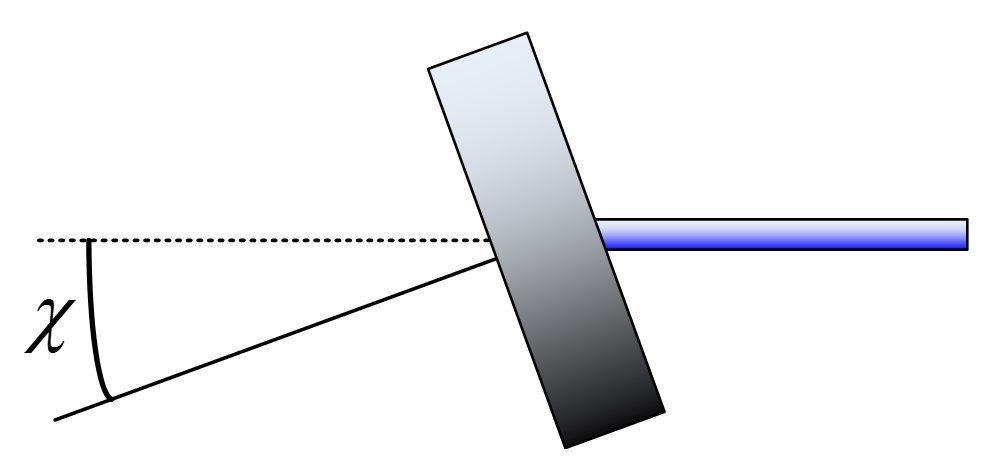
\includegraphics[width=.5\linewidth]{./figures/Images/Figure_1b}
	\caption{Depiction of skew angle $\chi$}
	\label{fig:ChiAngleDepiction}
	\centering
\end{figure}
\par
 Disk unbalance is caused by an eccentricity, or a geometrical distance between the axis of rotation and the center of mass of the disk. Eccentricity is represented here as $\epsilon$ and is equivalent to that geometric distance. The moment unbalance forces, the third and fourth equations of $ \vec{\mathbf{F}}^d $ in \eqref{eq:DiskNodeEquations}, are caused by the skew angle, $ \chi $, which is the angle the disk major axis forms with the axis of rotation as in Figure \ref{fig:ChiAngleDepiction}. The major axis is the axis normal from the disk face from which the polar moment of inertia, $ J_x $ is defined.
 \subsection{Disk in complex coordinates} \label{Disk in complex coordinates}
 Disk equations of motion \eqref{eq:DiskNodeEquationofMotion} are converted to the complex plane in the same manner the beam element was derived in \S\ref{Beam Element in Complex Coordinates}
 \begin{equation}\label{eq:DiskNodeEquationofMotionComplex}
 \bunderline{\mathbf{M}}^{dc}\ddot{\vec{\mathbf{q}}}^c_k-i\Omega\bunderline{\mathbf{G}}^{dc}\dot{\vec{\mathbf{q}}}^c_k=\Omega^2\vec{\mathbf{F}}^{dc}
 \end{equation}
 where,
 \begin{equation*}
 \bunderline{\mathbf{M}}^{dc}=\left[\begin{array}{cc}
 \rho Al&0\\
 0&\rho I
 \end{array}\right],\quad
 \bunderline{\mathbf{G}}^{dc}=\left[\begin{array}{cc}
 0&0\\
 0&\rho J_x
 \end{array}\right],\quad
 \vec{\mathbf{F}}^{dc}=\left\{\begin{array}{c}
 \rho A l \epsilon e^{i\delta_\epsilon}e^{i\Omega t}\\
 \rho(I-J_x)\chi e^{i\Omega t}
 \end{array}\right\}
 \end{equation*}
%\lstinputlisting[language=Matlab]{code/DiskMass.m}
%\lstinputlisting[language=Matlab]{code/DiskGyro.m}
\section{Bearing Nodal Equations} \label{Bearing Nodal Equations}
Bearings in this work are to be considered massless points of stiffness and damping acting at a node. Represented by the local equations of motion
\begin{equation}\label{eq:BearingNodeEquationsofMotion}
\bunderline{\mathbf{D}}^b\dot{\vec{\mathbf{q}}}_k+\bunderline{\mathbf{K}}^b\vec{\mathbf{q}}_k=0
\end{equation}
The superscript $ ^b $ indicates the matrix is for a bearing. A simple model for the stiffness and damping is used. Structural damping of the bearing is considered to be proportional to the stiffness, Raleigh Damping for the local bearing system. The stiffness matrix is comprised of only transverse stiffness terms, as 
\begin{equation}
\def\cs{2em}
\begin{array}{cc}
\bunderline{\mathbf{K}}^b=\left[\def\arraystretch{.8}\arraycolsep=0pt\begin{array}{cccccc}
\makebox[\cs]{$k_{yy}$}&\makebox[\cs]{$k_{yz}$}&\makebox[\cs]{0}&\makebox[\cs]{0}&\makebox[\cs]{0}&\makebox[\cs]{0}\\
k_{zy}&k_{zz}&0&0&0&0\\
0&0&0&0&0&0\\
0&0&0&0&0&0\\
0&0&0&0&0&0\\
0&0&0&0&0&0
\end{array}\right] & \bunderline{\mathbf{D}}^b=a\bunderline{\mathbf{K}}^b
\end{array}
\end{equation}
The stiffness is typically simplified further to represent an orthotropic bearing, where $ k_{yz}=k_{zy}=0 $ or further yet as a isotropic bearing, where $ k_{yz}=k_{zy}=0 $ \& $ k_{yy}=k_{zz}=k $. Generally, these unknown parameters of stiffness are determined by changing the values to achieve the correct natural frequencies of the system.
\subsection{Bearing in Complex Coordinates}
Following the same methodology as sections \S\ref{Beam Element in Complex Coordinates} \& \S\ref{Disk in complex coordinates}, the equation of motion in the complex plane is
\begin{equation}\label{eq:BearingNodeEquationsofMotionComplex}
\bunderline{\mathbf{D}}^{bc}\dot{\vec{\mathbf{q}}}^c_k+\bunderline{\mathbf{K}}^{bc}\vec{\mathbf{q}}^c_k=0
\end{equation}
where,
\begin{equation*}
 \bunderline{\mathbf{K}}^{bc}=\left[\begin{array}{cc}
k&0\\
0&k
\end{array}\right],\quad
\bunderline{\mathbf{D}}^{bc}=a\bunderline{\mathbf{K}}^{bc}
\end{equation*}
$ k $ is the isotropic bearing stiffness. It is possible to define the complex system with anisotropic terms of stiffness, but the complexity added to the system outweighs the benefit of using the complex plane in the first place.
%\lstinputlisting[language=Matlab]{code/BearingStiff.m}
%\lstinputlisting[language=Matlab]{code/BearingDamp.m}
\section{Assembly of the Global Systems of Equations} \label{Assembly of the Global Systems of Equations}
The matrices in the global system of equations are determined using the direct approach of taking the summation of the inertia, damping, stiffness, or force at each degree of freedom.
\subsection{In the Real Coordinate System}
\begin{equation}\label{eq:GlobalSystemofEquationsReal}
\bunderline{\mathbf{M}}\ddot{\vec{\mathbf{q}}}+\bunderline{\mathbf{G}}\dot{\vec{\mathbf{q}}}+\bunderline{\mathbf{K}}\vec{\mathbf{q}}=\Omega^2\vec{\mathbf{F}}
\end{equation}
Each summation is defined as 
\begin{equation*}
\left\{\begin{array}{rlrl}
\bunderline{\mathbf{M}}&=\bunderline{\mathbf{M}}^e_G+\bunderline{\mathbf{M}}^b_G+\bunderline{\mathbf{M}}^d_G&\bunderline{\mathbf{D}}&=\eta_v\bunderline{\mathbf{K}}^e_G+\Omega\bunderline{\mathbf{G}}^e_G+\Omega\bunderline{\mathbf{G}}^d_G+\bunderline{\mathbf{D}}^b_G\\
\bunderline{\mathbf{K}}&=\eta_a\bunderline{\mathbf{K}}^e_G+(\Omega\eta_v+\eta_b)\bunderline{\mathbf{C}}^e_G+\bunderline{\mathbf{K}}^b_G&\vec{\mathbf{F}}&=\vec{\mathbf{F}}^d_G
\end{array}\right.
\end{equation*}
Subscript $ _G $ indicates the matrix is in the global coordinate system that contains all of the degrees of freedom. Care must be taken here to associate the correct degrees of freedom, and recognize that some of the matrices are elemental and others are nodal. 
\subsection{In the Complex Coordinate System}
\begin{equation}\label{eq:GlobalSystemofEquationsComplex}
\bunderline{\mathbf{M}}\ddot{\vec{\mathbf{q}}}^c+\bunderline{\mathbf{D}}\dot{\vec{\mathbf{q}}}^c+\bunderline{\mathbf{K}}\vec{\mathbf{q}}^c=\Omega^2\vec{\mathbf{F}}
\end{equation}
where,
\begin{equation*}
\left\{\begin{array}{rlrl}
\bunderline{\mathbf{M}}&=\bunderline{\mathbf{M}}^{ec}_G+\bunderline{\mathbf{M}}^{dc}_G+\bunderline{\mathbf{M}}^{bc}_G&\bunderline{\mathbf{D}}&=\eta_v\bunderline{\mathbf{K}}^{ec}_G-i\Omega(\bunderline{\mathbf{G}}^{ec}_G+\bunderline{\mathbf{G}}^{dc}_G)+\bunderline{\mathbf{D}}^{bc}_G\\
\bunderline{\mathbf{K}}&=\eta_a\bunderline{\mathbf{K}}^{ec}_G-i(\Omega\eta_v+\eta_b)\bunderline{\mathbf{C}}^{ec}_G+\bunderline{\mathbf{K}}^{bc}_G&\vec{\mathbf{F}}&=\vect{F}^{dc}_G
\end{array}\right.
\end{equation*}
\section{Analysis of the Resulting Model}
A benefit of the finite element method is the resulting general linear Ordinary Differential Equations (ODEs) that are left to solve in equations \eqref{eq:GlobalSystemofEquationsReal} \& \eqref{eq:GlobalSystemofEquationsComplex}. Many techniques exist to provide frequency and time domain information on the solution of this system of equations. In their current state, equations \eqref{eq:GlobalSystemofEquationsReal} \& \eqref{eq:GlobalSystemofEquationsComplex} may be analyzed using frequency domain analysis techniques to be discussed in \S\ref{FrequencyDomainAnalysis}. On the other hand, in order to provide time domain solutions, numerical integration of these ODEs must be conducted. Details of the process of numerical integration is out of the scope of this work. Resulting time domain solutions of the ODEs for a specific nodal location can then be processed using the techniques outlined in \S\ref{VibrationSignalAnalysis}. This time domain method of processing the FEM model is vital in analyzing non-linear differential equations that may result from a more detailed model of bearings, asymmetry, and many other effects.\par
\chapter{Synthesis in Example of a Magnetic Bearing on an Overhung Rotor}\label{MagExample}
Analysis and modeling techniques of the previous chapters will now be put to use in a practical example. The goal of which will be to reduce vibration on an overhung disk rotor system with the use of an Active Magnetic Bearing(AMB). An experimental test rig, not unlike the system used in the experimental example of \S\ref{ExperimentalPlots}, will be used to calibrate a  finite element theoretical model. Then, the theoretical model will be extended to include an AMB near the overhung disk. The model will be evaluated for stability, and parameters of the control algorithm for the AMB will be varied to attempt to eliminate modes and stabilize the system.
\section{Physical System Description}
The rotor system of interest is depicted in Figure \ref{fig:OverhungDiagram}. Geometric parameters are listed in Table \ref{tab:GeometricParametersofOverhung}. The springs at nodes 1 \& 4 are intended to represent bushings, portion at node 6 is the rotating disk, and nodal numbers are indications of how the rotor will be discretized for the finite element model.
\begin{figure}
	\centering
	\def\svgwidth{250pt}
	\import{figures/}{OverhungDiagram.pdf_tex}
	\caption{Overhung rotor system diagram.}
	\label{fig:OverhungDiagram}
\end{figure}
\begin{table}
	\centering
	\caption{Geometric parameters of the overhung rotor system.}
	\label{tab:GeometricParametersofOverhung}
	\begin{tabular}{cccccc}
		$ L[m] $&$ a[m] $&$ b[m] $&$ l_d[m] $&$ d_d[m] $&$ d_s[m] $\\\hline
		$ 0.5 $&$ 0.23 $&$ 0.13 $&$ 0.025 $&$ 0.075 $&$ 0.01 $
		\end{tabular}
\end{table}
\section{Experimental Results}
The rotor system was tested in a start-up from slow roll to $ 3000[RPM] $. Data shown here is taken from $ 1000[RPM] $ to $ 2000[RPM] $. A set of orthogonal eddy current position sensors placed near the disk on the outboard side were used to measure the position of the shaft throughout the start-up. Position data was recorded at a sampling rate of $ 128000[Hz] $ with no processing applied, this sampling rate is much higher than the required rate to avoid aliasing. The resulting 3D orbit of the start-up is shown in Figure \ref{fig:MagExampleOrbit3D}. Of note is the necking in the 3D orbit during the natural frequency that is indicative of high anisotropy inducing a negative whirl during the first natural frequency. Also resulting from the experiment is the full spectrum cascade plot of Figure \ref{fig:MagExampleCascade}, in which it is evident that synchronous vibration dominates the spectra. Though, for the production of the bode diagram (Figure \ref{fig:MagExampleBode}) there was a benefit in clarity from filtering the data to synchronous speed.
\begin{figure}
	\centering
	\includegraphics[width=.5\linewidth]{./figures/MagExampleOrbit3D.pdf}
	\caption{3D Orbit of the experimental overhung rotor system.}
	\label{fig:MagExampleOrbit3D}
\end{figure}
\begin{figure}
	\centering
	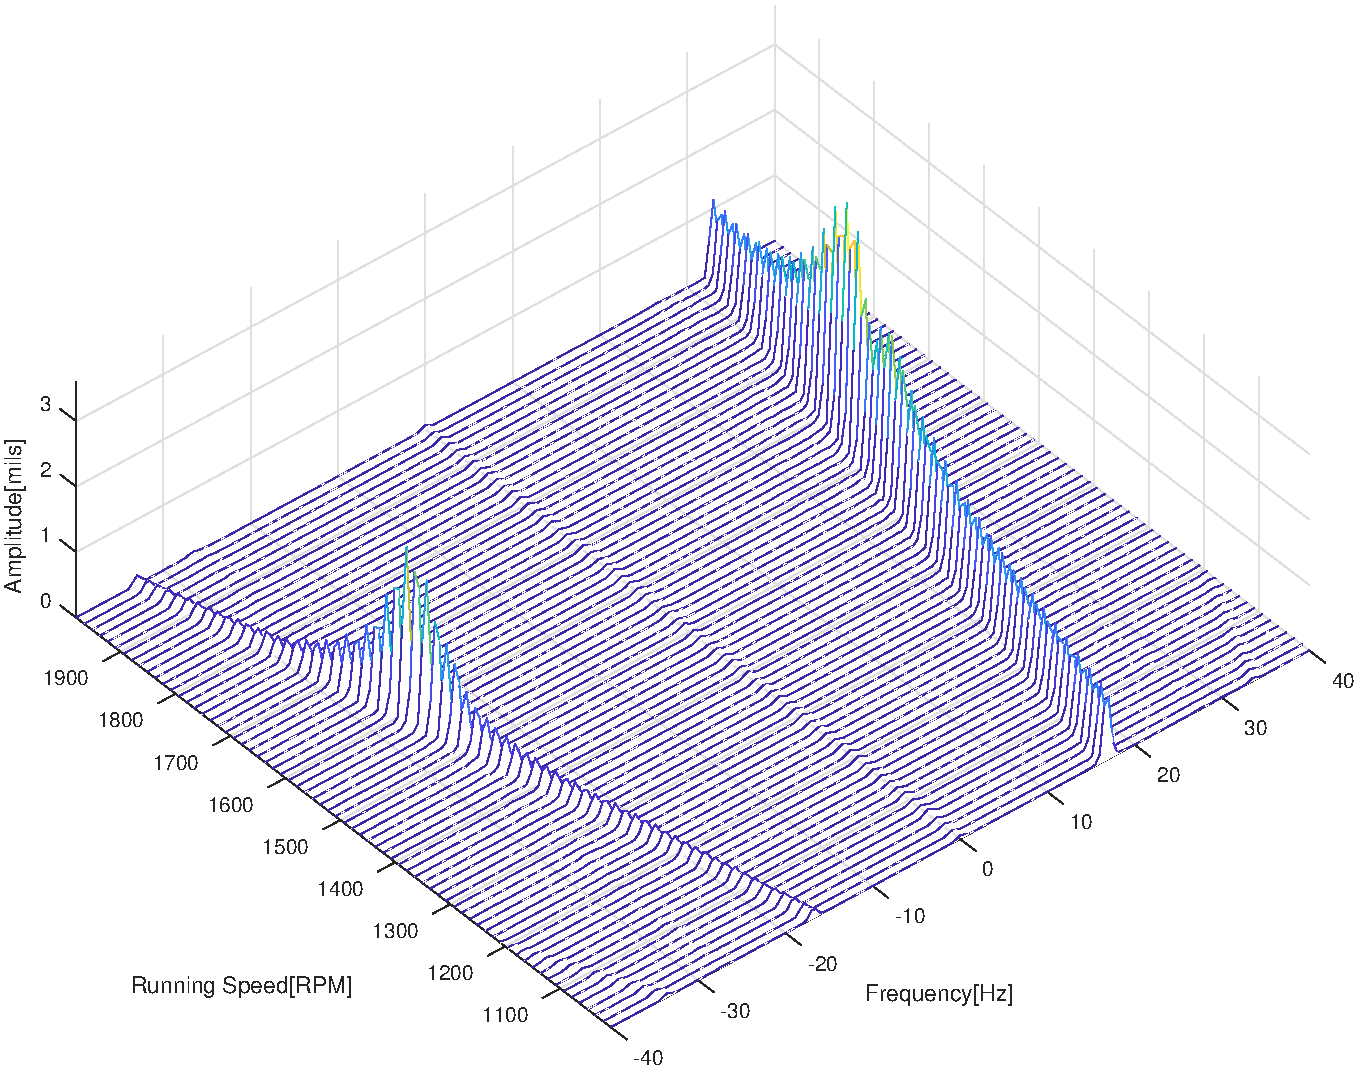
\includegraphics[width=.8\linewidth]{./figures/MagExampleCascade.pdf}
	\caption{Cascade of the experimental overhung rotor system.}
	\label{fig:MagExampleCascade}
\end{figure}
\begin{figure}[!htb]
	\def\width{.7\linewidth}
	\def\height{.4\linewidth}
	\def\sep{3em}
	\pgfplotsset{every picture/.style={trim axis left, trim axis right}, every axis/.style={ylabel style={xshift=0},xlabel style={yshift=0}}}%, every axis/.style={hide axis}}%
	\centering
	\import{}{./figures/MagExampleBode.tex}
	\caption{Bode diagram of the experimental overhung rotor filtered to 1X.}
	\label{fig:MagExampleBode}
\end{figure}
\section{Theoretical Model}
To create a finite element model for this rotor system the shaft will be discretized into 7 elements a disk at node 6 and bearings at nodes 1 and 4, as depicted in Figure \ref{fig:OverhungDiagram}. In the experiment, a small length of shaft continued after the overhung disk and has been included in this model. The AMB will be included as a nodal point element with with stiffness and damping to be derived in \S\ref{Active Magnetic Bearing}. Parameter values for the finite element model are provided in Table \ref{tab:OverhungParameters}. Discovered values such as $ \eta_v $ and the stiffnesses of bearing are listed here, but the process for their determination is discussed.
\begin{table}
	\caption{Properties of disks, shaft elements, and bearings of the theoretical model.} \label{tab:MagTheoryRotorTable}
	\centering
	\label{tab:OverhungParameters}
	\begin{tabular}{rcccccc}
							&$\rho\left[\frac{kg}{m^3}\right]$	&$r[m]$					&$\nu$				&$E[Pa]$			&$ \eta_v[s] $	&$ \eta_h $	\\\hline
		\textbf{Shaft}		&$7850$					&$0.005$				&$0.3$				&$\num{210E9}$		&$ 0.0002 $		&$ 0 $		\\[-.2em]
							&$\rho\left[\frac{kg}{m^3}\right]$	&$r[m]$					&$l[m]$				&					&				&			\\\hline
		\textbf{Disks}		&$7850$					&$0.0375$				&$0.025$			&					&				&			\\[-.2em]
							&$k_y\left[\frac{N}{m}\right]$		&$k_z\left[\frac{N}{m}\right]$		&$c_y\left[\frac{Ns}{m}\right]$&$c_z\left[\frac{Ns}{m}\right]$&				&			\\\hline
		\textbf{Bearing A}	&$1.7\e{5}$				&$2.2\e{5}$				&$68$				&$88$				&				&			\\[-.5em]
		\textbf{Bearing B}	&$2.04\e{5}$			&$2.64\e{5}$			&$81.6$				&$105.6$			&				&			\\
	\end{tabular}
\end{table}
First the model is formed to match the experimental results. Known parameters, such as beam lengths, beam diameters, density of the material, and geometry of the disk and rotor are used to begin construction of the model. Then, guesses are made for the stiffnesses in the rotor bearings. The first natural frequency is calculated with the resulting model and its value compared to the experimentally found natural frequency from the bode diagram (fig.\ref{fig:MagExampleBode}). Stiffness are then adjusted to better match the natural frequency, and this is repeated until the natural frequency of the model matches the experiment. After this process, the stiffness was determined to be around $ 2\e{5} \left[\frac{N}{m}\right]$.\par
It is evident by inspection of the Bode diagram for the experimental system (fig.\ref{fig:MagExampleBode}), and the 3D orbit, that there is anisotropy in the system, leading to the dip in amplitude of one plane of vibration. It is also known from inspection of the frequency spectrum in the cascade of figure \ref{fig:MagExampleCascade} that in this speed range the orbit is in the opposite direction of the rotation--a phenomena only possible with anisotropy of the stiffness. Figures \ref{fig:HorVertStiffAniCompare}\&\ref{fig:PosNegStiffAniCompare} demonstrate this affect anisotropy has on both the real coordinates, as well as positive and negative whirl amplitudes. \par 
\begin{figure}
\begin{subfigure}{\textwidth/2}
	\centering
	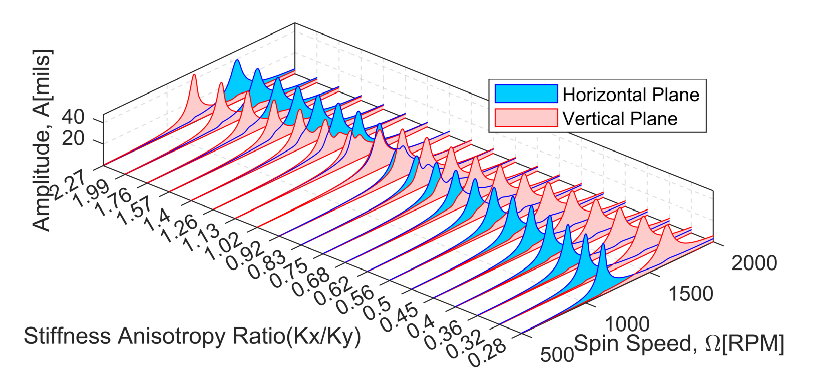
\includegraphics[width=\linewidth]{./figures/MagExampleHorVertStiffAniCompare.eps}
	\caption{3D Orbit of the experimental overhung rotor system.}
	\label{fig:HorVertStiffAniCompare}
\end{subfigure}
\begin{subfigure}{\textwidth/2}
	\centering
	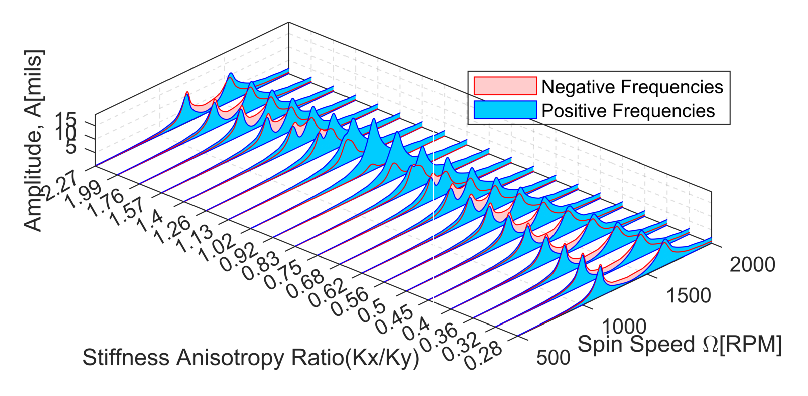
\includegraphics[width=\linewidth]{./figures/MagExamplePosNegStiffAniCompare.eps}
	\caption{3D Orbit of the experimental overhung rotor system.}
	\label{fig:PosNegStiffAniCompare}
\end{subfigure}
\end{figure}
Using the bode diagram, the stiffness anisotropy is adjusted until the shapes of the amplitudes and phases match the experimental results of figure \ref{fig:ExpExampleBode}. Then damping is added to the system to appropriately match the experimental results. The resulting bode diagram is Figure \ref{fig:MagTheoryBode}. Stiffnesses were determined to be $ k_y=1.7\e{5}[N/m]\ \&\ k_z=2.2\e{5}[N/m] $.
\begin{figure}[!htb]
	\def\width{.6\linewidth}
	\def\height{.4\linewidth}
	\def\sep{3em}
	\pgfplotsset{every picture/.style={trim axis left, trim axis right}, every axis/.style={ylabel style={yshift=.5em},xlabel style={yshift=0}}}%, every axis/.style={hide axis}}%
	\centering
	\import{figures/}{MagTheoryBode.tex}
	\caption{Bode Diagram of overhung system without AMB.}
	\label{fig:MagTheoryBode}
\end{figure}
And now the resulting system is further described with an expanded speed range of $ 20000[RPM] $. The new Campbell diagram of Figure \ref{fig:MagTheoryCampbell}, the roots locus of Figure \ref{fig:MagTheoryRootLocus}. Additionally, the first three mode shapes are plotted for this theoretical model (Figures \ref{fig:MagTheoryShape1}, \ref{fig:MagTheoryShape2}, \& \ref{fig:MagTheoryShape3}). Note that the first mode is conical in shape, but the disk is far from an antinode at node 6 so it does not experience significant gyroscopic moments. This idea is supported by the campbell diagram, fig. \ref{fig:MagTheoryCampbell}, as the first mode natural frequency does not change significantly over the speed range. On the other hand, the second mode has its antinode atode 6 so the disk experience maximum gyroscopic moments and the second mode critical speed is much more dependent on speed.
\begin{figure}[!htb]
	\def\width{.6\linewidth}
	\def\height{.4\linewidth}
	\def\sep{3em}
	\pgfplotsset{every picture/.style={trim axis left, trim axis right}, every axis/.style={ylabel style={yshift=.5em},xlabel style={yshift=0}}}%, every axis/.style={hide axis}}%
	\centering
	\import{figures/}{MagTheoryCampbell.tex}
	\caption{Campbell Diagram of the overhung system without AMB.}
	\label{fig:MagTheoryCampbell}
\end{figure}
\begin{figure}[!htb]
	\def\width{.6\linewidth}
	\def\height{.4\linewidth}
	\def\sep{3em}
	\pgfplotsset{every picture/.style={trim axis left, trim axis right}, every axis/.style={ylabel style={yshift=.0},xlabel style={yshift=0}}}%, every axis/.style={hide axis}}%
	\centering
	\import{}{./figures/MagExampleRootsLocus.tex}
	\caption{Roots Locus of overhung system without AMB.}
	\label{fig:MagTheoryRootLocus}
\end{figure}
\begin{figure}
	\def\cs{.29}
	\pgfplotsset{every picture/.style={trim axis left, trim axis right}, every axis/.style={yticklabel style={xshift=0,yshift=0},minor tick num=2}, grid style={line width=.1pt, draw=gray!20},major grid style={line width=.2pt,draw=gray!50},ticks=none,minor tick style={draw=none}}%, every axis/.style={hide axis}}% 
	\begin{subfigure}{\cs\textwidth}
		\centering
		\def\width{\linewidth}
		\def\height{\linewidth}
		\import{}{./figures/MagTheoryShape1.tex}
		\caption{Mode Shape 1.}
		\label{fig:MagTheoryShape1}
	\end{subfigure}
	\begin{subfigure}{\cs\textwidth}
		\centering
		\def\width{\linewidth}
		\def\height{\linewidth}
		\import{figures/}{MagTheoryShape2.tex}
		\caption{Mode Shape 2.}
		\label{fig:MagTheoryShape2}
	\end{subfigure}
	\begin{subfigure}{\cs\textwidth}
		\centering
		\def\width{\linewidth}
		\def\height{\linewidth}
		\import{figures/}{MagTheoryShape3.tex}
		\caption{Mode Shape 3.}
		\label{fig:MagTheoryShape3}
	\end{subfigure}
\end{figure}
\subsection{Active Magnetic Bearing}\label{Active Magnetic Bearing}
Magnetic pole-rotor relationship will be derived based on the detailed derivation in \cite{das2008vibration}. Assumptions made in this model are:
\begin{itemize}
	\item Air gap between the magnet pole face and the rotor is vanishingly small compared to the diameter of the shaft.\
	\item Flux leakage from the magnetic pole is negligible.
	\item Curvature of rotor surface under the pole face is ignored.
	\item A linear relationship of flux density and magnetic field is assumed.
	\item Hysteresis of the magnetic field is negligible.
\end{itemize}
These assumptions lead to a magnetic force due to coil current in the relationship of
\begin{equation}\label{key}
F_m=\frac{-k_mi^2}{l_g^2}
\end{equation}
where, $ k_m=\frac{\mu_0A_pN^2}{4} $, and $ \mu_0=4\pi\e{-7} $ is the absolute permeability in free air, $ N $ is the number of coil turns, $ A_p $ is the pole face area, $ i $ is the supplied electrical current, and $ l_g $ is the air gap.\par 
Consider a set of magnetic pole pairs in each the $ y\ \&\ z $ directions (i.e. One on the left and one on the right; one on top and one on bottom), where each pole pair has its own electrical circuit. There are 4 total magnets in this model, 2 in each direction, and 8 total poles where 2 form a magnet. All poles in the neutral position of the system will have a nominal air gap of $ g_0 $ and will be supplied by a bias current of $ i_0 $. Deviations of the current from this bias will be considered as $ i_y $ and $ i_z $. Deviations of the position from this neutral position are the displacements of the rotor at this beam axis location, $ v,\ \&\ w $. Therefore, total current will be $ (i_0\pm i_y)\ \&\ (i_0\pm i_z) $ for opposing poles in the $ y\ \&\ z $ directions respectively. Similarly, total gaps are given by $ (g_0\pm v)\ \&\ (g_0\pm w) $. Using these new definitions for the gap and current, and summing forces in the $ y\ \&\ z $ directions leads to the total forces
\begin{equation}\label{eq:MagneticForceNL}
F_y=K_m\left\{\left(\frac{i_0+i_y}{g_0+v}\right)^2-\left(\frac{i_0-i_y}{g_0-v}\right)^2\right\}\ \&\ F_z=K_m\left\{\left(\frac{i_0+i_z}{g_0+w}\right)^2-\left(\frac{i_0-i_z}{g_0-w}\right)^2\right\}
\end{equation}
where, $ K_m=k_m\cos(\alpha) $, and $ \alpha $ is half of the angle between the poles of a magnet. Linearizing the magnetic force equations \eqref{eq:MagneticForceNL}, while assuming the operating point for the system is where all positions and control currents are zero, results in
\begin{equation}\label{eq:MagneticForce}
F_y=k_ii_y+k_yv,\ \&\ F_z=k_ii_z+k_zw
\end{equation}
where, $ k_i=4K_m\frac{i_0}{g_0^2} $ is the current stiffness developed by the bias current, and $ k_y=k_z=k_s=-4K_m\frac{i_0^2}{g_0^3} $.
\subsubsection{Proportional Derivative Control}
A control algorithm is used to control the current sent to each pair of poles based on the position (proportional) and velocity (derivative) of the rotor. It is assumed that each set of pole pairs will receive opposite currents to act as a unit. Current control is given by 
\begin{equation}\label{eq:ControlCurrent}
i_y=-k_g(k_pv+k_v\dot{v}),\ \&\ i_z=-k_g(k_pw+k_v\dot{w})
\end{equation}
where, $ k_g $ is the power amplifier gain, $ k_p $ is the proportional gain, and $ k_v $ is the derivative gain. The total linearized force becomes
\begin{equation}\label{key}
F_y=-(k_gk_ik_p-k_s)v-k_gk_ik_v\dot{v},\ \&\ F_z=-(k_gk_ik_p-k_s)w-k_gk_ik_v\dot{w}
\end{equation}
so then the stiffness of the AMB is $ k_{mag}=(k_gk_ik_p-k_s) $ and the damping is $ d_{mag}=k_gk_ik_v $. As an equation of nodal stiffness and damping in the finite element system it can be represented by
\begin{equation}\label{eq:DiskNodeEquationofMotion}
\bunderline{\mathbf{D}}^m\dot{\vec{\mathbf{q}}}_k+\bunderline{\mathbf{K}}^m\vec{\mathbf{q}}_k=0
\end{equation}
where,
\begin{equation*}
\def\cs{2em}
\begin{array}{cc}
\bunderline{\mathbf{K}}^m=\left[\def\arraystretch{.8}\arraycolsep=0pt\begin{array}{cccccc}
\makebox[\cs]{$k_{mag}$}&\makebox[\cs]{0}&\makebox[\cs]{0}&\makebox[\cs]{0}&\makebox[\cs]{0}&\makebox[\cs]{0}\\
0&k_{mag}&0&0&0&0\\
0&0&0&0&0&0\\
0&0&0&0&0&0\\
0&0&0&0&0&0\\
0&0&0&0&0&0
\end{array}\right] & \bunderline{\mathbf{D}}^m=\left[\def\arraystretch{.8}\arraycolsep=0pt\begin{array}{cccccc}
\makebox[\cs]{$d_{mag}$}&\makebox[\cs]{0}&\makebox[\cs]{0}&\makebox[\cs]{0}&\makebox[\cs]{0}&\makebox[\cs]{0}\\
0&d_{mag}&0&0&0&0\\
0&0&0&0&0&0\\
0&0&0&0&0&0\\
0&0&0&0&0&0\\
0&0&0&0&0&0
\end{array}\right]
\end{array}
\end{equation*}
Knowing that the amplitude of vibration, $ A $, in the experimental system peaks at about 10 mils, or $ 2.54\e{-4}[m] $, the greatest possible velocity for synchronous vibration is determined using the simple equation $ v=(A/2)\omega $, where $ \omega $ is the whirl speed in rad/s. Under the assumption of synchronous vibration, $ \omega $ during the natural frequency is then $ 167.6[Rad/s] $. Leading to a velocity, $ v $, of $ 0.02[m/s] $. Looking also at the velocity in the upper speed range, knowing that the amplitude of vibration after the first natural frequency is equal to the eccentricity of the unbalance. With an eccentricity of $ 1\e{-5} $ and an upper speed of $ 15000[RPM] $, the velocity is calulated to be $ 0.008[m/s] $. Since the estimated velocity during the natural frequency is higher, it will be used to limit the output of the AMB controller. Since the total voltage supply of most digital to analog converters is limited to $ 10[V] $ the control voltage is calculated to be within this range for the given velocity and positions that will be seen under synchronous vibration. This results in a limitation of the term $ k_v $, which is proportional to the voltage control signal that is sent to the amplifier for conversion to control current. A value of $ 480[Vs/m] $ would max the converter, so the value to be determined must be less than this. With a similar, but separate, evaluation of the displacement leads to a cap of $ 500000[V/m] $ for $ k_p $--a value not anticipated to be necessary. The maximum force due to unbalance is $ \epsilon m_d\Omega^2 $, where $ \epsilon $ is the eccentricity, and $ m_d $ is the mass of the disk. At the maximum speed expected of $ 15000[RPM] $, the force will be $ 24[N] $. To counteract this force with a single coil would require $ 1.25[A] $, or $ 0.625[A] $ per coil in a opposing pair. The amplifier gain is assumed to be programmable to $ k_g=1[A/V] $, this leads to a reasonable choice of bias current at $ 0.5[A] $ to maintain a good resolution on the voltage output of the controller. The voltage should not need to peak above $ 1.25[V] $, and will rest at an output of $ 0.5[V] $. Now in the next section, control parameters $ k_v\ \&\ k_p $ will be determined to maximize stability of the system while also minimizing vibration.
\section{Addition of Magnetic Bearing to the Rotor Model}
In order to measure the effectiveness of the AMB, the Stability of the theoretical model before the addition is shown in Figure \ref{fig:MagTheoryStability}. The magnetic bearing added is modeled after a magnetic bearing that is currently in the lab at California Polytechnic State University. This theoretical exercise is intended to be followed by experimental verification not included in this work. The parameters used are listed in \ref{tab:MagBearingParameters} as well as the control values whose determinations will be evaluated.\par 
First the position of the AMB must be determined. By inspection of the mode shapes, it is evident that in the first mode (the mode we are most concerned about suppressing) a conical mode shape exists with increasing amplitude toward the end of the beam after the second bearing. It is also known that the source of vibration, the rotating disk, is located at nodal index 6. With both these pieces of information, node 7 is chosen as a starting point for the AMB for two reasons: having the AMB closer to the source of vibration reduces the phase lag between the source and the bearing, increasing the effectiveness of control; amplitude of vibration, according to the mode shape, is higher on the outboard side of the disk and placing the AMB on this side will minimize more vibration.\par 
 To determine best derivative control, the proportional control was set to zero and the derivative increased until the first mode on the Roots locus(fig. \ref{fig:MagTheoryRootLocus}) moved away from the imaginary axis, becoming more damped. The resulting movement of the Roots on the Roots Locus is given in Figure \ref{fig:MagTheoryRootLocusControllerTune}. Notice how none of the new modes that appear on the roots locus cross the real plane--this demonstrates the stability of the new system. Stability of the system with the AMB addition is confirmed in the stability plot of Figure \ref{fig:MagTheoryStabilityWith}. In fact from the roots locus with $ k_v=1 $ to the roots locus with $ k_v=10 $ the first mode of vibration is completely relegated to the imaginary axis and not reaching break-away for this entire speed range--this indicates that the first mode has been over-damped.\par 
 Proportional control, $ k_p $, was added after the ideal derivative control was determined, but it did not improve the performance of the controller. It is possible that the stiffness of the bearing inherent to the bias current is sufficient. In any case, proportional control in this scenario is only adding stiffness to the system, and with the objective being to minimize vibration, $ k_p $ does not help. So the optimal control is determined to be with $ k_v=10[Vs/m] $. The remaining parameters for this resulting controller are listed in table \ref{tab:MagBearingParameters}. It is worthwhile to note that this optimal control is standing on the basis that the feedback is of synchronous vibration only. In a scenario where there is significant sub or super-synchronous vibrations, this controller may exceed its voltage limit. It is recommended that the feedback signal be filtered to match rotor speed to ensure this scenario does not take place. Furthermore, without at least low-pass filtering of the feedback signal the control would certainly provide out of range signals due to the volatile nature of derivatives of discrete signals.\par 
 The frequency spectrum is provided showing the result of the AMB application in the bode diagram of Figure \ref{fig:MagTheoryBodeCompare}. Certainly it can be concluded that the AMB is successfully performing the desired task of reducing the vibration while also inproving the stability of the system.\par 
 Now the result from this synthesis exercise can be implemented on the actual experimental test rig with the AMB set to the control parameters suggested. The power of the finite element method in this application is the ability to move components around with ease. For instance, with the changing of just two parmeters in the input file for this model, a new simulation is create for complete levitation of the overhung rotor. The AMB is put in place of bearing b and the resulting frequency spectrum is plotted in Figure \ref{fig:MagLevTheoryBodeCompare}
\begin{table}
	\centering
	\caption{Active Magnetic Bearing Parameters.}
	\begin{tabular}{cccccccc}
		$\alpha[rad]$&$g_0[m]$&$i_0[A]$&$k_p[\frac{V}{m}]$&$k_v[\frac{Vs}{m}]$&$k_g[\frac{A}{V}]$&$ N[\#]$&$A_p[m^2]$\\\hline
		$\frac{\pi}{8}$&$2.5\e{-3}$&$0.5$&$0$&$10$&$1$&$800$&$\frac{5}{100*100}$
	\end{tabular}
	\label{tab:MagBearingParameters}
\end{table}
\begin{figure}
	\begin{subfigure}{\textwidth/2}
		\def\width{.8\linewidth}
		\def\height{.4\linewidth}
		\pgfplotsset{every picture/.style={trim axis left, trim axis right}, every axis/.style={ylabel style={yshift=-20},xlabel style={yshift=35}},every x tick scale label/.style={at={(xticklabel* cs:1,.3cm)},anchor=near xticklabel}}%, every axis/.style={hide axis}}%
		\centering
		\import{figures/}{MagTheoryStability.tex}
		\caption{Stability plot of rotor without AMB, threshold of stability:$ \ 4646[RPM] $.}
		\label{fig:MagTheoryStability}
	\end{subfigure}
	\begin{subfigure}{\textwidth/2}
		\def\width{.8\linewidth}
		\def\height{.35\linewidth}
		\pgfplotsset{every picture/.style={trim axis left, trim axis right}, every axis/.style={xlabel style={yshift=-2em},xlabel style={yshift=25,at={(axis description cs:0.5,1.05)},anchor=north}},every x tick scale label/.style={at={(xticklabel* cs:1,.3cm)},anchor=near xticklabel}}%, every axis/.style={hide axis}}%
		\centering
		\import{figures/}{MagTheoryStabilityWith.tex}
		\caption{Stability plot of rotor with AMB, indicates complete stability through speed range.}
		\label{fig:MagTheoryStabilityWith}
	\end{subfigure}
\end{figure}
\begin{figure}[!htb]
	\def\width{.7\linewidth}
	\def\height{.5\linewidth}
	\def\sep{3em}
	%\pgfplotsset{every picture/.style={trim axis left, trim axis right}}%, every axis/.style={ylabel style={yshift=0em},xlabel style={yshift=0}}}%, every axis/.style={hide axis}}%
	\centering
	\import{figures/}{MagTheoryRootLocusControllerTune.tex}
	\caption{Roots locus of Overhung rotor system with varying $ k_v $.}
	\label{fig:MagTheoryRootLocusControllerTune}
\end{figure}
\begin{figure}[!htb]
	\def\width{.6\linewidth}
	\def\height{.4\linewidth}
	\def\sep{3em}
	\pgfplotsset{every picture/.style={trim axis left, trim axis right}}%, every axis/.style={ylabel style={yshift=0em},xlabel style={yshift=0}}}%, every axis/.style={hide axis}}%
	\centering
	\import{figures/}{MagTheoryBodeCompare.tex}
	\caption{Bode diagram at node 6 comparing the rotor without AMB(solid) and with AMB(dashed).}
	\label{fig:MagTheoryBodeCompare}
\end{figure}
\begin{figure}[!htb]
	\def\width{.6\linewidth}
	\def\height{.4\linewidth}
	\def\sep{3em}
	\pgfplotsset{every picture/.style={trim axis left, trim axis right}}%, every axis/.style={ylabel style={yshift=0em},xlabel style={yshift=0}}}%, every axis/.style={hide axis}}%
	\centering
	\import{figures/}{MagLevTheoryBodeCompare.tex}
	\caption{Bode diagram at node 6 comparing the rotor without AMB(solid) and with AMB(dashed) for complete levitation at node 4.}
	\label{fig:MagLevTheoryBodeCompare}
\end{figure}
%\chapter{Overhung}
	\section{Introduction}
		Overhung rotors are widely used in industrial turbo-machines. For certain gas turbines, gyroscopic effects of the disks may almost double the critical speeds of the rotor systems, compared to normal mechanical vibration systems. In addition, the asymmetry of the bearing stiffness will bring more complication to a rotor system. Even though there are many established publications about how to theoretically model an overhung rotor with anisotropic bearings (\cite{Genta}-\cite{Ishida},\cite{Dimarogonas}), very few papers compared the theoretical models with experimental results. Ishida al etc.\cite{Ishida} derived a sophisticated mathematical model to theoretically investigate the nonstationary vibration of a flexible rotor with nonlinear spring parameters during acceleration. They employed an asymptotic method to compute the first approximate solution to vibration response. Then, they calculated the amplitude variation curves of each oscillation component using complex-FFT. Furthermore, they inspected how each nonlinear component in polar format affected dynamic vibration. They proposed a unique signal processing method called complex-FFT where the rotor whirling plane is coincident with the complex plane. The whirling direction of the rotor can be judged by filtering the vibration signals at different frequencies using complex-FFT method. However, the complex-FFT doesn’t provide instrumentation phase angle information and full spectrum cascaded plots.
		\par
		Gunter etc. (\cite{Gunter}, \cite{Gunter 93}) performed investigations about the forward and backward modes of overhung rotors through theoretical models and Finite Element Analysis. Like the majority of the publications, they use FFT to analyze their simulation results. In 1993, Southwick, Goldman, and Muszynska (\cite{Goldman}-\cite{Southwick 94}) introduced the new powerful “full spectrum” plot in rotating machinery vibration and rotor dynamics. Since then, Bently Nevada Corporation has installed full spectrum cascade plots in all of their major machinery data acquisition software package entitled as ADRE system. Compared to “traditional (half) spectrum” FFT plot, full spectrum can extract more significant diagnostic information from the original signals generated by X, Y transducers, this allows engineers to determine whether the vibration response is forward or backward with respect to rotational direction of the shaft. As a powerful tool for interpreting the vibration signals of rotating machinery, the full spectrum plots display the correlation between the vibration signals from the X and Y transducers. Based on reference (\cite{Bently}-\cite{Southwick 94}), Bently Nevada of GE Energy builds a multi-channel signal processing and data acquisition system, the ADRE Sxp Software and the 408 DSPi (Dynamic Signal Processing Instrument) respectively. Unlike any other data acquisition systems, ADRE 408 SDPi is an extremely versatile system designed for real-time highly parallel signal processing and presentation. Cascade full spectrum plots are embedded into all ADRE software which are installed on the majority of turbo-machines in industry.
		\par
		Muszynska (1996) \cite{Muszynska 96} methodically investigated the dynamic behaviors of a vertically configured overhung imbalanced rotor supported by flexible anisotropic bearings by theory and experiments. She concluded that the interaction of imbalance and shaft bow causes the synchronous forced precession of the rotor to be forward or backward. Furthermore, she investigated the situation in which the mid-span rotor sections precess one way, while the outboard disk precesses the other. The phenomenon is partly attributed to the relationship between the unbalances in terms of their relative direction. Ishida et al. (2008) \cite{Ishida 2008} theoretically investigated internal resonances near both the primary and the gravity critical speeds for a rotor system of an asymmetric shaft supported at both ends and a disk installed in the middle; nonlinearities of the system induced by bearing clearances were thoroughly explored. Nagasaka et al. (2008) \cite{Nagasaka} did further research by studying internal resonance between the forward and backward whirl modes near both the primary and the secondary critical speeds for a simply-supported rotor system with  asymmetric shaft. Based on above research, Nandakumar et al. (2010) \cite{Nandakumar} extended their research to an overhung rotor with substantial gyroscopic effects and relatively large lateral vibration using the method of multiple scales (MMS). The authors derived the theoretical nonlinear equations of motion for an asymmetrical overhung rotor running near its gravity critical speed. The authors examined how gyroscopic effects contribute on maximum resonant amplitudes, which disclose some interesting phenomena induced solely by nonlinearities of the system.
		\par 
		Yim et al. (2012) \cite{Yim} studied the dynamic response of a flexible shaft with a disk subjected to axial forces for two overhung rotor systems using transfer matrix method. They concluded that, under the force load, the gyroscopic effect not only increases the critical axial force, but also changes the instability type from divergence to flutter. Ma et al. (2015) \cite{Ma}experimentally investigated the vibration response of an overhung rotor under sudden unbalance excitation due to the blade loss and quantitatively assessed the impact effect. The effect of the sudden unbalance is tested in both the subcritical state and the supercritical state. The results demonstrate that the response of the system to sudden imbalance contains frequencies from the impact response as well as frequencies due to rotational speed. A flexible rotor was shown to excite more from sudden imbalance than a more rigid rotor. Ma et al. (2015) \cite{Ma, H} presents a finite element model of the oil film instability of an overhung rotor with both parallel and angular misalignments including the gyroscopic effect. Oil film bearings are simulated using a non-linear oil-film force model, assuming short-length bearings. The validity of the model is verified by comparison to experimental results in published literature. Results show that misalignment of the coupling can delay the first mode of vibration and even reduce its amplitude.
		\par 
		Unfortunately, to the best of the authors’ knowledge, there are no publications about how to actually generate the cascade full spectrums directly from either X, Y transducers or simulation results. If we successfully solve this problem, we can predict what will happen in experiments from theoretical models. In this research, we will solve the following 4 problems. 1. We construct 3D full spectrum cascade plots using complex FFT through MATLAB programing. 2. We use tracking windows to filter the transducer data to nX components of rotor speed when the rotor starts up or runs down. 3. We experimentally compare our results with ADRE data. The results are directly comparable and the MATLAB plots, using our method, provide opportunity of further post processing full spectrum data. 4. Theoretical results of overhung rotor are converted into 3D full spectrum plots which will be compared with experimental data. The results presented in this paper match with experiments with confidence. More importantly, effects of different components of the theory are able to be determined. This allows for better diagnoses of real rotor systems. Stiffness of the bearings is determined by comparing theoretical natural frequencies to natural frequencies determined by experimentation. Using a Bode plot for each $xz$ and $yz$ plane, Figure \ref{fig:Figure_14}, the natural frequency of the experimental apparatus is determined for each plane. The equations of motion \ref{math:1}, with disregard for forcing and moment equations on the right hand side, are coupled with the total stiffness matrix \ref{math:10} to provide a system of equations that is dependent only on time, speed and the unknown bearing stiffness parameters. This system of equations is used to solve for the natural frequencies in terms of the speed and the bearing stiffness using the eigenvalue problem. Different values of bearing stiffness are chosen in each plane and a Campbell diagram is used to solve for the natural frequency as a function of speed. Values of stiffness are iterated until the theoretical and experimental natural frequencies match.\par
		Skew angle is determined by comparing theoretical and experimental angular displacement vibrations. Deducing the angular displacement from experiment is not easy to do, as transducers are observing the vibration of the shaft and not the angle of the disk. A method for determining the angle was employed in which displacements from two sets of transducers is compared. \par
		To the best of the authors’ knowledge, there are no papers which provide direct comparison between theoretical models and experimental results using full spectrum analysis. Experimental work sometimes uses full spectrum but most often it uses half spectrum. Analytical work that reports full spectrum does not correlate phase angel to instrument measurement.
		\par
	\section{Theoretical Model}
		The theoretical model used to simulate the experimental apparatus is depicted in Figures \ref{fig:Figure_1} and \ref{fig:Figure_2}. Equations of motion \ref{math:1} are determined using conservation of momentum and a dynamic analysis of the disk mass and inertial changes. The forcing functions on the right hand side of \ref{math:1} include forces due to acceleration of the shaft so that the simulation can include change in speed of the shaft and gyroscopic effects, such as a start-up or run-down. Moment equations are presented as pertaining to the change in angular momentum of the disk (\cite{Genta}, \cite{Muszynska},\cite{Gunter 93}).\par
		\begin{equation}
			\centering
			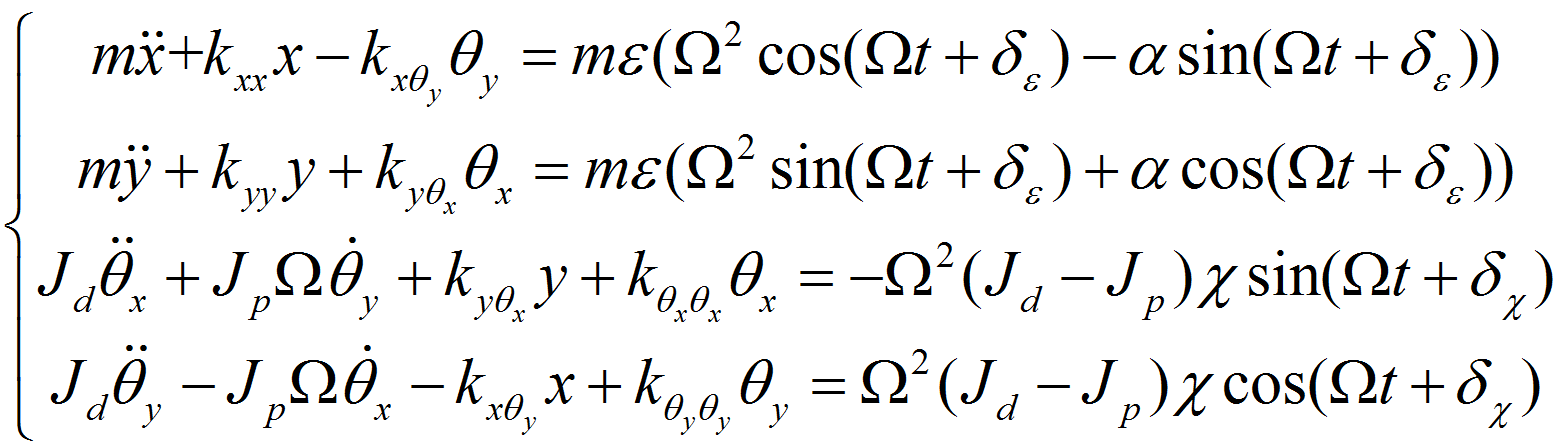
\includegraphics[scale=0.25]{./figures/Images/Math_1}
			\label{math:1}
			\centering
		\end{equation}
		\begin{figure}[h]
			
			\begin{subfigure}[b]{.5\textwidth}
 				\centering
 				 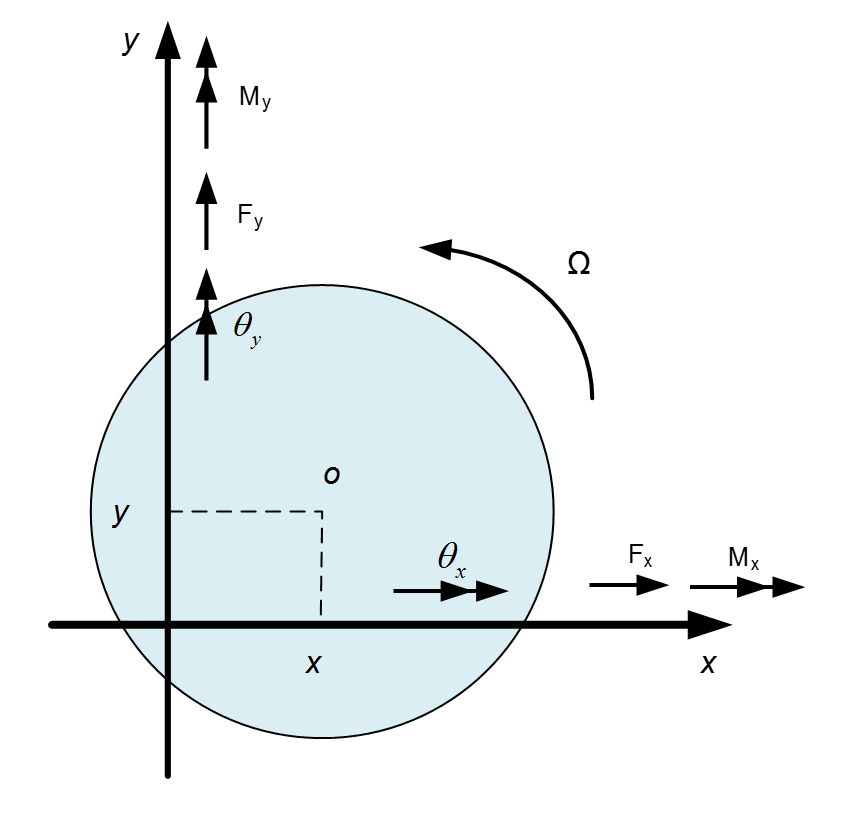
\includegraphics[width=.75\linewidth]{./figures/Images/Figure_1a}
 				 \caption{Displacements, rotations, forces and moments}
 				 \label{fig:Figure_1a}
 				 \centering
			\end{subfigure}%
			\begin{subfigure}[b]{.5\textwidth}
  				\centering
  				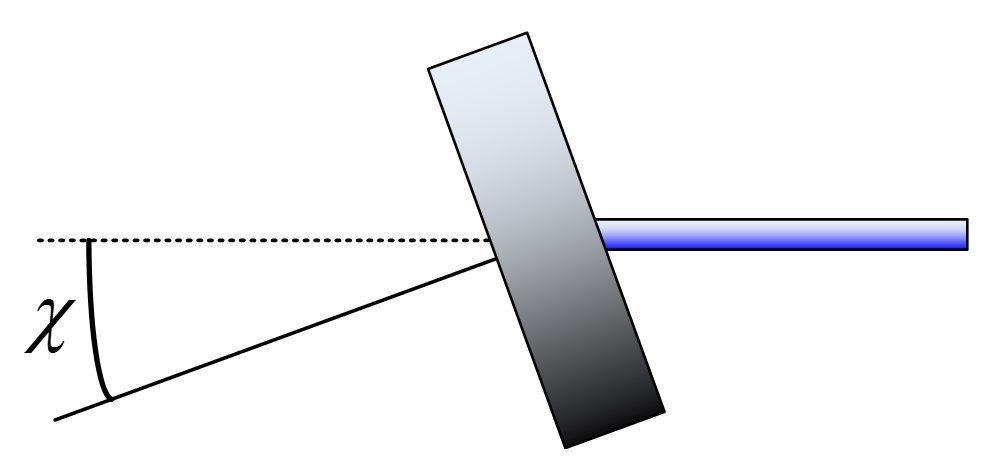
\includegraphics[width=.75\linewidth]{./figures/Images/Figure_1b}
  				\caption{Depiction of skew angle $\chi$}
  				\label{fig:Figure_1b}
  				\centering
			\end{subfigure}
			\caption{Experimental apparatus mathematical representation}
			\label{fig:Figure_1}
			
		\end{figure}
		\begin{figure}[h]
			\centering
			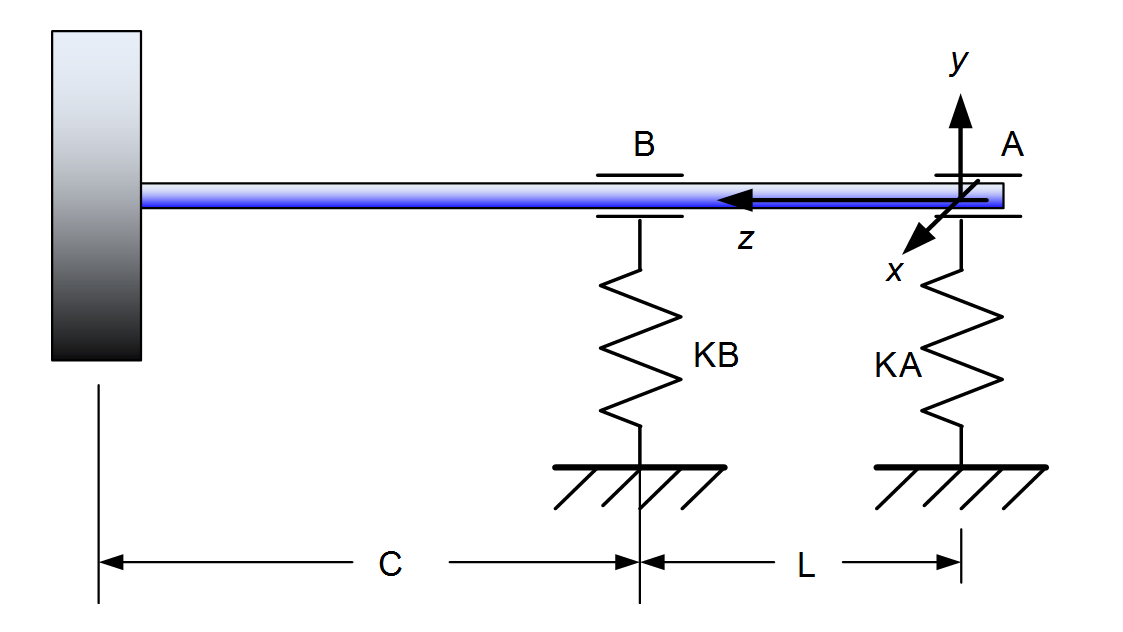
\includegraphics[scale=.25]{./figures/Images/Figure_2}
			\caption{Diagram showing important parameters}
			\label{fig:Figure_2}
			\centering
		\end{figure}
		The total stiffness constants of the system are determined from geometry and properties of the rotor bearings, and divided into two main contributions from the bending of the shaft and the suspension of the bearings. These two contributions are considered independent to solve for each contribution and then are combined in series to determine the total stiffness.\par
		Case (A) Flexible shaft with rigid bearings. Flexible Influence coefficients method in the general form of \ref{math:2} is used to derive flexibility matrix  which can be applied in both $xz$ and $yz$ plane, respectively. Since the shaft is considered to be isotropic, the matrix is identical for the xz and the $yz$ plane (\cite{Ishida},\cite{Dimarogonas}).\par
		\begin{equation}
			\centering
			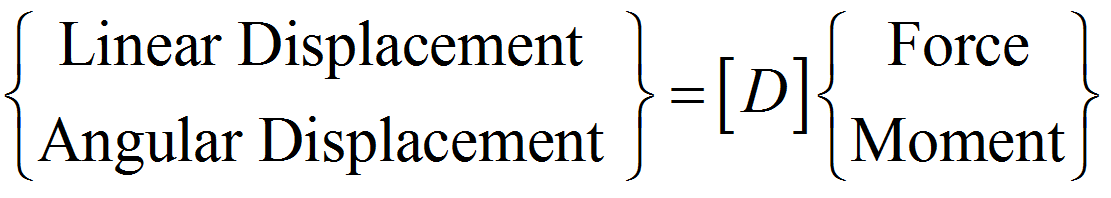
\includegraphics[scale=.25]{./figures/Images/Math_2}
			\label{math:2}
			\centering
		\end{equation}
		\begin{equation}
			\centering
			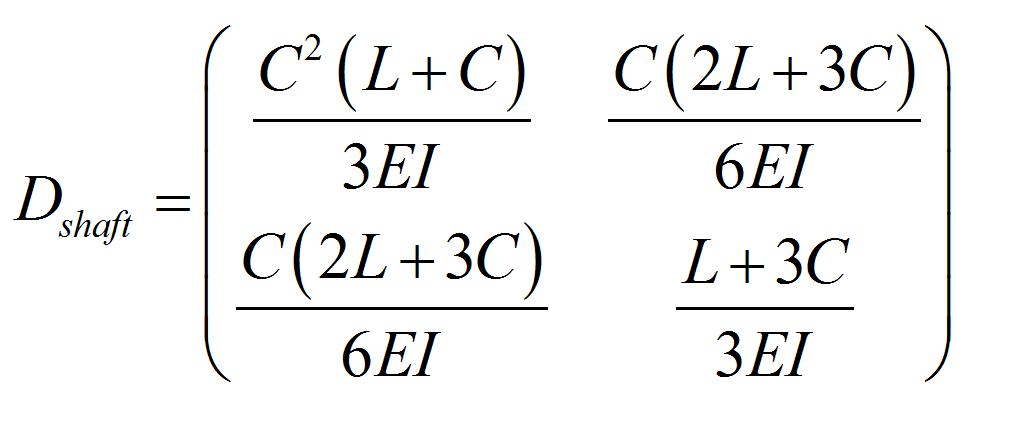
\includegraphics[scale=.25]{./figures/Images/Math_3}
			\label{math:3}
			\centering
		\end{equation}
		Case (B) Rigid shaft with flexible bearing. The stiffness matrix is derived in the general form of \ref{math:4} using stiffness influence coefficients method.\par
		\begin{equation}
			\centering
			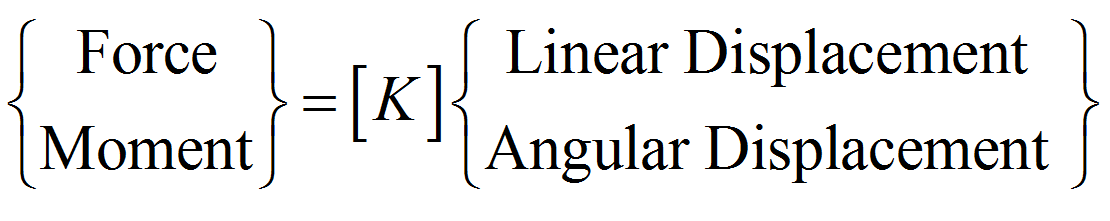
\includegraphics[scale=.25]{./figures/Images/Math_4}
			\label{math:4}
			\centering
		\end{equation}
		\begin{equation}
			\centering
			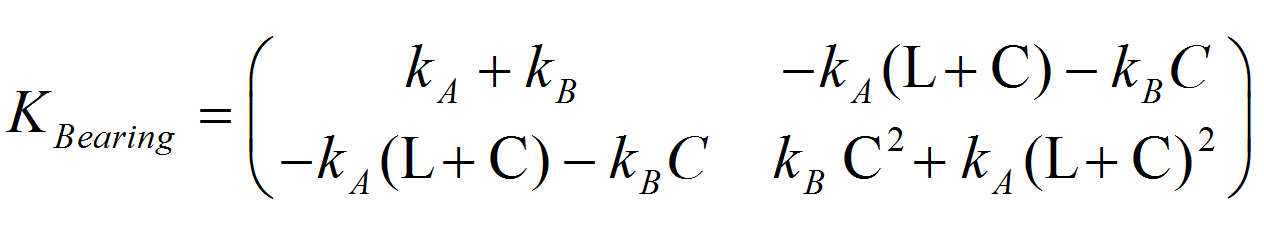
\includegraphics[scale=.25]{./figures/Images/Math_5}
			\label{math:5}
			\centering
		\end{equation}
		In order to combine the bearing stiffness with the shaft stiffness, both are added as flexibility matrices.\par
		\begin{equation}
			\centering
			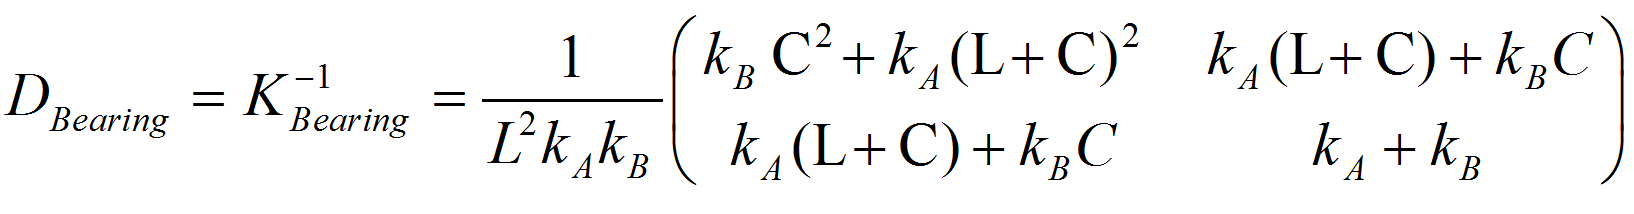
\includegraphics[scale=.25]{./figures/Images/Math_6}
			\label{math:6}
			\centering
		\end{equation}
		Apply to $xz$ and $yz$ plane, respectively to account for anisotropy of bearing stiffness for different planes.\par
		\begin{equation}
			\centering
			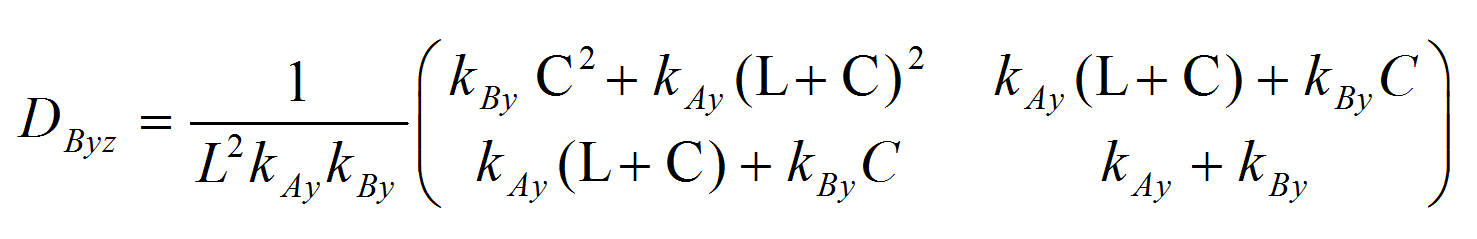
\includegraphics[scale=.25]{./figures/Images/Math_7}
			\label{math:7}
			\centering
		\end{equation}
		\begin{equation}
			\centering
			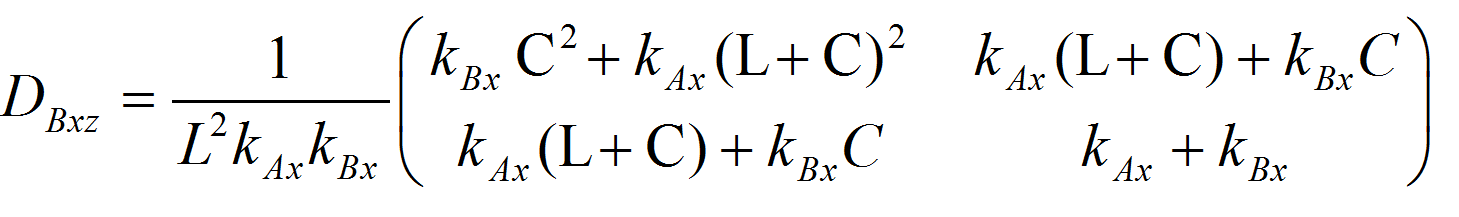
\includegraphics[scale=.25]{./figures/Images/Math_8}
			\label{math:8}
			\centering
		\end{equation}
		Total flexibility matrices in $xz$ and $yz$ plane are:\par
		\begin{equation}
			\centering
			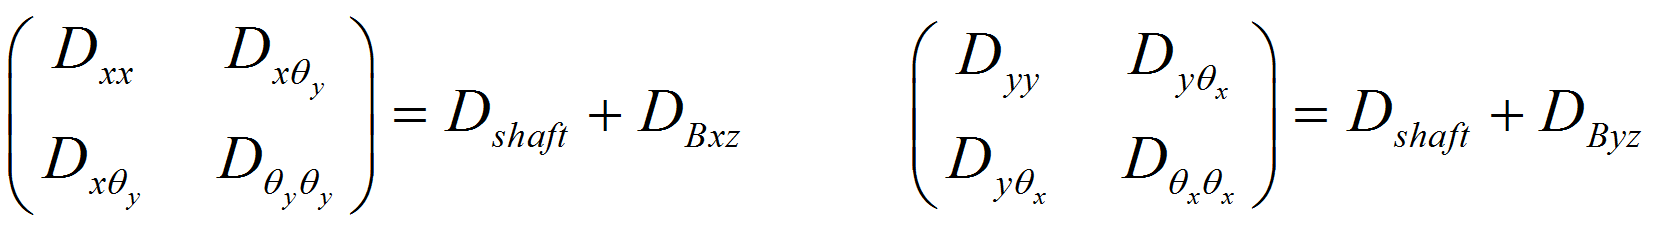
\includegraphics[scale=.25]{./figures/Images/Math_9}
			\label{math:9}
			\centering
		\end{equation}
		Total stiffness matrices are shown in \ref{math:10}, which are applied in equations of motion \ref{math:1}.\par
		\begin{equation}
			\centering
			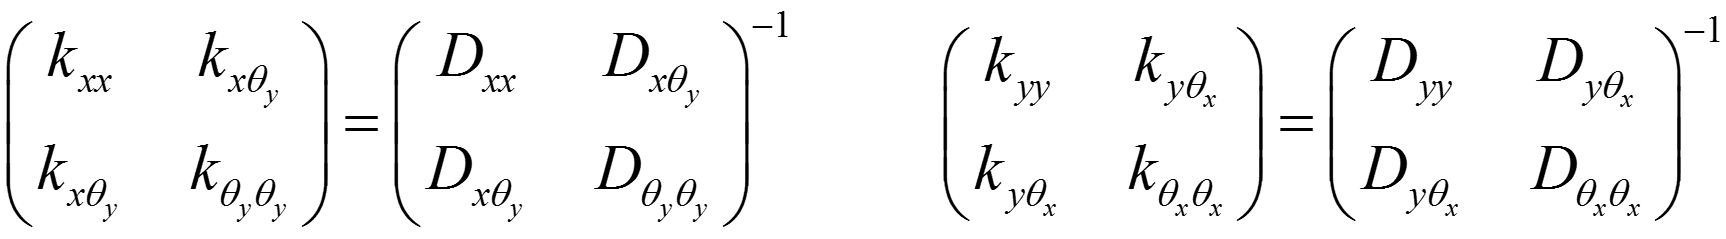
\includegraphics[scale=.25]{./figures/Images/Math_10}
			\label{math:10}
			\centering
		\end{equation}
			
	\section{Experimental apparatus}
		Our experimental apparatus consists of the GE (Formally Bently Nevada) RK4 rotor kit, the ADRE 408 Dspi Data asset condition monitoring equipment, and a laptop with the ADRE sxp software (Figure \ref{fig:Figure_3}). Four eddy current displacement transducers are used to measure the vibration of the shaft. The ADRE 408, when coupled with ADRE sxp, is capable of providing real-time signal processing from the rotor system in meaningful figures.\par
		\begin{figure}[H]
			\begin{subfigure}[b]{.5\textwidth}
				\centering
				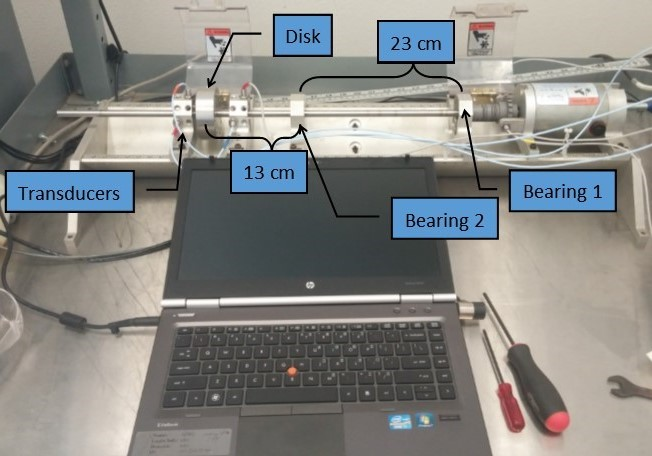
\includegraphics[width=.95\linewidth]{./figures/Images/Figure_3.jpg}
				\caption{Schematic of rotor geometry}
				\label{fig:Figure_3a}
				\centering
			\end{subfigure} %
			\begin{subfigure}[b]{.5\textwidth}
				\centering
				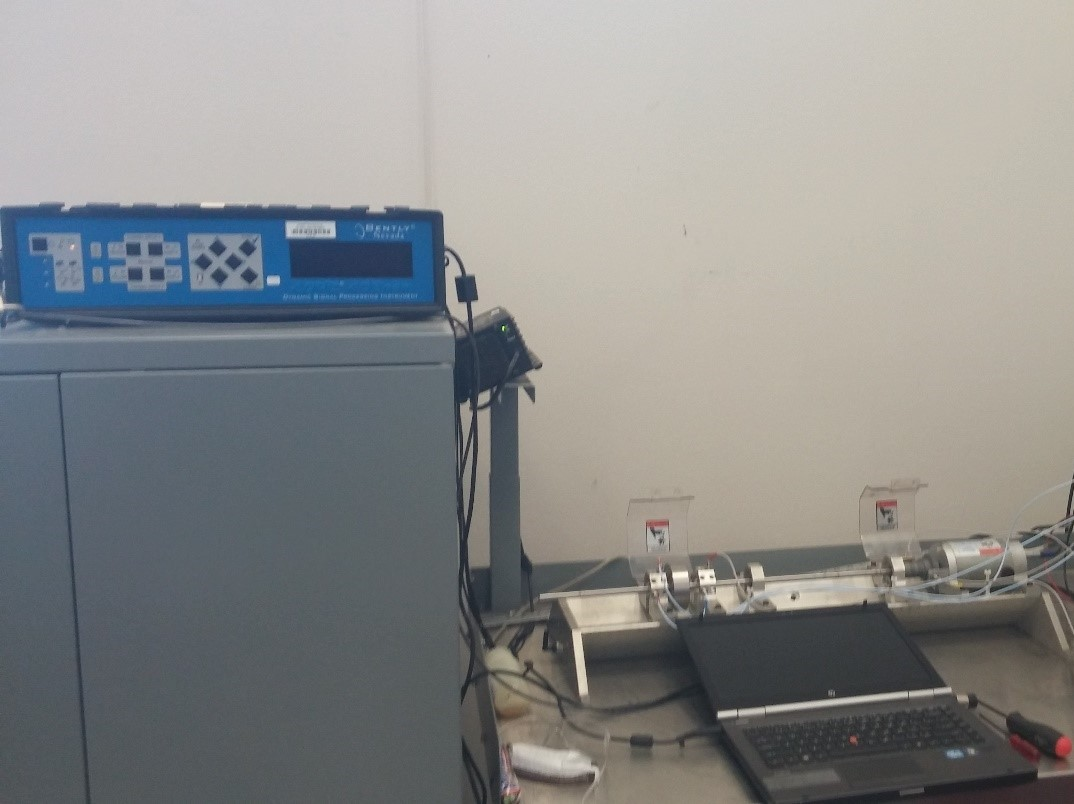
\includegraphics[width=.95\linewidth]{./figures/Images/Figure_3b.jpg}
				\caption{Overview of apparatus}
				\label{fig:Figure_3b}
				\centering
			\end{subfigure}
			\caption{Experimental apparatus}
			\label{fig:Figure_3}
		\end{figure}
		\begin{table}[H]
			\centering
			\caption{Rotor parameters}
			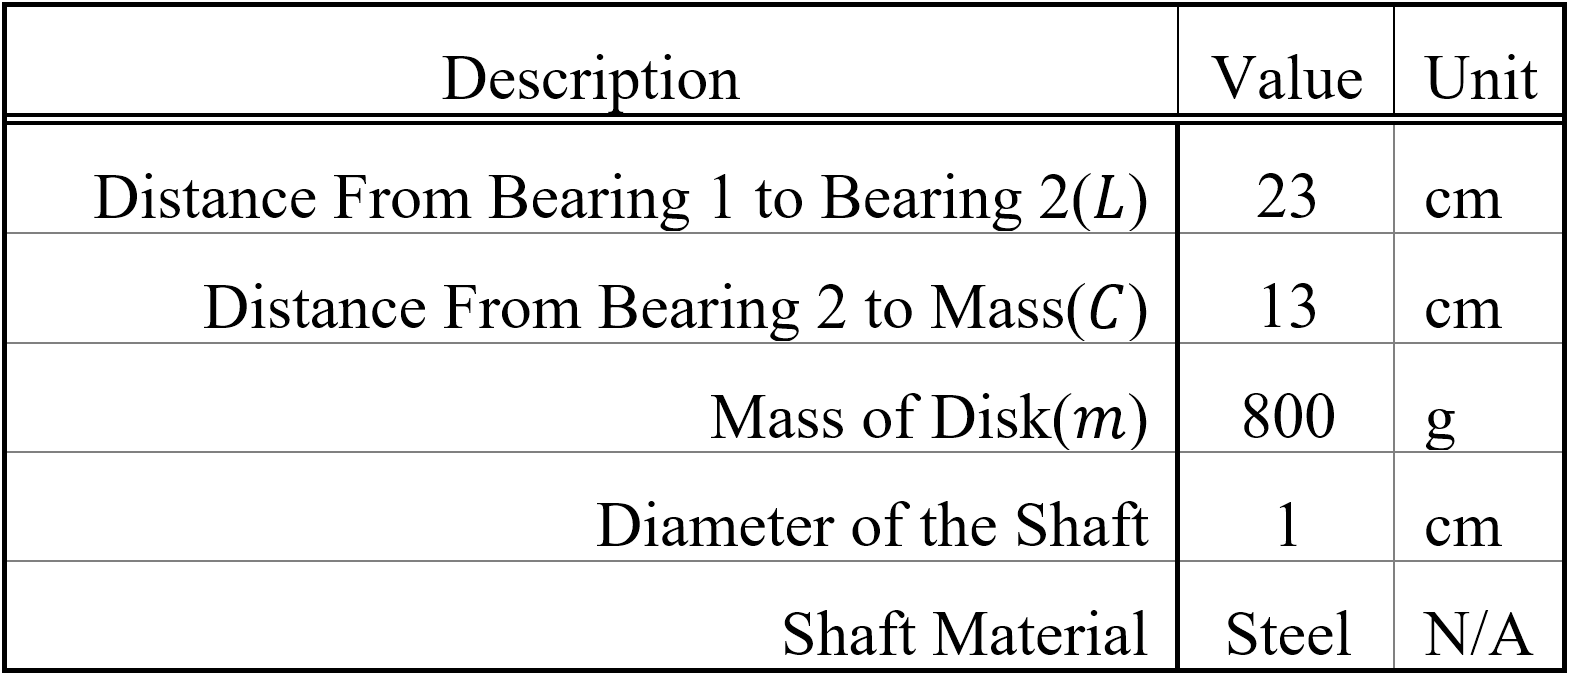
\includegraphics[scale=.25]{./figures/Images/Table_1}
			\label{tab:Table_1}
			\centering
		\end{table}
	\section{Identify the bearing stiffness parameters from experimental data}
		With the experimental data we were able to identify the natural frequency in the horizontal and vertical directions from the Bode plot of each horizontal and vertical transducer. From the theoretical equations of motion, the eigenvalue problem can be used to solve for the natural frequencies of the system. Since the system includes gyroscopic moments that depend on the rotational speed of the rotor, the natural frequency is a function of the speed of the rotor. The Campbell Diagram is a plot of the natural frequency as it changes with the increasing speed of the rotor. This diagram can be used to tune the bearing stiffness. The parameters that affect the natural frequency that are not evident from the description of the system is the stiffness of the bearings in each $xz$ and $yz$ plane. To solve for the stiffness values, a Campbell Diagram is created for each value of stiffness until the point at which the natural frequency line intersects the rotor speed line is the same value as the experimental natural frequency. An example of a Campbell diagram can be seen in Figure \ref{fig:Figure_4}. The Campbell diagram gives a good depiction of how the natural frequency changes with speed and how negative natural frequencies decrease in frequency, while the positive natural frequency increases. The stiffness of the bearings was determined to be about 91000 N/m in the xz plane and about 120000 N/m in the $yz$ plane.\par 
		\begin{figure}[H]
			\centering
			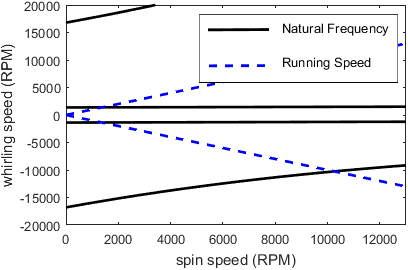
\includegraphics[scale=.75]{./figures/Images/Figure_4}
			\caption{Example Campbell diagram}
			\label{fig:Figure_4}
		\end{figure}
		To further understand the effect that stiffness anisotropy has on the system, Figure \ref{fig:Figure_5} and \ref{fig:Figure_6}  display a cascade of amplitude plots with changing stiffness anisotropy between the horizontal and vertical planes. Viewing the theoretical data in this way allows for comparison of the two natural frequencies to experimental values just as the Campbell Diagram does. In addition, the cascaded plots depict how the shape of the amplitude plots change with varying anisotropy. Figure \ref{fig:Figure_5}  uses the amplitude of positive and negative frequencies to display the effect of anisotropy. The interaction between the first and second natural frequencies can be seen as the two get closer to one another. Negative whirling is dominant only between the two natural frequencies. When the two natural frequencies coincide, there is a highly circular positive whirl orbit. Experimental amplitude plots are used in conjunction with Figure \ref{fig:Figure_5}  \& \ref{fig:Figure_6}  to choose the correct anisotropy at which the characteristic shape matches.\par 
		The skew angle, $\chi$, and the eccentricity, $\varepsilon$, are determined next by independent methods. Eccentricity can be determined by simulating the theoretical model under varying eccentricities until the magnitude of the vibration is equivalent to that of the experimental results. The value was determined to be $9\e{-4}  m$. The skew angle can be quantified using a similar technique. But the skew angle is closely related to the amplitude of vibration in the two orthogonal directions, $x$ and $y$, as well as the disk tilting angles, $\theta_x$ and $\theta_y$. In order to measure the tilting angles in the experiment, there were two sets of orthogonal transducers. One before the disk on the shaft and the other after the disk. This displacement between the two sets of transducers allows for an approximation of the angles of tilt. Assuming no bending of the shaft, the angle is deduced from a pivot about Bearing B, with the angle being equal to the inverse tangent of the ratio of difference in displacement between the transducers, and the distance between the transducers. Then the simulation is run with varying values of $\chi$ to match the amplitude of angles and displacements to the experiment. The value was determined to be 0.09 radians.\par 
		\begin{figure}[H]
			\centering
			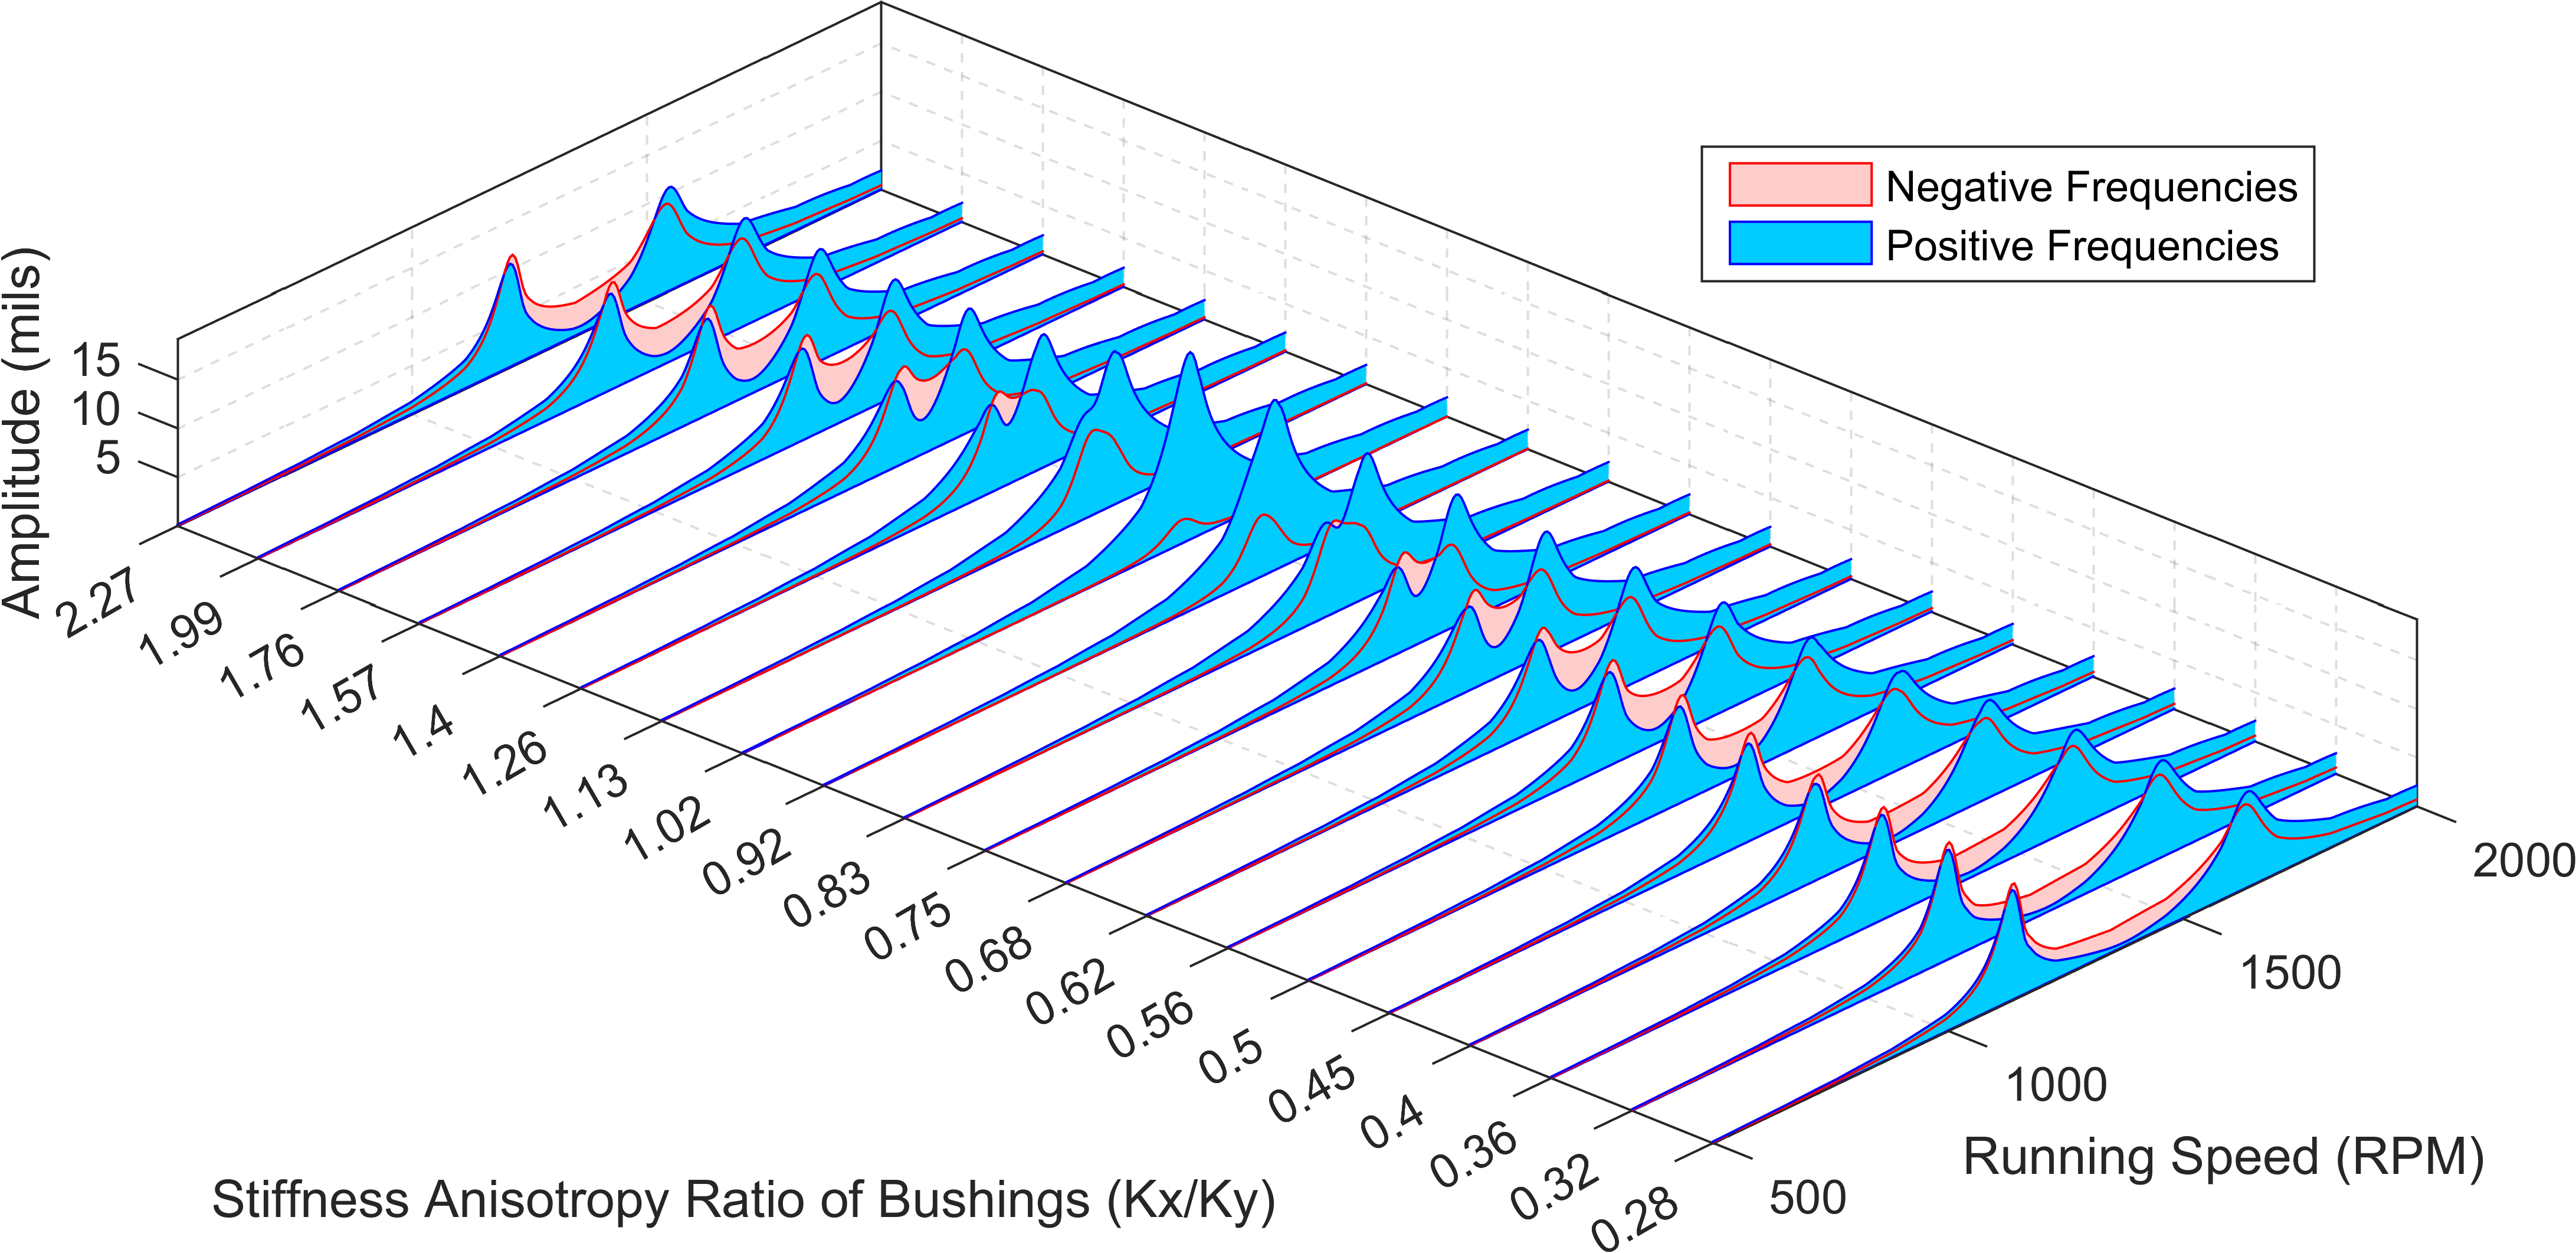
\includegraphics[width=.75\linewidth]{./figures/Images/Figure_5}
			\caption{3D cascading plot demonstrating the impact of stiffness anisotropy on positive/negative frequencies}
			\label{fig:Figure_5}
		\end{figure}
		\begin{figure}[H]
			\centering
			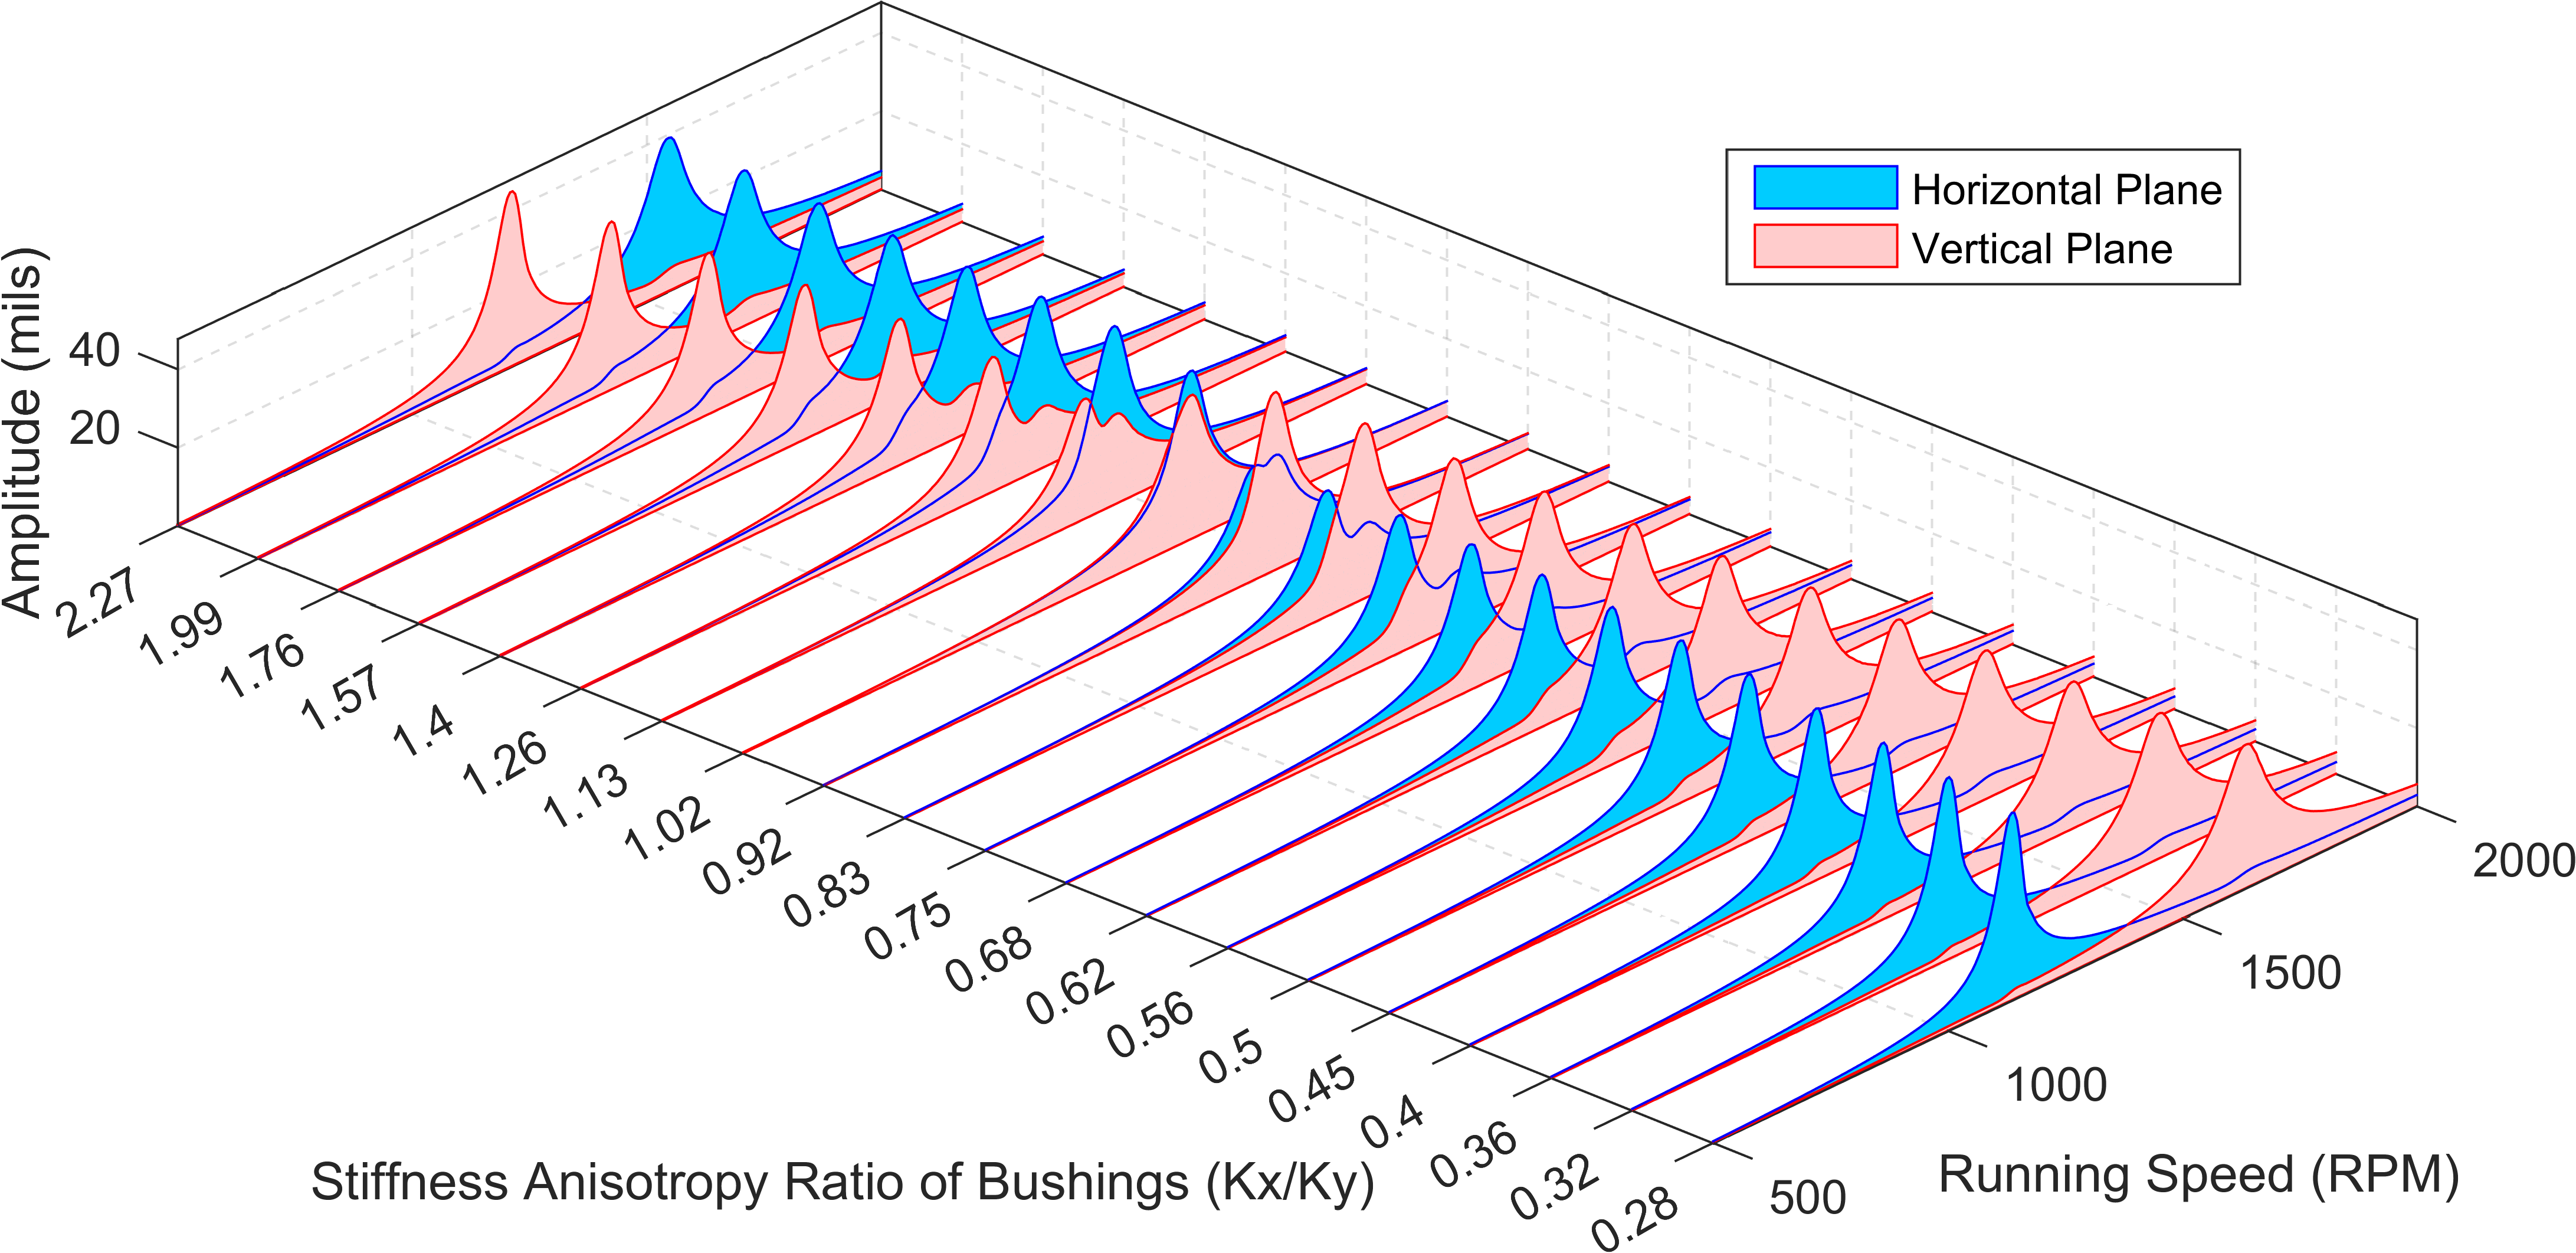
\includegraphics[width=.75\linewidth]{./figures/Images/Figure_6}
			\caption{3D cascading plot demonstrating the impact of stiffness anisotropy on horizontal/vertical frequencies}
			\label{fig:Figure_6}
		\end{figure}

	\section{Produce full spectrum plots from orthogonal transducers }
		The purpose of this work was to produce figures that represent vibration amplitude data from theoretical models in a way that is comparable to figures produced by the ADRE Sxp software. This allows the analysis of theoretical models with confidence in the representation of the data with figures such as the Bode plot, the Cascade plot, and full spectrum plots. The major achievement in producing the figures was obtaining phase lag angles between two signals. Another achievement was producing spectrum plots with both positive and negative frequencies (Full Spectrum plots).\par 
		Full spectrum plots are more complete in displaying the information contained in a Fourier Transform. In the frequency domain, negative frequencies pertain to vibration of the rotor that is precessing in the opposite rotational direction than that of the rotor rotational direction. The full spectrum plot is produced by first coupling the orthogonal transducer signals into a complex signal and then performing a Fourier transform. The transform on the complex data results in frequency information both negative and positive.\par 
		Negative frequencies tell a lot about the system, especially when they are greater than their positive counterpart. When the negative frequency vibration is greater in amplitude, the precession is said to be in the “reverse” direction. This can be vital information in diagnosing a problem in a real rotor system. In the case explored here it can be a sign of both, strong gyroscopic moments, as well as anisotropy of the stiffness from the shaft or the bearings. Another example is the rub in a fluid film bearing which manifests itself as a negative precession at twice the running speed of the rotor. This problem would be more difficult to diagnose without the knowledge of negative frequencies.\par 
		In order to verify that the MATLAB code of our method would produce accurate frequency data, the Fast Fourier Transform, or FFT, of a steady state signal was compared to the FFT produced by the ADRE 408 with ADRE Sxp software. Both the amplitude and frequency of positive and negative frequency components was verified by comparison as demonstrated by the comparison of Figure \ref{fig:Figure_7}  and \ref{fig:Figure_8} .\par 
		\begin{figure}[H]
			\centering
			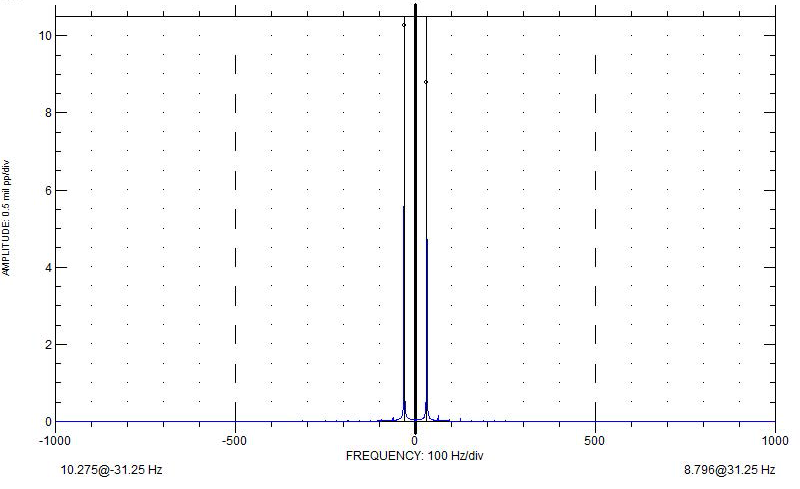
\includegraphics[width=.6\linewidth]{./figures/Images/Figure_7}
			\caption{Full Spectrum plot produced with the ADRE sxp software}
			\label{fig:Figure_7}
		\end{figure}
		\begin{figure}[H]	
			\centering
			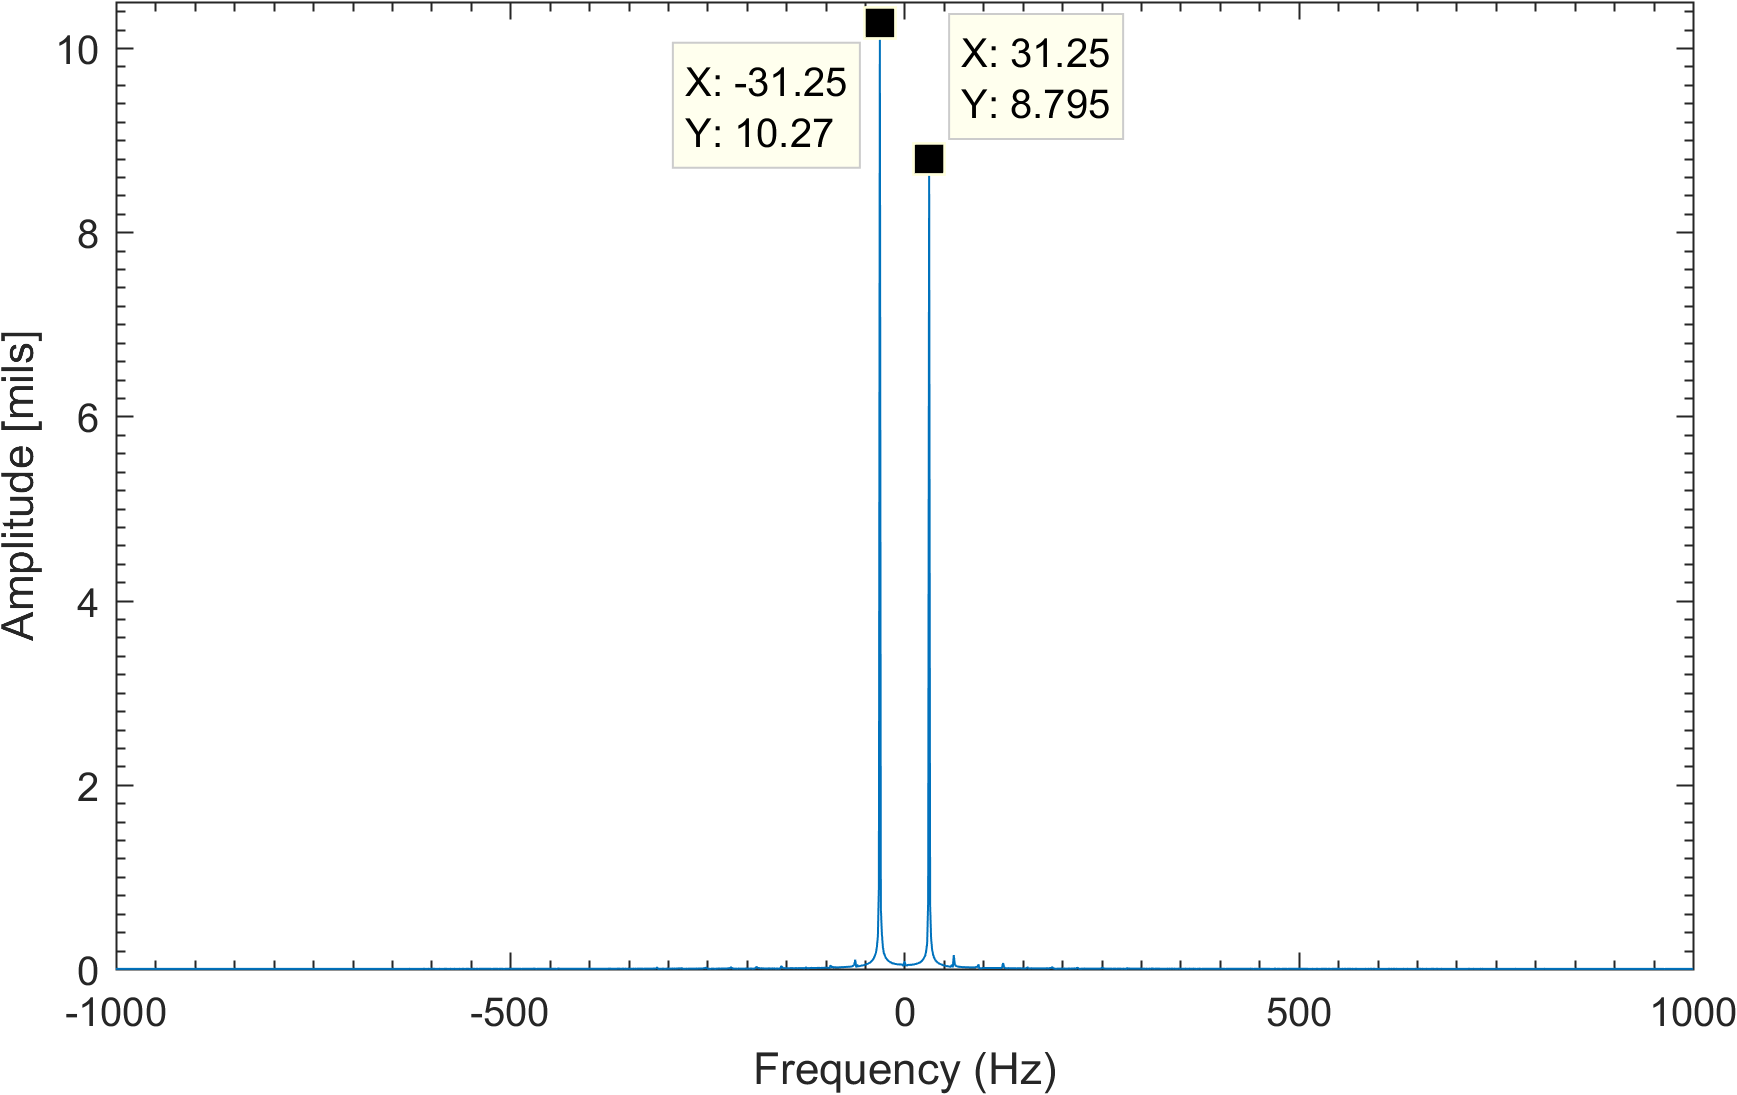
\includegraphics[width=.6\linewidth]{./figures/Images/Figure_8}
			\caption{Full Spectrum plot produced with using our method}
			\label{fig:Figure_8}
		\end{figure}
	\section{Produce Bode plots from orthogonal transducers }
		The process for producing phase lag angles begins with segmenting the data into windows of a fixed number of samples. This is because most rotordynamic data comes in the form of a “start-up” or a “run-down”. In both of these scenarios, the rotational speed of the rotor is continuously changing, as demonstrated by Figure \ref{fig:Figure_9a}. This change deters capturing both time and frequency information. Segmenting the data provides small windows on which analysis can be performed as if the signal was a constant frequency within the window, as demonstrated in Figure \ref{fig:Figure_9b}. For a segment of data in which the frequency is not changing, a Fourier Transform can be applied to obtain the frequency spectrum of the signal. In this frequency domain provided by the Fourier Transform, the phase angle of each frequency can be obtained as well as the amplitude of vibration of each frequency. In order to calculate the phase lag from one signal to another, this phase angle is compared for the same frequency of each signal in the same window in time. This process is done for each window through the entire length of data producing a phase angle for each window.\par 
		The Bode plot is ubiquitous in rotating machinery diagnostics and can be used to characterize a system fairly thoroughly. Phase angle is a vital part of the bode plot and can shed light on many phenomenon One of the main goals in this paper is to demonstrate the ability to produce accurate phase lag information from two signals. As seen in the Bode plot of Figure \ref{fig:Figure_10} , the MATLAB code based on complex FFT strategy produces phase lag information nearly identical to the phase lag information produced with the ADRE system using the same transducer data.\par 
		\begin{figure}[H]
			\begin{subfigure}[b]{.5\linewidth}	
				\centering
				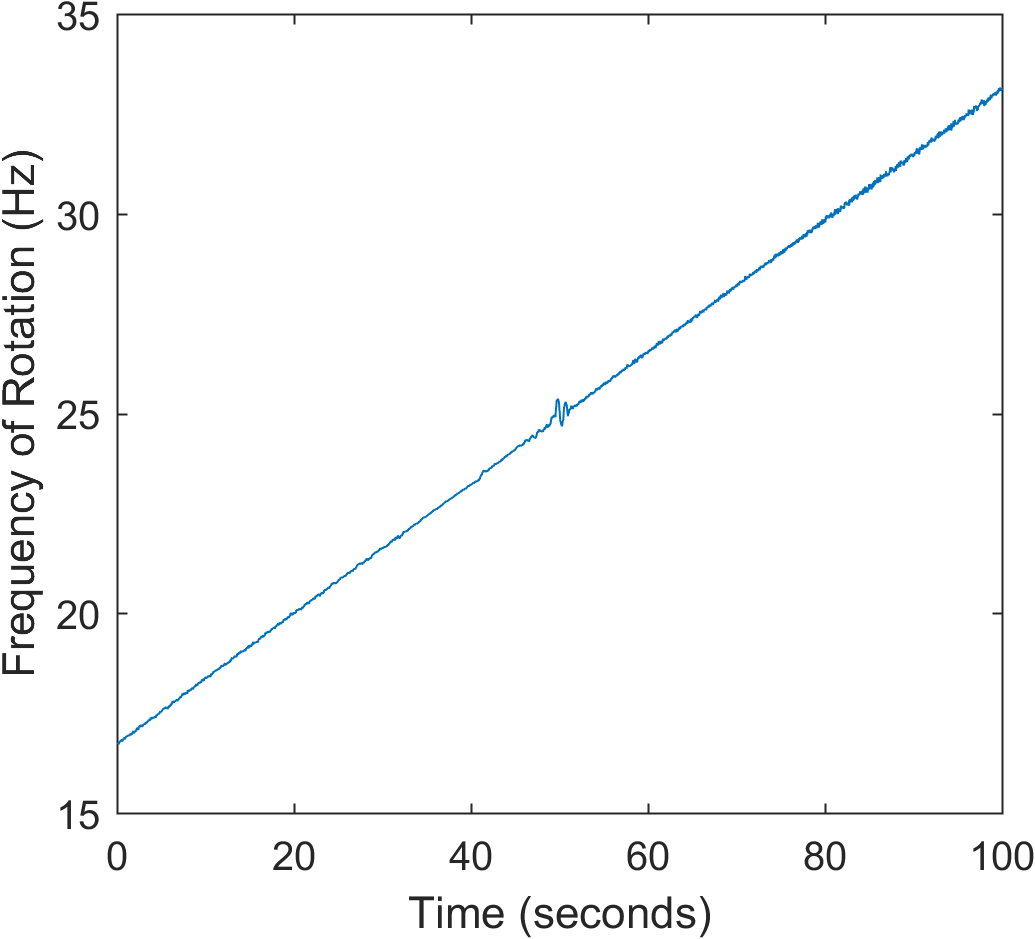
\includegraphics[width=1\textwidth]{./figures/Images/Figure_9a}
				\caption{Rotational speed change over time}
				\label{fig:Figure_9a}
			\end{subfigure}
			\begin{subfigure}[b]{.5\linewidth}
				\centering
				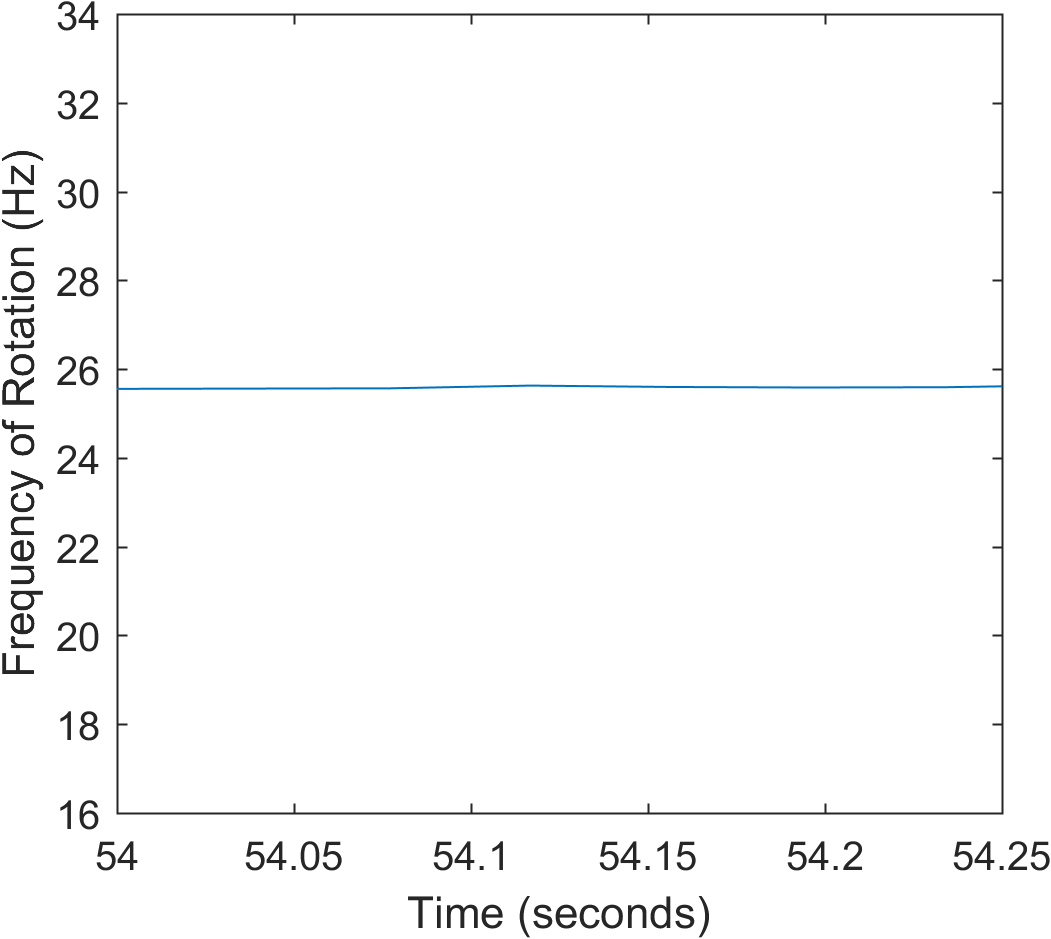
\includegraphics[width=1\textwidth]{./figures/Images/Figure_9b}
				\caption{Rotational speed change over a window in time}
				\label{fig:Figure_9b}
			\end{subfigure}
			\caption{Steady-state approximation demonstration}
			\label{fig:Figure_9}
		\end{figure}
		This ability to produce phase lag information from any transducer data allows accurate comparison of theoretical and experimental data. The MATLAB code that produces these plots also allows the ability of tuning the resolution of the phase and amplitude information, gaining accuracy in either time or frequency. The phase lag calculation accuracy is determined by the number of cycles analyzed in each window, so the larger the window, the better the phase information. But, as the window gets larger, the accuracy of speed is diminished.\par 
		\begin{figure}[H]	
			\centering
			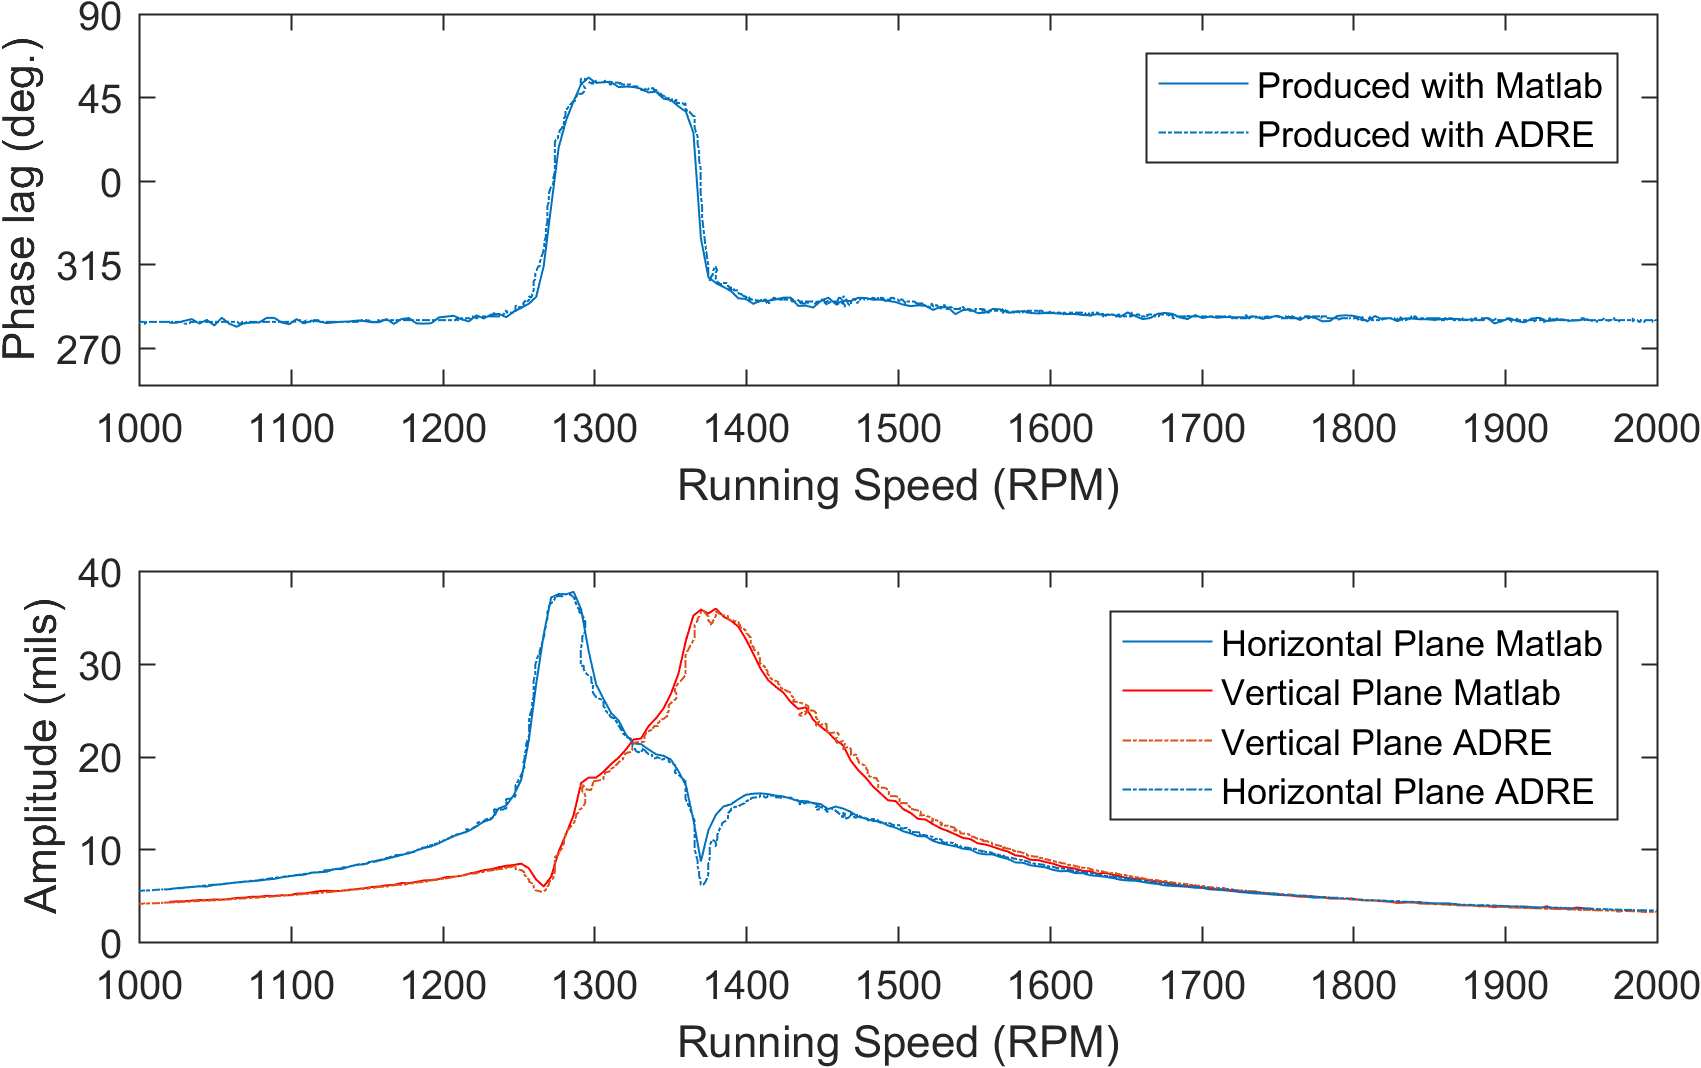
\includegraphics[width=.75\linewidth]{./figures/Images/Figure_10}
			\caption{Bode plot for verification of the phase angle technique}
			\label{fig:Figure_10}
		\end{figure}
	\section{Theoretical and experimental comparison}
		The comparison of experiment and theoretical model developed in this research were performed. The geometric and other parameters of the rotor kit are shown in table 1.\par 
		\begin{figure}[H]	
			\centering
			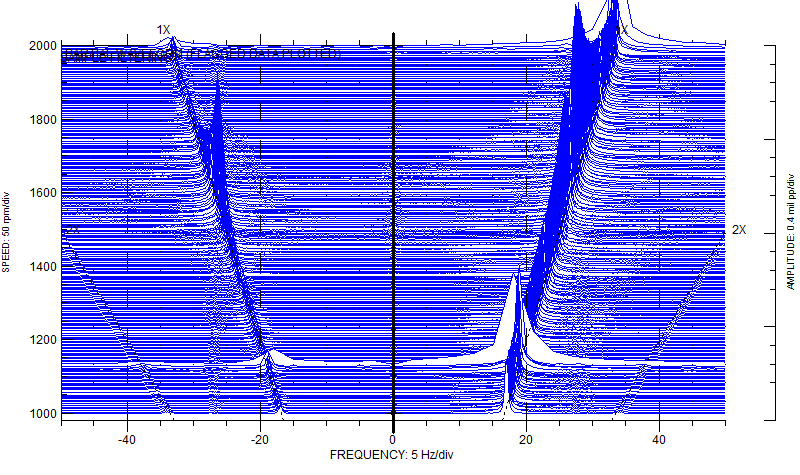
\includegraphics[width=.75\linewidth]{./figures/Images/Figure_11}
			\caption{Experimental Cascade plot directly produced by the ADRE sxp software}
			\label{fig:Figure_11}
		\end{figure}
		\begin{figure}[H]	
			\centering
			\includegraphics[width=.75\linewidth]{./figures/Images/Figure_12}
			\caption{Re-constructed 3D experimental full-spectrum cascade plot using our strategy}
			\label{fig:Figure_12}
		\end{figure}
		\begin{figure}[H]	
			\centering
			\includegraphics[width=.75\linewidth]{./figures/Images/Figure_13}
			\caption{3D theoretical full-spectrum cascade plot using our strategy}
			\label{fig:Figure_13}
		\end{figure}
		The full-spectrum cascade plot is a vital tool for analysis in rotating machinery. The cascade plot depicts how the vibrations change with time. With the addition of the full spectrum in these cascade plots, the negative frequencies provide insight for diagnostics of certain rotor issues, such as misalignment of disk axis with the rotor axis. Just as with the FFT and Bode plots, the cascade plot produced with our MATLAB code using complex FFT strategy is compared with the cascade produced with the ADRE software to validate the method. From figure \ref{fig:Figure_11}, \ref{fig:Figure_12} and \ref{fig:Figure_13}, we can see the results are similar and good enough to validate our full-spectrum strategy through experiment. Furthermore, MATLAB has the ability to display data in three dimensions as shown in the figures (\cite{Southwick},\cite{Southwick 94},\cite{Dimarogonas}). With proper tuning of window size and sampling frequency, the cascade plot can display a host of rotordynamic phenomenon.\par 
		\begin{figure}[H]	
			\centering
			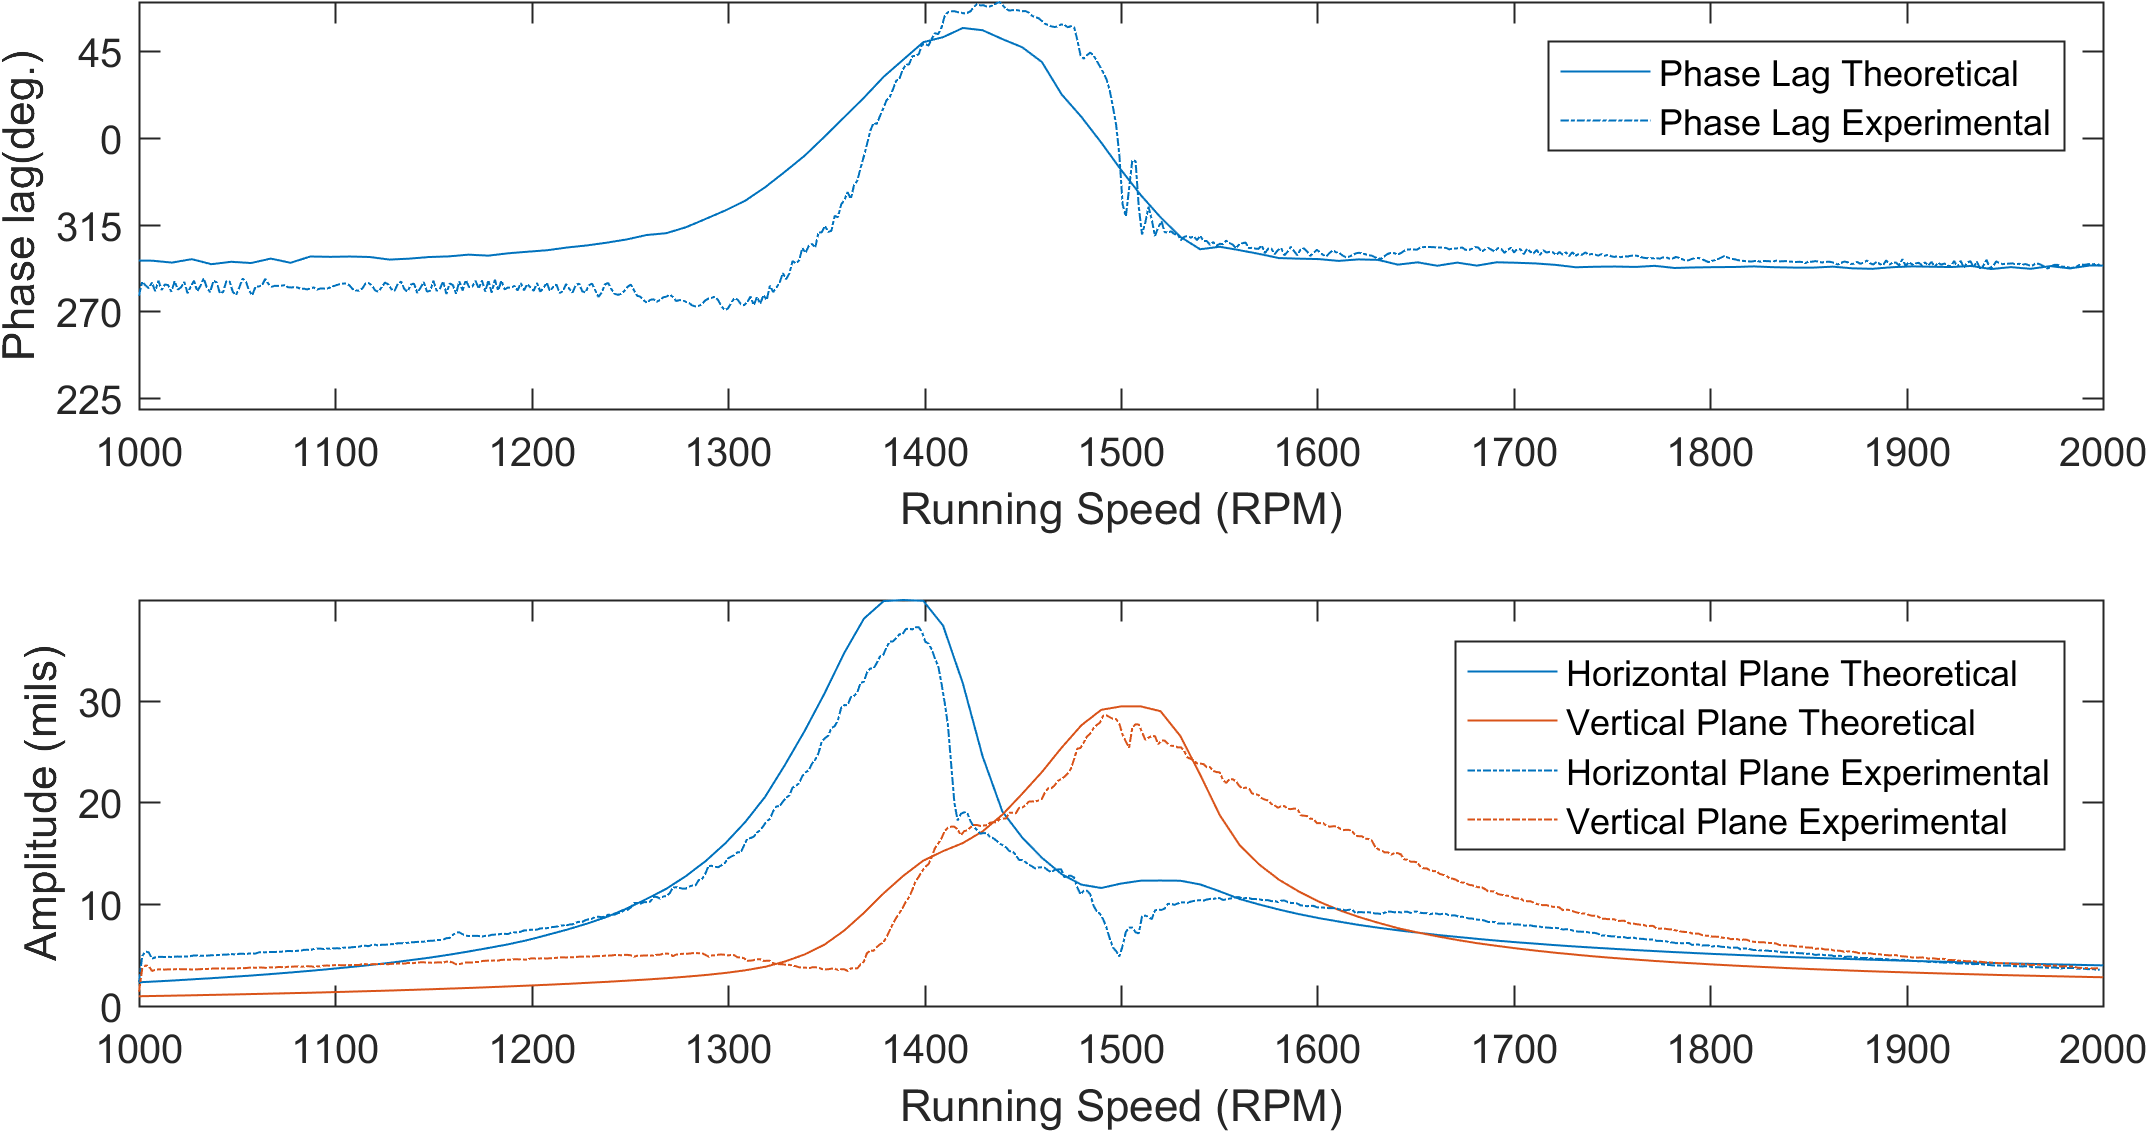
\includegraphics[width=1\linewidth]{./figures/Images/Figure_14}
			\caption{Bode plot, Experimental vs. Theoretical}
			\label{fig:Figure_14}
		\end{figure}
		The Bode plot of Figure \ref{fig:Figure_14} compares the startup amplitude and phase angle of the theoretical model and the experiment. Because both the experimental and the theoretical results were processed using our strategy with the same MATLAB code to produce these plots, comparisons can be confidently drawn. The phase angles are of a phase lag from the X transducer and from the Y transducer. The two transducers are 270 positive degrees apart around the shaft.\par 
		\begin{figure}[H]	
			\centering
			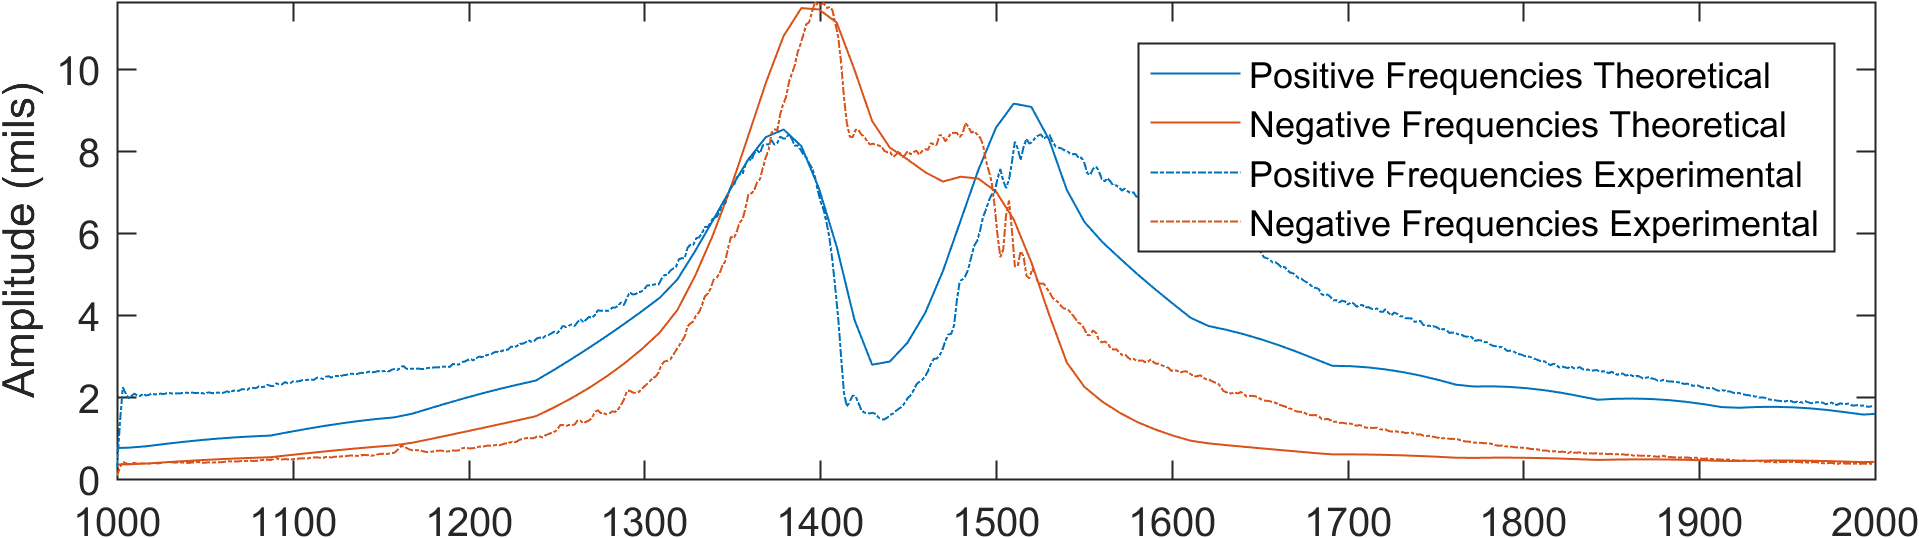
\includegraphics[width=1\linewidth]{./figures/Images/Figure_15}
			\caption{Positive/Negative frequency comparison, Experimental vs. Theoretical}
			\label{fig:Figure_15}
		\end{figure}
		Observing the comparison of positive and negative frequencies as done in Figure \ref{fig:Figure_15} allows the detection of backward or forward whirl. When the negative frequency amplitude is greater than that of the positive frequency, the whirl is “backward”. Backward whirl describes the phenomenon of precession of the shaft vibration rotating opposite to the rotation of the shaft. Comparison to the typical horizontal vs. vertical amplitude plot shows that the crossover from positive to negative whirl occurs when either the horizontal or vertical vibration amplitudes drop.\par 
		\begin{figure}[H]
			\begin{subfigure}[b]{.5\linewidth}	
				\centering
				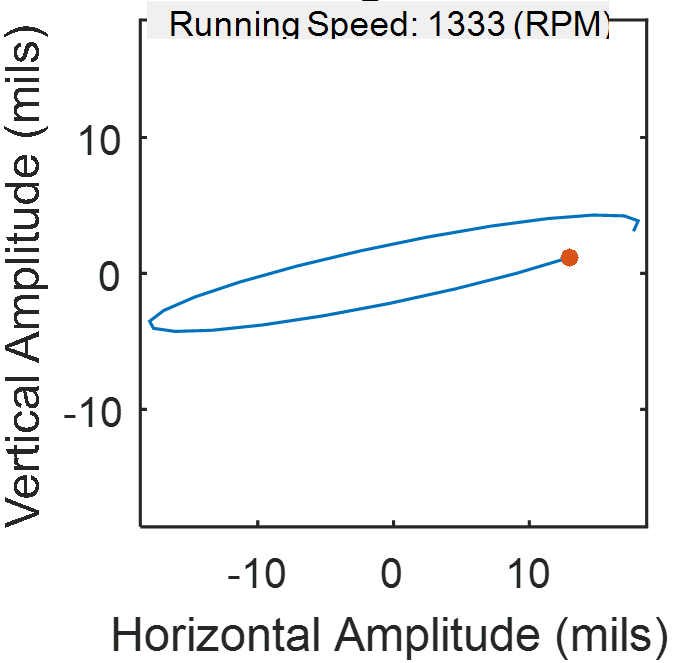
\includegraphics[width=.75\textwidth]{./figures/Images/Figure_16a}
				\caption{Experimental 1333 RPM orbit}
				\label{fig:Figure_16a}
			\end{subfigure}
			\begin{subfigure}[b]{.5\linewidth}
				\centering
				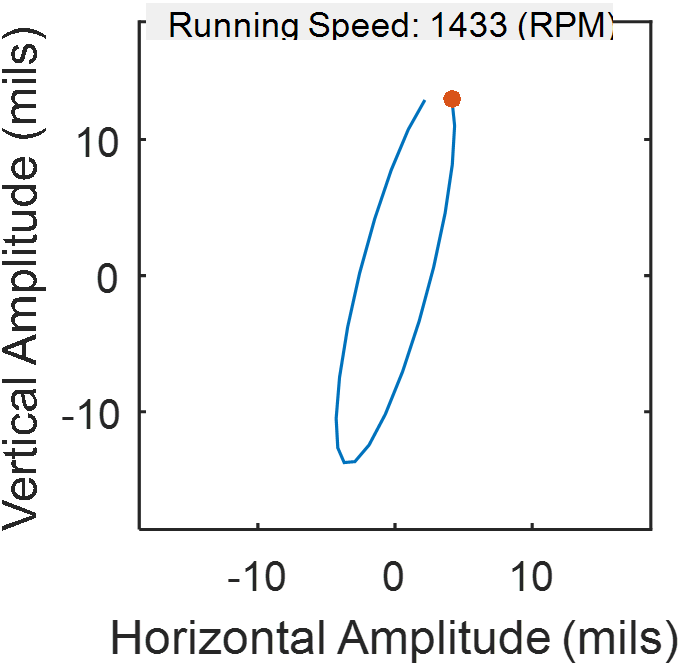
\includegraphics[width=.75\textwidth]{./figures/Images/Figure_16b}
				\caption{Experimental 1433 RPM orbit}
				\label{fig:Figure_16b}
			\end{subfigure}
			\begin{subfigure}[b]{.5\linewidth}
				\centering
				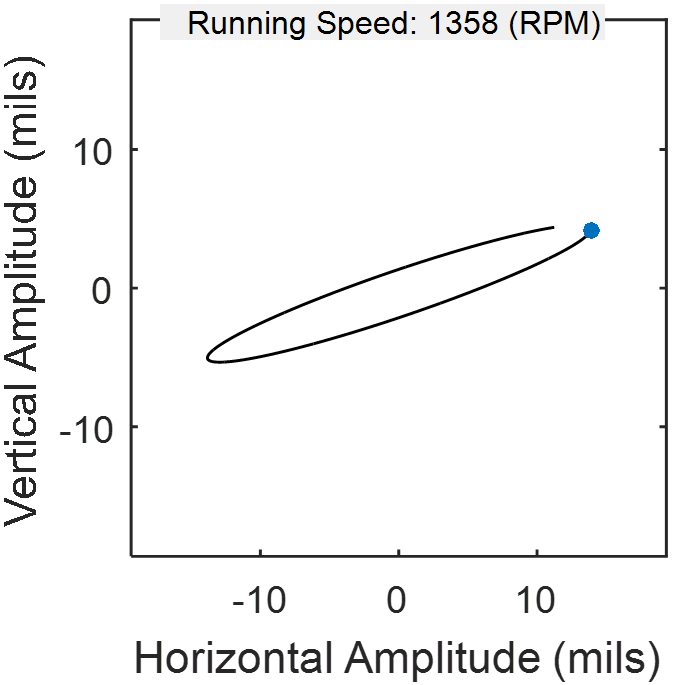
\includegraphics[width=.75\textwidth]{./figures/Images/Figure_16c}
				\caption{Theoretical 1358 RPM orbit}
				\label{fig:Figure_16c}
			\end{subfigure}
			\begin{subfigure}[b]{.5\linewidth}
				\centering
				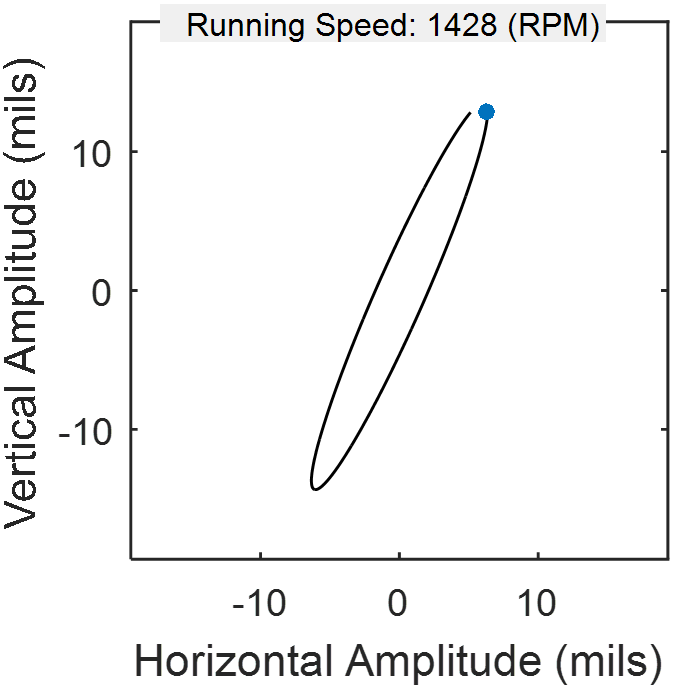
\includegraphics[width=.75\textwidth]{./figures/Images/Figure_16d}
				\caption{Theoretical 1428 RPM orbit}
				\label{fig:Figure_16d}
			\end{subfigure}
			\caption{Orbit plots fo filtered experimental data compared to theoretical predictions at similar speeds}
			\label{fig:Figure_16}
		\end{figure}
		Orbit plots of Figure \ref{fig:Figure_16} are created using experimental and theoretical data. The orbits of experimental data contain the key-phasor dot to mark the beginning of a rotation from a fixed location on the shaft. This allows the determination of the orbit rotation direction. For all of the orbit plots, the shaft was rotating in the counter-clockwise direction. Therefore, an orbit in the clockwise direction is in the “reverse” direction. Experimental data was filtered using a tracking filter for the orbit plots. Since a once per turn reference is unavailable for theoretical data, the orbits are plotted with a reference dot at the maximum $x$ value for that orbit.\par 
		\begin{figure}[H]	
			\centering
			\includegraphics[width=1\linewidth]{./figures/Images/Figure_17}
			\caption{Experimental 3D Orbit plot produced by our strategy}
			\label{fig:Figure_17}
		\end{figure}
		\begin{figure}[H]	
			\centering
			\includegraphics[width=1\linewidth]{./figures/Images/Figure_18}
			\caption{Theoretical 3D Orbit plot}
			\label{fig:Figure_18}
		\end{figure}
		Orbit plots are cascaded in increasing rotational speed in the 3D orbit plots of Figures \ref{fig:Figure_17} and \ref{fig:Figure_18}. This cascade of orbits gives a sense of how the natural frequencies are physically manifested in these startups. This 3D orbit plot lends a more intuitive representation of the data and at the same time, important characteristics such as phase lag, amplitudes and reverse precession can be discerned from the plot. This plot was also useful in comparing the theoretical model to the experimental data, because it demonstrates magnitude as well as general shape of the response of the entire orbit in one plot. Also Figure \ref{fig:Figure_17} and \ref{fig:Figure_18} makes clear the effect of gyroscopic moments, as the shape of the elliptical orbits during peak amplitude vibrations are bent. The ADRE Sxp software does not produce this plot.\par 
	\section{Discussion and conclusions}
		3D cascade plots (Figures \ref{fig:Figure_12}, \ref{fig:Figure_13}) produced using our complex FFT strategy clearly display the full vibration spectrum and complement those produced with the ADRE Sxp software (Figure \ref{fig:Figure_11}). Both the theoretical model and the experimental results display a sudden dip in amplitude of positive frequencies between the two natural frequencies (Figures \ref{fig:Figure_12},\ref{fig:Figure_13}). This dip is coupled with an increase in negative frequencies, resulting in reverse orbits for a period in time. These negative orbits can be seen in Figure \ref{fig:Figure_16}. The theoretical model suggested a strong influence from the relative phase angle of the skew to the eccentricity. Some values of phase difference offered completely positive orbits through the natural frequency, while others offered highly negative orbits. This is the greatest contribution from the skew angle, as without the consideration of it, the amount of negative to positive vibration could not be easily altered in the theoretical model.\par 
		In this paper, the dynamic behavior of a flexible shaft with an overhung disk has been studied by employing full spectrum analysis. Anisotropic bearing stiffness and the effect of gyroscopic moments are considered in our classic theoretical model. Some of the parameters which are difficult to directly measure are estimated by combination of theoretical calculation and experimental results. Full spectrum analysis is applied to the system to reveal some interesting backward whirl vibration phenomena due to the interaction of anisotropy of the stiffness of the bearings, flexibility of the shaft and gyroscopic effect. Phenomena such as these cannot be disclosed by traditional half spectrum FFT. 3D cascade full spectrum plots from theoretical model are compared to those from experiments. Our full spectrum cascade plots using complex FFT strategy capture more detail in the vibration response of the system than the typical cascade plots. Filtered orbit plots with the key-phasor dots at different speed demonstrate forward and backward whirls. Methods for identifying the eccentricity and skew angle of the disk are presented. Also, the effect of the skew angle is determined by comparison of experiment and theory. The skew angle is determined by comparing theoretical angular amplitudes to experimental angular amplitudes. Bearing stiffness is determined through a method of matching theoretical and experimental natural frequencies. Consideration of the gyroscopic moments introduces speed as another dependent variable in the equation for natural frequency, making the process of matching an iterative one.\par 
	\section{Acknowledgments}
		The authors acknowledge the Donald E. Bently Center for Engineering Innovation at California Polytechnic State University San Luis Obispo for support of this work.\par 

\nocite{*}
\bibliography{bibliography}

% Indents Appendix in Table of Contents
\makeatletter
\addtocontents{toc}{\let\protect\l@chapter\protect\l@section}
\makeatother

% Hack to make Appendices to appear in Table of Contents
\addtocontents{toc}{%
   \noindent APPENDICES
}
\begin{appendices}
%\chapter{Bernoulli-Euler Beam equation}\label{Bernoulli-Euler Beam equation}


Assumptions used to derive the Bernoulli-Euler beam equation are (Complete derivation in \cite{craig2006fundamentals}):
\begin{enumerate}
	\item Beam is bending in a plane, in this case in the y-direction, where the x-direction is along the length of the beam.
	\item The  neutral axis undergoes no deformation in the longitudinal direction.
	\item Cross sections remain plane and perpendicular to the nuetral axis.
	\item The material is linear-elastic.
	\item Stresses in the y and z direction are negligible compared to those in the x direction.
	\item Rotary inertial effects are not considered.
	\item Mass density is constant at each cross section, so that each mass center is coincident with the centroid of that section.
\end{enumerate}
Using kinematics and assumptions 2 \& 3, the strain in the x direction may be related to the curvature of the beam, $\mu(x,t)$, and the distance from the neutral axis by
\begin{equation} \label{eq:curvature}
\epsilon=-\dfrac{y}{\mu}
\end{equation}
then, with assumption 4 \& 7 the relation from curvature to moment is
\begin{equation} \label{eq:curv_moment}
M(x,t)=\dfrac{EI}{\mu}
\end{equation}
\begin{figure}
	\centering
	\def\svgwidth{300pt}
	\import{figures/}{BeamFBD.pdf_tex}
	\caption{Free body diagram of a beam section in planar bending.}
	\label{fig:BeamFBD}
\end{figure}
where $ E $, Young's modulus, and $ I $, area moment of inertia are constant in cross sections. By using Newton's laws and the free body diagram of a single beam element, see Figure \ref{fig:BeamFBD}, the equations of motion are summarized as:
\begin{equation} \label{eq:Newton}
\sum{F_y}=\Delta m \ddot{v} \quad \textrm{\&} \quad \sum{M_G}=0
\end{equation}
Moment equation is represented as moments summarized at the center of mass, $ G $. The right hand side of moment equation of EOM \eqref{eq:Newton} is know to be null due to assumption 6. Applying Newton's equations \eqref{eq:Newton} to the FBD of Figure \ref{fig:BeamFBD} results in the force equation
\begin{equation} \label{eq:force_EOM}
F(x,t)-F(x+\Delta x,t)=\rho A\Delta x \frac{\partial^2 v}{\partial t^2}
\end{equation}
and moment equation
\begin{equation} \label{eq:moment_EOM}
-M(x,t) + M(x+\Delta x,t) + F(x,t)\left( \frac{-\Delta x}{2}\right)  + \left[-F(x+\Delta x,t)\right] \left(\frac{\Delta x}{2}\right) = 0
\end{equation}
Taking the limit of equations \eqref{eq:force_EOM} \& \eqref{eq:moment_EOM} as $ \Delta x \rightarrow 0 $ results in equations \eqref{eq:force_EOM_partial} \& \eqref{eq:moment_EOM_partial} respectively.
\begin{equation} \label{eq:force_EOM_partial}
\frac{\partial F}{\partial x}=-\rho A \frac{\partial^2 v}{\partial t^2}
\end{equation} 
\begin{equation} \label{eq:moment_EOM_partial}
\frac{\partial M}{\partial x} - F=0
\end{equation}
Assuming the beam slope, $ \frac{\partial v}{\partial x} $, remains relatively small, then linearized curvature of the beam is inversely related to $ \frac{\partial^2 v}{\partial x^2} $. Substituting this linearized curvature in \eqref{eq:curv_moment} produces
\begin{equation} \label{eq:moment_curvature_partial}
M(x,t)=EI\frac{\partial^2 v}{\partial x^2}
\end{equation}
Using linearized moment equation \eqref{eq:moment_curvature_partial}, combined with \eqref{eq:force_EOM_partial} \&  \eqref{eq:moment_EOM_partial} lends the Euler beam equation
\begin{equation} \label{eq:euler_beam_equation}
\frac{\partial^2}{\partial x^2} \left(EI\frac{\partial^2 v}{\partial x^2}\right) = -\rho A\frac{\partial^2 v}{\partial t^2}
\end{equation}
This is the governing differential equation for transverse motion of a slender beam. This equation is not suitable for an application involving lengths that are not much greater than the width of the beam \cite{genta2007dynamics}.
%\chapter{RotorFEM MATLAB Code for Constructing and Analyzing FEM Models}
%\section{Main Object File}
%\lstinputlisting[language=Matlab]{appendices/code/RotorFEM.m}
%\section{Matrix Assembly File}
%\lstinputlisting[language=Matlab]{appendices/code/Assem.m}
%\section{Elemental Matrices}
%\lstinputlisting[language=Matlab]{appendices/code/TBeam.m}
%\lstinputlisting[language=Matlab]{appendices/code/Disk.m}
%\lstinputlisting[language=Matlab]{appendices/code/Bear.m}
%\section{Plotting Functions}
%\lstinputlisting[language=Matlab]{appendices/code/RootLocus.m}
%\lstinputlisting[language=Matlab]{appendices/code/Campbell.m}
%\lstinputlisting[language=Matlab]{appendices/code/Stability.m}
%\lstinputlisting[language=Matlab]{appendices/code/Damping.m}
%\lstinputlisting[language=Matlab]{appendices/code/Shape.m}
%\lstinputlisting[language=Matlab]{appendices/code/FreqResponse.m}
%\chapter{RotorDAQ MATLAB Code for Analyzing Vibration Signals}
%\section{Main Object File}
%\lstinputlisting[language=Matlab]{appendices/code/RotorDAQ/RotorData.m}
%\section{Plotting Functions}
%\lstinputlisting[language=Matlab]{appendices/code/RotorDAQ/bode.m}
%\lstinputlisting[language=Matlab]{appendices/code/RotorDAQ/cascade.m}
%\lstinputlisting[language=Matlab]{appendices/code/RotorDAQ/orbit3.m}
%\lstinputlisting[language=Matlab]{appendices/code/RotorDAQ/orbitAnimation.m}
\end{appendices}

\end{document}
